\documentclass[twoside]{book}

% Packages required by doxygen
\usepackage{calc}
\usepackage{doxygen}
\usepackage{graphicx}
\usepackage[utf8]{inputenc}
\usepackage{makeidx}
\usepackage{multicol}
\usepackage{multirow}
\usepackage{textcomp}
\usepackage[table]{xcolor}

% Font selection
\usepackage[T1]{fontenc}
\usepackage{mathptmx}
\usepackage[scaled=.90]{helvet}
\usepackage{courier}
\usepackage{amssymb}
\usepackage{sectsty}
\renewcommand{\familydefault}{\sfdefault}
\allsectionsfont{%
  \fontseries{bc}\selectfont%
  \color{darkgray}%
}
\renewcommand{\DoxyLabelFont}{%
  \fontseries{bc}\selectfont%
  \color{darkgray}%
}

% Page & text layout
\usepackage{geometry}
\geometry{%
  a4paper,%
  top=2.5cm,%
  bottom=2.5cm,%
  left=2.5cm,%
  right=2.5cm%
}
\tolerance=750
\hfuzz=15pt
\hbadness=750
\setlength{\emergencystretch}{15pt}
\setlength{\parindent}{0cm}
\setlength{\parskip}{0.2cm}
\makeatletter
\renewcommand{\paragraph}{%
  \@startsection{paragraph}{4}{0ex}{-1.0ex}{1.0ex}{%
    \normalfont\normalsize\bfseries\SS@parafont%
  }%
}
\renewcommand{\subparagraph}{%
  \@startsection{subparagraph}{5}{0ex}{-1.0ex}{1.0ex}{%
    \normalfont\normalsize\bfseries\SS@subparafont%
  }%
}
\makeatother

% Headers & footers
\usepackage{fancyhdr}
\pagestyle{fancyplain}
\fancyhead[LE]{\fancyplain{}{\bfseries\thepage}}
\fancyhead[CE]{\fancyplain{}{}}
\fancyhead[RE]{\fancyplain{}{\bfseries\leftmark}}
\fancyhead[LO]{\fancyplain{}{\bfseries\rightmark}}
\fancyhead[CO]{\fancyplain{}{}}
\fancyhead[RO]{\fancyplain{}{\bfseries\thepage}}
\fancyfoot[LE]{\fancyplain{}{}}
\fancyfoot[CE]{\fancyplain{}{}}
\fancyfoot[RE]{\fancyplain{}{\bfseries\scriptsize Generated on Thu Apr 17 2014 17\-:33\-:32 for Hand\-Detection by Doxygen }}
\fancyfoot[LO]{\fancyplain{}{\bfseries\scriptsize Generated on Thu Apr 17 2014 17\-:33\-:32 for Hand\-Detection by Doxygen }}
\fancyfoot[CO]{\fancyplain{}{}}
\fancyfoot[RO]{\fancyplain{}{}}
\renewcommand{\footrulewidth}{0.4pt}
\renewcommand{\chaptermark}[1]{%
  \markboth{#1}{}%
}
\renewcommand{\sectionmark}[1]{%
  \markright{\thesection\ #1}%
}

% Indices & bibliography
\usepackage{natbib}
\usepackage[titles]{tocloft}
\setcounter{tocdepth}{3}
\setcounter{secnumdepth}{5}
\makeindex

% Hyperlinks (required, but should be loaded last)
\usepackage{ifpdf}
\ifpdf
  \usepackage[pdftex,pagebackref=true]{hyperref}
\else
  \usepackage[ps2pdf,pagebackref=true]{hyperref}
\fi
\hypersetup{%
  colorlinks=true,%
  linkcolor=blue,%
  citecolor=blue,%
  unicode%
}

% Custom commands
\newcommand{\clearemptydoublepage}{%
  \newpage{\pagestyle{empty}\cleardoublepage}%
}


%===== C O N T E N T S =====

\begin{document}

% Titlepage & ToC
\hypersetup{pageanchor=false}
\pagenumbering{roman}
\begin{titlepage}
\vspace*{7cm}
\begin{center}%
{\Large Hand\-Detection \\[1ex]\large 1 }\\
\vspace*{1cm}
{\large Generated by Doxygen 1.8.5}\\
\vspace*{0.5cm}
{\small Thu Apr 17 2014 17:33:32}\\
\end{center}
\end{titlepage}
\clearemptydoublepage
\tableofcontents
\clearemptydoublepage
\pagenumbering{arabic}
\hypersetup{pageanchor=true}

%--- Begin generated contents ---
\chapter{Main Page}
\label{index}\hypertarget{index}{}\begin{TabularC}{2}
\hline
\rowcolor{lightgray}{\bf Library }&Simple\-Opt \\\cline{1-2}
\rowcolor{lightgray}{\bf Author }&Brodie Thiesfield \mbox{[}code at jellycan dot com\mbox{]} \\\cline{1-2}
\rowcolor{lightgray}{\bf Source }&\href{http://code.jellycan.com/simpleopt/}{\tt http\-://code.\-jellycan.\-com/simpleopt/} \\\cline{1-2}
\end{TabularC}
\hypertarget{index_SimpleOpt}{}\section{Simple\-Opt}\label{index_SimpleOpt}
A cross-\/platform library providing a simple method to parse almost any of the standard command-\/line formats in use today.

See the \hyperlink{_simple_opt_8h}{Simple\-Opt } documentation for full details.\hypertarget{index_SimpleGlob}{}\section{Simple\-Glob}\label{index_SimpleGlob}
A cross-\/platform file globbing library providing the ability to expand wildcards in command-\/line arguments to a list of all matching files.

See the \hyperlink{}{Simple\-Glob } documentation for full details. 
\chapter{Hand\-Detection}
\label{md___users_raphaeldendooven__documents_school_2013-2014__thesis__master__programs__hand_detection__r_e_a_d_m_e}
\hypertarget{md___users_raphaeldendooven__documents_school_2013-2014__thesis__master__programs__hand_detection__r_e_a_d_m_e}{}
Algoritm to detect hands in a moving picture file 
\chapter{Hierarchical Index}
\section{Class Hierarchy}
This inheritance list is sorted roughly, but not completely, alphabetically\-:\begin{DoxyCompactList}
\item \contentsline{section}{F\-F\-L\-D\-:\-:detail\-:\-:Area\-Comparator}{\pageref{class_f_f_l_d_1_1detail_1_1_area_comparator}}{}
\item \contentsline{section}{F\-F\-L\-D\-:\-:detail\-:\-:Bilinear}{\pageref{struct_f_f_l_d_1_1detail_1_1_bilinear}}{}
\item \contentsline{section}{Center\-Point}{\pageref{struct_center_point}}{}
\item \contentsline{section}{Cluster}{\pageref{class_cluster}}{}
\item \contentsline{section}{C\-Simple\-Opt\-Templ$<$ S\-O\-C\-H\-A\-R $>$}{\pageref{class_c_simple_opt_templ}}{}
\item \contentsline{section}{Det\-Body}{\pageref{class_det_body}}{}
\item \contentsline{section}{Det\-Hand}{\pageref{class_det_hand}}{}
\item \contentsline{section}{Face\-Detection}{\pageref{class_face_detection}}{}
\item Generic\-Num\-Traits\begin{DoxyCompactList}
\item \contentsline{section}{Eigen\-:\-:Num\-Traits$<$ Array$<$ F\-F\-L\-D\-:\-:H\-O\-G\-Pyramid\-:\-:Scalar, F\-F\-L\-D\-:\-:H\-O\-G\-Pyramid\-:\-:Nb\-Features, 1 $>$ $>$}{\pageref{struct_eigen_1_1_num_traits_3_01_array_3_01_f_f_l_d_1_1_h_o_g_pyramid_1_1_scalar_00_01_f_f_l_d_179908bda57298c5a601e3a022e5c08f1}}{}
\item \contentsline{section}{Eigen\-:\-:Num\-Traits$<$ Array$<$ F\-F\-L\-D\-:\-:Patchwork\-:\-:Scalar, F\-F\-L\-D\-:\-:H\-O\-G\-Pyramid\-:\-:Nb\-Features, 1 $>$ $>$}{\pageref{struct_eigen_1_1_num_traits_3_01_array_3_01_f_f_l_d_1_1_patchwork_1_1_scalar_00_01_f_f_l_d_1_1_hcd1426a04cfaf6bc4157095debbb74d7}}{}
\end{DoxyCompactList}
\item \contentsline{section}{Highest\-Likelihood}{\pageref{class_highest_likelihood}}{}
\item \contentsline{section}{F\-F\-L\-D\-:\-:H\-O\-G\-Pyramid}{\pageref{class_f_f_l_d_1_1_h_o_g_pyramid}}{}
\item \contentsline{section}{F\-F\-L\-D\-:\-:Intersector}{\pageref{class_f_f_l_d_1_1_intersector}}{}
\item \contentsline{section}{F\-F\-L\-D\-:\-:J\-P\-E\-G\-Image}{\pageref{class_f_f_l_d_1_1_j_p_e_g_image}}{}
\item \contentsline{section}{F\-F\-L\-D\-:\-:Mixture}{\pageref{class_f_f_l_d_1_1_mixture}}{}
\item \contentsline{section}{F\-F\-L\-D\-:\-:Model}{\pageref{class_f_f_l_d_1_1_model}}{}
\item \contentsline{section}{F\-F\-L\-D\-:\-:Object}{\pageref{class_f_f_l_d_1_1_object}}{}
\item \contentsline{section}{F\-F\-L\-D\-:\-:Patchwork}{\pageref{class_f_f_l_d_1_1_patchwork}}{}
\item \contentsline{section}{F\-F\-L\-D\-:\-:detail\-:\-:Position\-Comparator}{\pageref{struct_f_f_l_d_1_1detail_1_1_position_comparator}}{}
\item \contentsline{section}{F\-F\-L\-D\-:\-:Rectangle}{\pageref{class_f_f_l_d_1_1_rectangle}}{}
\begin{DoxyCompactList}
\item \contentsline{section}{Detection}{\pageref{struct_detection}}{}
\item \contentsline{section}{Detection}{\pageref{struct_detection}}{}
\item \contentsline{section}{Detection}{\pageref{struct_detection}}{}
\end{DoxyCompactList}
\item \contentsline{section}{Save\-Detections}{\pageref{class_save_detections}}{}
\item \contentsline{section}{F\-F\-L\-D\-:\-:Scene}{\pageref{class_f_f_l_d_1_1_scene}}{}
\item \contentsline{section}{C\-Simple\-Opt\-Templ$<$ S\-O\-C\-H\-A\-R $>$\-:\-:S\-Option}{\pageref{struct_c_simple_opt_templ_1_1_s_option}}{}
\item \contentsline{section}{Tracking}{\pageref{class_tracking}}{}
\item \contentsline{section}{T\-S\-Detection}{\pageref{struct_t_s_detection}}{}
\item \contentsline{section}{Unique\-Detections}{\pageref{struct_unique_detections}}{}
\end{DoxyCompactList}

\chapter{Class Index}
\section{Class List}
Here are the classes, structs, unions and interfaces with brief descriptions\-:\begin{DoxyCompactList}
\item\contentsline{section}{\hyperlink{class_f_f_l_d_1_1detail_1_1_area_comparator}{F\-F\-L\-D\-::detail\-::\-Area\-Comparator} }{\pageref{class_f_f_l_d_1_1detail_1_1_area_comparator}}{}
\item\contentsline{section}{\hyperlink{struct_f_f_l_d_1_1detail_1_1_bilinear}{F\-F\-L\-D\-::detail\-::\-Bilinear} }{\pageref{struct_f_f_l_d_1_1detail_1_1_bilinear}}{}
\item\contentsline{section}{\hyperlink{struct_center_point}{Center\-Point} }{\pageref{struct_center_point}}{}
\item\contentsline{section}{\hyperlink{class_c_simple_opt_templ}{C\-Simple\-Opt\-Templ$<$ S\-O\-C\-H\-A\-R $>$} \\*Implementation of the Simple\-Opt class }{\pageref{class_c_simple_opt_templ}}{}
\item\contentsline{section}{\hyperlink{class_det_body}{Det\-Body} }{\pageref{class_det_body}}{}
\item\contentsline{section}{\hyperlink{struct_detection}{Detection} }{\pageref{struct_detection}}{}
\item\contentsline{section}{\hyperlink{class_det_hand}{Det\-Hand} }{\pageref{class_det_hand}}{}
\item\contentsline{section}{\hyperlink{class_f_f_l_d_1_1_h_o_g_pyramid}{F\-F\-L\-D\-::\-H\-O\-G\-Pyramid} }{\pageref{class_f_f_l_d_1_1_h_o_g_pyramid}}{}
\item\contentsline{section}{\hyperlink{class_f_f_l_d_1_1_intersector}{F\-F\-L\-D\-::\-Intersector} }{\pageref{class_f_f_l_d_1_1_intersector}}{}
\item\contentsline{section}{\hyperlink{class_f_f_l_d_1_1_j_p_e_g_image}{F\-F\-L\-D\-::\-J\-P\-E\-G\-Image} }{\pageref{class_f_f_l_d_1_1_j_p_e_g_image}}{}
\item\contentsline{section}{\hyperlink{class_f_f_l_d_1_1_mixture}{F\-F\-L\-D\-::\-Mixture} \\*\hyperlink{class_f_f_l_d_1_1_mixture}{Mixture} of deformable part-\/based models }{\pageref{class_f_f_l_d_1_1_mixture}}{}
\item\contentsline{section}{\hyperlink{class_f_f_l_d_1_1_model}{F\-F\-L\-D\-::\-Model} }{\pageref{class_f_f_l_d_1_1_model}}{}
\item\contentsline{section}{\hyperlink{struct_eigen_1_1_num_traits_3_01_array_3_01_f_f_l_d_1_1_h_o_g_pyramid_1_1_scalar_00_01_f_f_l_d_179908bda57298c5a601e3a022e5c08f1}{Eigen\-::\-Num\-Traits$<$ Array$<$ F\-F\-L\-D\-::\-H\-O\-G\-Pyramid\-::\-Scalar, F\-F\-L\-D\-::\-H\-O\-G\-Pyramid\-::\-Nb\-Features, 1 $>$ $>$} }{\pageref{struct_eigen_1_1_num_traits_3_01_array_3_01_f_f_l_d_1_1_h_o_g_pyramid_1_1_scalar_00_01_f_f_l_d_179908bda57298c5a601e3a022e5c08f1}}{}
\item\contentsline{section}{\hyperlink{struct_eigen_1_1_num_traits_3_01_array_3_01_f_f_l_d_1_1_patchwork_1_1_scalar_00_01_f_f_l_d_1_1_hcd1426a04cfaf6bc4157095debbb74d7}{Eigen\-::\-Num\-Traits$<$ Array$<$ F\-F\-L\-D\-::\-Patchwork\-::\-Scalar, F\-F\-L\-D\-::\-H\-O\-G\-Pyramid\-::\-Nb\-Features, 1 $>$ $>$} }{\pageref{struct_eigen_1_1_num_traits_3_01_array_3_01_f_f_l_d_1_1_patchwork_1_1_scalar_00_01_f_f_l_d_1_1_hcd1426a04cfaf6bc4157095debbb74d7}}{}
\item\contentsline{section}{\hyperlink{class_f_f_l_d_1_1_object}{F\-F\-L\-D\-::\-Object} }{\pageref{class_f_f_l_d_1_1_object}}{}
\item\contentsline{section}{\hyperlink{class_f_f_l_d_1_1_patchwork}{F\-F\-L\-D\-::\-Patchwork} \\*Computes full convolutions much faster than the \hyperlink{class_f_f_l_d_1_1_h_o_g_pyramid}{H\-O\-G\-Pyramid} class }{\pageref{class_f_f_l_d_1_1_patchwork}}{}
\item\contentsline{section}{\hyperlink{struct_f_f_l_d_1_1detail_1_1_position_comparator}{F\-F\-L\-D\-::detail\-::\-Position\-Comparator} }{\pageref{struct_f_f_l_d_1_1detail_1_1_position_comparator}}{}
\item\contentsline{section}{\hyperlink{class_f_f_l_d_1_1_rectangle}{F\-F\-L\-D\-::\-Rectangle} }{\pageref{class_f_f_l_d_1_1_rectangle}}{}
\item\contentsline{section}{\hyperlink{class_save_detections}{Save\-Detections} }{\pageref{class_save_detections}}{}
\item\contentsline{section}{\hyperlink{class_f_f_l_d_1_1_scene}{F\-F\-L\-D\-::\-Scene} }{\pageref{class_f_f_l_d_1_1_scene}}{}
\item\contentsline{section}{\hyperlink{struct_c_simple_opt_templ_1_1_s_option}{C\-Simple\-Opt\-Templ$<$ S\-O\-C\-H\-A\-R $>$\-::\-S\-Option} \\*Structure used to define all known options }{\pageref{struct_c_simple_opt_templ_1_1_s_option}}{}
\item\contentsline{section}{\hyperlink{struct_t_s_detection}{T\-S\-Detection} }{\pageref{struct_t_s_detection}}{}
\item\contentsline{section}{\hyperlink{struct_unique_detections}{Unique\-Detections} }{\pageref{struct_unique_detections}}{}
\end{DoxyCompactList}

\chapter{File Index}
\section{File List}
Here is a list of all documented files with brief descriptions\-:\begin{DoxyCompactList}
\item\contentsline{section}{{\bfseries H\-O\-G\-Pyramid.\-h} }{\pageref{_h_o_g_pyramid_8h}}{}
\item\contentsline{section}{{\bfseries Intersector.\-h} }{\pageref{_intersector_8h}}{}
\item\contentsline{section}{{\bfseries J\-P\-E\-G\-Image.\-h} }{\pageref{_j_p_e_g_image_8h}}{}
\item\contentsline{section}{{\bfseries Mixture.\-h} }{\pageref{_mixture_8h}}{}
\item\contentsline{section}{{\bfseries Model.\-h} }{\pageref{_model_8h}}{}
\item\contentsline{section}{{\bfseries Object.\-h} }{\pageref{_object_8h}}{}
\item\contentsline{section}{{\bfseries Parameters.\-h} }{\pageref{_parameters_8h}}{}
\item\contentsline{section}{{\bfseries Patchwork.\-h} }{\pageref{_patchwork_8h}}{}
\item\contentsline{section}{{\bfseries Person\-Detection.\-h} }{\pageref{_person_detection_8h}}{}
\item\contentsline{section}{{\bfseries Person\-Detection\-\_\-old.\-h} }{\pageref{_person_detection__old_8h}}{}
\item\contentsline{section}{{\bfseries Rectangle.\-h} }{\pageref{_rectangle_8h}}{}
\item\contentsline{section}{{\bfseries Scene.\-h} }{\pageref{_scene_8h}}{}
\item\contentsline{section}{\hyperlink{_simple_opt_8h}{Simple\-Opt.\-h} \\*A cross-\/platform command line library which can parse almost any of the standard command line formats in use today. It is designed explicitly to be portable to any platform and has been tested on Windows and Linux. See \hyperlink{class_c_simple_opt_templ}{C\-Simple\-Opt\-Templ} for the class definition }{\pageref{_simple_opt_8h}}{}
\end{DoxyCompactList}

\chapter{Class Documentation}
\hypertarget{class_f_f_l_d_1_1detail_1_1_area_comparator}{\section{F\-F\-L\-D\-:\-:detail\-:\-:Area\-Comparator Class Reference}
\label{class_f_f_l_d_1_1detail_1_1_area_comparator}\index{F\-F\-L\-D\-::detail\-::\-Area\-Comparator@{F\-F\-L\-D\-::detail\-::\-Area\-Comparator}}
}
\subsection*{Public Member Functions}
\begin{DoxyCompactItemize}
\item 
\hypertarget{class_f_f_l_d_1_1detail_1_1_area_comparator_a444ed565c52c89688649e77cd7185cda}{{\bfseries Area\-Comparator} (const vector$<$ pair$<$ \hyperlink{class_f_f_l_d_1_1_rectangle}{Rectangle}, int $>$ $>$ \&rectangles)}\label{class_f_f_l_d_1_1detail_1_1_area_comparator_a444ed565c52c89688649e77cd7185cda}

\item 
\hypertarget{class_f_f_l_d_1_1detail_1_1_area_comparator_af2d6531cc0f8d63b9dd171a3ffb9658f}{bool \hyperlink{class_f_f_l_d_1_1detail_1_1_area_comparator_af2d6531cc0f8d63b9dd171a3ffb9658f}{operator()} (int a, int b) const }\label{class_f_f_l_d_1_1detail_1_1_area_comparator_af2d6531cc0f8d63b9dd171a3ffb9658f}

\begin{DoxyCompactList}\small\item\em Returns whether rectangle {\ttfamily a} comes before {\ttfamily b}. \end{DoxyCompactList}\end{DoxyCompactItemize}


The documentation for this class was generated from the following file\-:\begin{DoxyCompactItemize}
\item 
Patchwork.\-cpp\end{DoxyCompactItemize}

\hypertarget{struct_f_f_l_d_1_1detail_1_1_bilinear}{\section{F\-F\-L\-D\-:\-:detail\-:\-:Bilinear Struct Reference}
\label{struct_f_f_l_d_1_1detail_1_1_bilinear}\index{F\-F\-L\-D\-::detail\-::\-Bilinear@{F\-F\-L\-D\-::detail\-::\-Bilinear}}
}
\subsection*{Public Attributes}
\begin{DoxyCompactItemize}
\item 
\hypertarget{struct_f_f_l_d_1_1detail_1_1_bilinear_a31eb64fa55b8907bccef7fa7aa07b7ca}{int {\bfseries x0}}\label{struct_f_f_l_d_1_1detail_1_1_bilinear_a31eb64fa55b8907bccef7fa7aa07b7ca}

\item 
\hypertarget{struct_f_f_l_d_1_1detail_1_1_bilinear_acc4397ebea5708bd9d2fc9da6ebe7dc8}{int {\bfseries x1}}\label{struct_f_f_l_d_1_1detail_1_1_bilinear_acc4397ebea5708bd9d2fc9da6ebe7dc8}

\item 
\hypertarget{struct_f_f_l_d_1_1detail_1_1_bilinear_ab270f985cf37f5b1062369e6cb412990}{float {\bfseries a}}\label{struct_f_f_l_d_1_1detail_1_1_bilinear_ab270f985cf37f5b1062369e6cb412990}

\item 
\hypertarget{struct_f_f_l_d_1_1detail_1_1_bilinear_a1a4e803551275725eadf55d3281899e8}{float {\bfseries b}}\label{struct_f_f_l_d_1_1detail_1_1_bilinear_a1a4e803551275725eadf55d3281899e8}

\end{DoxyCompactItemize}


The documentation for this struct was generated from the following file\-:\begin{DoxyCompactItemize}
\item 
/\-Users/raphaeldendooven/\-Documents/school/2013-\/2014\-\_\-\-Thesis\-\_\-\-Master/\-Programs/\-Hand\-Detection/J\-P\-E\-G\-Image.\-cpp\end{DoxyCompactItemize}

\hypertarget{struct_center_point}{\section{Center\-Point Struct Reference}
\label{struct_center_point}\index{Center\-Point@{Center\-Point}}
}
\subsection*{Public Attributes}
\begin{DoxyCompactItemize}
\item 
\hypertarget{struct_center_point_ae413940c08de0552f1de023b84cd640e}{Point {\bfseries Center}}\label{struct_center_point_ae413940c08de0552f1de023b84cd640e}

\item 
\hypertarget{struct_center_point_a8788e2195815bea38ddb58b42b5f9348}{Point {\bfseries P1}}\label{struct_center_point_a8788e2195815bea38ddb58b42b5f9348}

\item 
\hypertarget{struct_center_point_a59d6c7604886b684e049307258158e3f}{Point {\bfseries P2}}\label{struct_center_point_a59d6c7604886b684e049307258158e3f}

\item 
\hypertarget{struct_center_point_a063307e2f8f82c0e2c2d0d6f317207f4}{int {\bfseries weight}}\label{struct_center_point_a063307e2f8f82c0e2c2d0d6f317207f4}

\item 
\hypertarget{struct_center_point_afe861e746833163cf1f3d2b7ccab9721}{int {\bfseries update}}\label{struct_center_point_afe861e746833163cf1f3d2b7ccab9721}

\item 
\hypertarget{struct_center_point_abfd53681331d2457c0b51c55d7aae630}{int {\bfseries last\-Frame\-Nr}}\label{struct_center_point_abfd53681331d2457c0b51c55d7aae630}

\item 
\hypertarget{struct_center_point_a6c2432708d0704ac9e059102e68d6165}{int {\bfseries first\-Frame\-Nr}}\label{struct_center_point_a6c2432708d0704ac9e059102e68d6165}

\item 
\hypertarget{struct_center_point_a095fc62638dfc95b753aebe5e3b83a03}{int {\bfseries Frame\-Nr}}\label{struct_center_point_a095fc62638dfc95b753aebe5e3b83a03}

\item 
\hypertarget{struct_center_point_a399ff5fe10038332dec63f22f5e73164}{int {\bfseries estimate}}\label{struct_center_point_a399ff5fe10038332dec63f22f5e73164}

\item 
\hypertarget{struct_center_point_a3f3e95a167e7ba3b4062cbe8bd0ecf89}{double {\bfseries Detection\-Score}}\label{struct_center_point_a3f3e95a167e7ba3b4062cbe8bd0ecf89}

\end{DoxyCompactItemize}


The documentation for this struct was generated from the following file\-:\begin{DoxyCompactItemize}
\item 
/\-Users/raphaeldendooven/\-Documents/school/2013-\/2014\-\_\-\-Thesis\-\_\-\-Master/\-Programs/\-Hand\-Detection/Person\-Detection\-\_\-old.\-h\end{DoxyCompactItemize}

\input{class_cluster}
\hypertarget{class_c_simple_opt_templ}{\section{C\-Simple\-Opt\-Templ$<$ S\-O\-C\-H\-A\-R $>$ Class Template Reference}
\label{class_c_simple_opt_templ}\index{C\-Simple\-Opt\-Templ$<$ S\-O\-C\-H\-A\-R $>$@{C\-Simple\-Opt\-Templ$<$ S\-O\-C\-H\-A\-R $>$}}
}


Implementation of the Simple\-Opt class.  




{\ttfamily \#include $<$Simple\-Opt.\-h$>$}

\subsection*{Classes}
\begin{DoxyCompactItemize}
\item 
struct \hyperlink{struct_c_simple_opt_templ_1_1_s_option}{S\-Option}
\begin{DoxyCompactList}\small\item\em Structure used to define all known options. \end{DoxyCompactList}\end{DoxyCompactItemize}
\subsection*{Public Member Functions}
\begin{DoxyCompactItemize}
\item 
\hypertarget{class_c_simple_opt_templ_a901dd8e44e4b1662dea6991478574517}{\hyperlink{class_c_simple_opt_templ_a901dd8e44e4b1662dea6991478574517}{C\-Simple\-Opt\-Templ} ()}\label{class_c_simple_opt_templ_a901dd8e44e4b1662dea6991478574517}

\begin{DoxyCompactList}\small\item\em Initialize the class. \hyperlink{class_c_simple_opt_templ_a295504063bf4b5cb259541581ee46bfc}{Init()} must be called later. \end{DoxyCompactList}\item 
\hypertarget{class_c_simple_opt_templ_a743811eb95a173a9208c6a6b77298085}{\hyperlink{class_c_simple_opt_templ_a743811eb95a173a9208c6a6b77298085}{C\-Simple\-Opt\-Templ} (int argc, S\-O\-C\-H\-A\-R $\ast$argv\mbox{[}$\,$\mbox{]}, const \hyperlink{struct_c_simple_opt_templ_1_1_s_option}{S\-Option} $\ast$a\-\_\-rg\-Options, int a\-\_\-n\-Flags=0)}\label{class_c_simple_opt_templ_a743811eb95a173a9208c6a6b77298085}

\begin{DoxyCompactList}\small\item\em Initialize the class in preparation for use. \end{DoxyCompactList}\item 
\hypertarget{class_c_simple_opt_templ_afa524c030e4024db99eafb2b4e42f93b}{\hyperlink{class_c_simple_opt_templ_afa524c030e4024db99eafb2b4e42f93b}{$\sim$\-C\-Simple\-Opt\-Templ} ()}\label{class_c_simple_opt_templ_afa524c030e4024db99eafb2b4e42f93b}

\begin{DoxyCompactList}\small\item\em Deallocate any allocated memory. \end{DoxyCompactList}\item 
bool \hyperlink{class_c_simple_opt_templ_a295504063bf4b5cb259541581ee46bfc}{Init} (int a\-\_\-argc, S\-O\-C\-H\-A\-R $\ast$a\-\_\-argv\mbox{[}$\,$\mbox{]}, const \hyperlink{struct_c_simple_opt_templ_1_1_s_option}{S\-Option} $\ast$a\-\_\-rg\-Options, int a\-\_\-n\-Flags=0)
\begin{DoxyCompactList}\small\item\em Initialize the class in preparation for calling Next. \end{DoxyCompactList}\item 
void \hyperlink{class_c_simple_opt_templ_a8a1b62c4ae02b7f785f577d66740f2b7}{Set\-Options} (const \hyperlink{struct_c_simple_opt_templ_1_1_s_option}{S\-Option} $\ast$a\-\_\-rg\-Options)
\begin{DoxyCompactList}\small\item\em Change the current options table during option parsing. \end{DoxyCompactList}\item 
void \hyperlink{class_c_simple_opt_templ_ae64fd8b816b6d712e2406591df193d5b}{Set\-Flags} (int a\-\_\-n\-Flags)
\begin{DoxyCompactList}\small\item\em Change the current flags during option parsing. \end{DoxyCompactList}\item 
\hypertarget{class_c_simple_opt_templ_a6d64a2ee929aa5442191614cfdc7f53f}{bool \hyperlink{class_c_simple_opt_templ_a6d64a2ee929aa5442191614cfdc7f53f}{Has\-Flag} (int a\-\_\-n\-Flag) const }\label{class_c_simple_opt_templ_a6d64a2ee929aa5442191614cfdc7f53f}

\begin{DoxyCompactList}\small\item\em Query if a particular flag is set. \end{DoxyCompactList}\item 
bool \hyperlink{class_c_simple_opt_templ_ac0eef4bbcc3097ff36af89be3c0b820f}{Next} ()
\begin{DoxyCompactList}\small\item\em Advance to the next option if available. \end{DoxyCompactList}\item 
void \hyperlink{class_c_simple_opt_templ_ae76dab24d97804c34c2f91a63a8ab288}{Stop} ()
\item 
\hyperlink{_simple_opt_8h_afdf5bf76980cdbb6b1a7f639393f6669}{E\-S\-O\-Error} \hyperlink{class_c_simple_opt_templ_ab282afa789ca572e993f775b53e7a243}{Last\-Error} () const 
\begin{DoxyCompactList}\small\item\em Return the last error that occurred. \end{DoxyCompactList}\item 
int \hyperlink{class_c_simple_opt_templ_ac284454adf9589b46e40576c9adddc67}{Option\-Id} () const 
\begin{DoxyCompactList}\small\item\em Return the n\-Id value from the options array for the current option. \end{DoxyCompactList}\item 
const S\-O\-C\-H\-A\-R $\ast$ \hyperlink{class_c_simple_opt_templ_a73a15c4c89443c4f74f016fc338b3f0b}{Option\-Text} () const 
\begin{DoxyCompactList}\small\item\em Return the psz\-Arg from the options array for the current option. \end{DoxyCompactList}\item 
S\-O\-C\-H\-A\-R $\ast$ \hyperlink{class_c_simple_opt_templ_a455eadc6db4b85d1a22e1bdd48f5829b}{Option\-Arg} () const 
\begin{DoxyCompactList}\small\item\em Return the argument for the current option where one exists. \end{DoxyCompactList}\item 
S\-O\-C\-H\-A\-R $\ast$$\ast$ \hyperlink{class_c_simple_opt_templ_ad0ec3543a8272202a107ddbfee19a09d}{Multi\-Arg} (int n)
\begin{DoxyCompactList}\small\item\em Validate and return the desired number of arguments. \end{DoxyCompactList}\item 
int \hyperlink{class_c_simple_opt_templ_a967f70058a063805b785e338641a353b}{File\-Count} () const 
\begin{DoxyCompactList}\small\item\em Returned the number of entries in the \hyperlink{class_c_simple_opt_templ_a3d871f7994b96c160280808a38725cb5}{Files()} array. \end{DoxyCompactList}\item 
S\-O\-C\-H\-A\-R $\ast$ \hyperlink{class_c_simple_opt_templ_a46ce824ccc3e96e255ca1aaaa2050fc0}{File} (int n) const 
\begin{DoxyCompactList}\small\item\em Return the specified file argument. \end{DoxyCompactList}\item 
\hypertarget{class_c_simple_opt_templ_a3d871f7994b96c160280808a38725cb5}{S\-O\-C\-H\-A\-R $\ast$$\ast$ \hyperlink{class_c_simple_opt_templ_a3d871f7994b96c160280808a38725cb5}{Files} () const }\label{class_c_simple_opt_templ_a3d871f7994b96c160280808a38725cb5}

\begin{DoxyCompactList}\small\item\em Return the array of files. \end{DoxyCompactList}\end{DoxyCompactItemize}


\subsection{Detailed Description}
\subsubsection*{template$<$class S\-O\-C\-H\-A\-R$>$class C\-Simple\-Opt\-Templ$<$ S\-O\-C\-H\-A\-R $>$}

Implementation of the Simple\-Opt class. 

\subsection{Member Function Documentation}
\hypertarget{class_c_simple_opt_templ_a46ce824ccc3e96e255ca1aaaa2050fc0}{\index{C\-Simple\-Opt\-Templ@{C\-Simple\-Opt\-Templ}!File@{File}}
\index{File@{File}!CSimpleOptTempl@{C\-Simple\-Opt\-Templ}}
\subsubsection[{File}]{\setlength{\rightskip}{0pt plus 5cm}template$<$class S\-O\-C\-H\-A\-R $>$ S\-O\-C\-H\-A\-R$\ast$ {\bf C\-Simple\-Opt\-Templ}$<$ S\-O\-C\-H\-A\-R $>$\-::File (
\begin{DoxyParamCaption}
\item[{int}]{n}
\end{DoxyParamCaption}
) const\hspace{0.3cm}{\ttfamily [inline]}}}\label{class_c_simple_opt_templ_a46ce824ccc3e96e255ca1aaaa2050fc0}


Return the specified file argument. 


\begin{DoxyParams}{Parameters}
{\em n} & Index of the file to return. This must be between 0 and \hyperlink{class_c_simple_opt_templ_a967f70058a063805b785e338641a353b}{File\-Count()} -\/ 1; \\
\hline
\end{DoxyParams}
\hypertarget{class_c_simple_opt_templ_a967f70058a063805b785e338641a353b}{\index{C\-Simple\-Opt\-Templ@{C\-Simple\-Opt\-Templ}!File\-Count@{File\-Count}}
\index{File\-Count@{File\-Count}!CSimpleOptTempl@{C\-Simple\-Opt\-Templ}}
\subsubsection[{File\-Count}]{\setlength{\rightskip}{0pt plus 5cm}template$<$class S\-O\-C\-H\-A\-R $>$ int {\bf C\-Simple\-Opt\-Templ}$<$ S\-O\-C\-H\-A\-R $>$\-::File\-Count (
\begin{DoxyParamCaption}
{}
\end{DoxyParamCaption}
) const\hspace{0.3cm}{\ttfamily [inline]}}}\label{class_c_simple_opt_templ_a967f70058a063805b785e338641a353b}


Returned the number of entries in the \hyperlink{class_c_simple_opt_templ_a3d871f7994b96c160280808a38725cb5}{Files()} array. 

After \hyperlink{class_c_simple_opt_templ_ac0eef4bbcc3097ff36af89be3c0b820f}{Next()} has returned false, this will be the list of files (or otherwise unprocessed arguments). \hypertarget{class_c_simple_opt_templ_a295504063bf4b5cb259541581ee46bfc}{\index{C\-Simple\-Opt\-Templ@{C\-Simple\-Opt\-Templ}!Init@{Init}}
\index{Init@{Init}!CSimpleOptTempl@{C\-Simple\-Opt\-Templ}}
\subsubsection[{Init}]{\setlength{\rightskip}{0pt plus 5cm}template$<$class S\-O\-C\-H\-A\-R $>$ bool {\bf C\-Simple\-Opt\-Templ}$<$ S\-O\-C\-H\-A\-R $>$\-::Init (
\begin{DoxyParamCaption}
\item[{int}]{a\-\_\-argc, }
\item[{S\-O\-C\-H\-A\-R $\ast$}]{a\-\_\-argv\mbox{[}$\,$\mbox{]}, }
\item[{const {\bf S\-Option} $\ast$}]{a\-\_\-rg\-Options, }
\item[{int}]{a\-\_\-n\-Flags = {\ttfamily 0}}
\end{DoxyParamCaption}
)}}\label{class_c_simple_opt_templ_a295504063bf4b5cb259541581ee46bfc}


Initialize the class in preparation for calling Next. 

The table of options pointed to by a\-\_\-rg\-Options does not need to be valid at the time that \hyperlink{class_c_simple_opt_templ_a295504063bf4b5cb259541581ee46bfc}{Init()} is called. However on every call to \hyperlink{class_c_simple_opt_templ_ac0eef4bbcc3097ff36af89be3c0b820f}{Next()} the table pointed to must be a valid options table with the last valid entry set to S\-O\-\_\-\-E\-N\-D\-\_\-\-O\-F\-\_\-\-O\-P\-T\-I\-O\-N\-S.

N\-O\-T\-E\-: the array pointed to by a\-\_\-argv will be modified by this class and must not be used or modified outside of member calls to this class.


\begin{DoxyParams}{Parameters}
{\em a\-\_\-argc} & Argument array size \\
\hline
{\em a\-\_\-argv} & Argument array \\
\hline
{\em a\-\_\-rg\-Options} & Valid option array \\
\hline
{\em a\-\_\-n\-Flags} & Optional flags to modify the processing of the arguments\\
\hline
\end{DoxyParams}
\begin{DoxyReturn}{Returns}
true Successful 

false if S\-O\-\_\-\-M\-A\-X\-\_\-\-A\-R\-G\-C $>$ 0\-: Too many arguments if S\-O\-\_\-\-M\-A\-X\-\_\-\-A\-R\-G\-C == 0\-: Memory allocation failure 
\end{DoxyReturn}
\hypertarget{class_c_simple_opt_templ_ab282afa789ca572e993f775b53e7a243}{\index{C\-Simple\-Opt\-Templ@{C\-Simple\-Opt\-Templ}!Last\-Error@{Last\-Error}}
\index{Last\-Error@{Last\-Error}!CSimpleOptTempl@{C\-Simple\-Opt\-Templ}}
\subsubsection[{Last\-Error}]{\setlength{\rightskip}{0pt plus 5cm}template$<$class S\-O\-C\-H\-A\-R $>$ {\bf E\-S\-O\-Error} {\bf C\-Simple\-Opt\-Templ}$<$ S\-O\-C\-H\-A\-R $>$\-::Last\-Error (
\begin{DoxyParamCaption}
{}
\end{DoxyParamCaption}
) const\hspace{0.3cm}{\ttfamily [inline]}}}\label{class_c_simple_opt_templ_ab282afa789ca572e993f775b53e7a243}


Return the last error that occurred. 

This function must always be called before processing the current option. This function is available only when \hyperlink{class_c_simple_opt_templ_ac0eef4bbcc3097ff36af89be3c0b820f}{Next()} has returned true. \hypertarget{class_c_simple_opt_templ_ad0ec3543a8272202a107ddbfee19a09d}{\index{C\-Simple\-Opt\-Templ@{C\-Simple\-Opt\-Templ}!Multi\-Arg@{Multi\-Arg}}
\index{Multi\-Arg@{Multi\-Arg}!CSimpleOptTempl@{C\-Simple\-Opt\-Templ}}
\subsubsection[{Multi\-Arg}]{\setlength{\rightskip}{0pt plus 5cm}template$<$class S\-O\-C\-H\-A\-R $>$ S\-O\-C\-H\-A\-R $\ast$$\ast$ {\bf C\-Simple\-Opt\-Templ}$<$ S\-O\-C\-H\-A\-R $>$\-::Multi\-Arg (
\begin{DoxyParamCaption}
\item[{int}]{n}
\end{DoxyParamCaption}
)}}\label{class_c_simple_opt_templ_ad0ec3543a8272202a107ddbfee19a09d}


Validate and return the desired number of arguments. 

This is only valid when \hyperlink{class_c_simple_opt_templ_ac284454adf9589b46e40576c9adddc67}{Option\-Id()} has return the I\-D of an option that is registered as S\-O\-\_\-\-M\-U\-L\-T\-I. It may be called multiple times each time returning the desired number of arguments. Previously returned argument pointers are remain valid.

If an error occurs during processing, N\-U\-L\-L will be returned and the error will be available via \hyperlink{class_c_simple_opt_templ_ab282afa789ca572e993f775b53e7a243}{Last\-Error()}.


\begin{DoxyParams}{Parameters}
{\em n} & Number of arguments to return. \\
\hline
\end{DoxyParams}
\hypertarget{class_c_simple_opt_templ_ac0eef4bbcc3097ff36af89be3c0b820f}{\index{C\-Simple\-Opt\-Templ@{C\-Simple\-Opt\-Templ}!Next@{Next}}
\index{Next@{Next}!CSimpleOptTempl@{C\-Simple\-Opt\-Templ}}
\subsubsection[{Next}]{\setlength{\rightskip}{0pt plus 5cm}template$<$class S\-O\-C\-H\-A\-R $>$ bool {\bf C\-Simple\-Opt\-Templ}$<$ S\-O\-C\-H\-A\-R $>$\-::Next (
\begin{DoxyParamCaption}
{}
\end{DoxyParamCaption}
)}}\label{class_c_simple_opt_templ_ac0eef4bbcc3097ff36af89be3c0b820f}


Advance to the next option if available. 

When all options have been processed it will return false. When true has been returned, you must check for an invalid or unrecognized option using the \hyperlink{class_c_simple_opt_templ_ab282afa789ca572e993f775b53e7a243}{Last\-Error()} method. This will be return an error value other than S\-O\-\_\-\-S\-U\-C\-C\-E\-S\-S on an error. All standard data (e.\-g. \hyperlink{class_c_simple_opt_templ_a73a15c4c89443c4f74f016fc338b3f0b}{Option\-Text()}, \hyperlink{class_c_simple_opt_templ_a455eadc6db4b85d1a22e1bdd48f5829b}{Option\-Arg()}, \hyperlink{class_c_simple_opt_templ_ac284454adf9589b46e40576c9adddc67}{Option\-Id()}, etc) will be available depending on the error.

After all options have been processed, the remaining files from the command line can be processed in same order as they were passed to the program.

\begin{DoxyReturn}{Returns}
true option or error available for processing 

false all options have been processed 
\end{DoxyReturn}
\hypertarget{class_c_simple_opt_templ_a455eadc6db4b85d1a22e1bdd48f5829b}{\index{C\-Simple\-Opt\-Templ@{C\-Simple\-Opt\-Templ}!Option\-Arg@{Option\-Arg}}
\index{Option\-Arg@{Option\-Arg}!CSimpleOptTempl@{C\-Simple\-Opt\-Templ}}
\subsubsection[{Option\-Arg}]{\setlength{\rightskip}{0pt plus 5cm}template$<$class S\-O\-C\-H\-A\-R $>$ S\-O\-C\-H\-A\-R$\ast$ {\bf C\-Simple\-Opt\-Templ}$<$ S\-O\-C\-H\-A\-R $>$\-::Option\-Arg (
\begin{DoxyParamCaption}
{}
\end{DoxyParamCaption}
) const\hspace{0.3cm}{\ttfamily [inline]}}}\label{class_c_simple_opt_templ_a455eadc6db4b85d1a22e1bdd48f5829b}


Return the argument for the current option where one exists. 

If there is no argument for the option, this will return N\-U\-L\-L. This function is available only when \hyperlink{class_c_simple_opt_templ_ac0eef4bbcc3097ff36af89be3c0b820f}{Next()} has returned true. \hypertarget{class_c_simple_opt_templ_ac284454adf9589b46e40576c9adddc67}{\index{C\-Simple\-Opt\-Templ@{C\-Simple\-Opt\-Templ}!Option\-Id@{Option\-Id}}
\index{Option\-Id@{Option\-Id}!CSimpleOptTempl@{C\-Simple\-Opt\-Templ}}
\subsubsection[{Option\-Id}]{\setlength{\rightskip}{0pt plus 5cm}template$<$class S\-O\-C\-H\-A\-R $>$ int {\bf C\-Simple\-Opt\-Templ}$<$ S\-O\-C\-H\-A\-R $>$\-::Option\-Id (
\begin{DoxyParamCaption}
{}
\end{DoxyParamCaption}
) const\hspace{0.3cm}{\ttfamily [inline]}}}\label{class_c_simple_opt_templ_ac284454adf9589b46e40576c9adddc67}


Return the n\-Id value from the options array for the current option. 

This function is available only when \hyperlink{class_c_simple_opt_templ_ac0eef4bbcc3097ff36af89be3c0b820f}{Next()} has returned true. \hypertarget{class_c_simple_opt_templ_a73a15c4c89443c4f74f016fc338b3f0b}{\index{C\-Simple\-Opt\-Templ@{C\-Simple\-Opt\-Templ}!Option\-Text@{Option\-Text}}
\index{Option\-Text@{Option\-Text}!CSimpleOptTempl@{C\-Simple\-Opt\-Templ}}
\subsubsection[{Option\-Text}]{\setlength{\rightskip}{0pt plus 5cm}template$<$class S\-O\-C\-H\-A\-R $>$ const S\-O\-C\-H\-A\-R$\ast$ {\bf C\-Simple\-Opt\-Templ}$<$ S\-O\-C\-H\-A\-R $>$\-::Option\-Text (
\begin{DoxyParamCaption}
{}
\end{DoxyParamCaption}
) const\hspace{0.3cm}{\ttfamily [inline]}}}\label{class_c_simple_opt_templ_a73a15c4c89443c4f74f016fc338b3f0b}


Return the psz\-Arg from the options array for the current option. 

This function is available only when \hyperlink{class_c_simple_opt_templ_ac0eef4bbcc3097ff36af89be3c0b820f}{Next()} has returned true. \hypertarget{class_c_simple_opt_templ_ae64fd8b816b6d712e2406591df193d5b}{\index{C\-Simple\-Opt\-Templ@{C\-Simple\-Opt\-Templ}!Set\-Flags@{Set\-Flags}}
\index{Set\-Flags@{Set\-Flags}!CSimpleOptTempl@{C\-Simple\-Opt\-Templ}}
\subsubsection[{Set\-Flags}]{\setlength{\rightskip}{0pt plus 5cm}template$<$class S\-O\-C\-H\-A\-R $>$ void {\bf C\-Simple\-Opt\-Templ}$<$ S\-O\-C\-H\-A\-R $>$\-::Set\-Flags (
\begin{DoxyParamCaption}
\item[{int}]{a\-\_\-n\-Flags}
\end{DoxyParamCaption}
)\hspace{0.3cm}{\ttfamily [inline]}}}\label{class_c_simple_opt_templ_ae64fd8b816b6d712e2406591df193d5b}


Change the current flags during option parsing. 

Note that changing the S\-O\-\_\-\-O\-\_\-\-U\-S\-E\-A\-L\-L flag here will have no affect. It must be set using \hyperlink{class_c_simple_opt_templ_a295504063bf4b5cb259541581ee46bfc}{Init()} or the constructor.


\begin{DoxyParams}{Parameters}
{\em a\-\_\-n\-Flags} & Flags to modify the processing of the arguments \\
\hline
\end{DoxyParams}
\hypertarget{class_c_simple_opt_templ_a8a1b62c4ae02b7f785f577d66740f2b7}{\index{C\-Simple\-Opt\-Templ@{C\-Simple\-Opt\-Templ}!Set\-Options@{Set\-Options}}
\index{Set\-Options@{Set\-Options}!CSimpleOptTempl@{C\-Simple\-Opt\-Templ}}
\subsubsection[{Set\-Options}]{\setlength{\rightskip}{0pt plus 5cm}template$<$class S\-O\-C\-H\-A\-R $>$ void {\bf C\-Simple\-Opt\-Templ}$<$ S\-O\-C\-H\-A\-R $>$\-::Set\-Options (
\begin{DoxyParamCaption}
\item[{const {\bf S\-Option} $\ast$}]{a\-\_\-rg\-Options}
\end{DoxyParamCaption}
)\hspace{0.3cm}{\ttfamily [inline]}}}\label{class_c_simple_opt_templ_a8a1b62c4ae02b7f785f577d66740f2b7}


Change the current options table during option parsing. 


\begin{DoxyParams}{Parameters}
{\em a\-\_\-rg\-Options} & Valid option array \\
\hline
\end{DoxyParams}
\hypertarget{class_c_simple_opt_templ_ae76dab24d97804c34c2f91a63a8ab288}{\index{C\-Simple\-Opt\-Templ@{C\-Simple\-Opt\-Templ}!Stop@{Stop}}
\index{Stop@{Stop}!CSimpleOptTempl@{C\-Simple\-Opt\-Templ}}
\subsubsection[{Stop}]{\setlength{\rightskip}{0pt plus 5cm}template$<$class S\-O\-C\-H\-A\-R $>$ void {\bf C\-Simple\-Opt\-Templ}$<$ S\-O\-C\-H\-A\-R $>$\-::Stop (
\begin{DoxyParamCaption}
{}
\end{DoxyParamCaption}
)}}\label{class_c_simple_opt_templ_ae76dab24d97804c34c2f91a63a8ab288}
Stops processing of the command line and returns all remaining arguments as files. The next call to \hyperlink{class_c_simple_opt_templ_ac0eef4bbcc3097ff36af89be3c0b820f}{Next()} will return false. 

The documentation for this class was generated from the following file\-:\begin{DoxyCompactItemize}
\item 
\hyperlink{_simple_opt_8h}{Simple\-Opt.\-h}\end{DoxyCompactItemize}

\hypertarget{class_det_body}{\section{Det\-Body Class Reference}
\label{class_det_body}\index{Det\-Body@{Det\-Body}}
}


{\ttfamily \#include $<$Det\-Body.\-h$>$}

\subsection*{Public Member Functions}
\begin{DoxyCompactItemize}
\item 
\hyperlink{class_det_body_ae1a67429278eb8e308c4556b290f9c86}{Det\-Body} (String model\-Body, double threshold)
\begin{DoxyCompactList}\small\item\em Constructor from classe \hyperlink{class_det_body}{Det\-Body} Preps the detector with the right model. \end{DoxyCompactList}\item 
void \hyperlink{class_det_body_a7ff893a2f420152562f384d470c2f584}{run\-Detection} (Mat image, int frame\-Number)
\begin{DoxyCompactList}\small\item\em Apply the detector on a image. \end{DoxyCompactList}\item 
vector$<$ Mat $>$ \hyperlink{class_det_body_a49950330c34cc30ab69046a84f3e4afe}{get\-Cutouts} ()
\begin{DoxyCompactList}\small\item\em Get all the detection cutouts of the last detection. \end{DoxyCompactList}\item 
vector$<$ Rect $>$ \hyperlink{class_det_body_adbaa5edcba2e9edde5a53bd2fa95b937}{get\-Rect} ()
\begin{DoxyCompactList}\small\item\em Get all the detection regions of the last detection. \end{DoxyCompactList}\item 
int \hyperlink{class_det_body_af1fff35cd01650d05dd002599b1ac57c}{get\-Size} ()
\begin{DoxyCompactList}\small\item\em Get number of detections found. \end{DoxyCompactList}\end{DoxyCompactItemize}


\subsection{Detailed Description}
Detects upperbodys in images

\begin{DoxyAuthor}{Author}
Den Dooven Raphael 
\end{DoxyAuthor}


\subsection{Constructor \& Destructor Documentation}
\hypertarget{class_det_body_ae1a67429278eb8e308c4556b290f9c86}{\index{Det\-Body@{Det\-Body}!Det\-Body@{Det\-Body}}
\index{Det\-Body@{Det\-Body}!DetBody@{Det\-Body}}
\subsubsection[{Det\-Body}]{\setlength{\rightskip}{0pt plus 5cm}Det\-Body\-::\-Det\-Body (
\begin{DoxyParamCaption}
\item[{String}]{model\-Body, }
\item[{double}]{threshold}
\end{DoxyParamCaption}
)}}\label{class_det_body_ae1a67429278eb8e308c4556b290f9c86}


Constructor from classe \hyperlink{class_det_body}{Det\-Body} Preps the detector with the right model. 


\begin{DoxyParams}{Parameters}
{\em Model\-Body} & Filename of model \\
\hline
{\em threshold} & Threshold value of detector \\
\hline
\end{DoxyParams}


\subsection{Member Function Documentation}
\hypertarget{class_det_body_a49950330c34cc30ab69046a84f3e4afe}{\index{Det\-Body@{Det\-Body}!get\-Cutouts@{get\-Cutouts}}
\index{get\-Cutouts@{get\-Cutouts}!DetBody@{Det\-Body}}
\subsubsection[{get\-Cutouts}]{\setlength{\rightskip}{0pt plus 5cm}vector$<$ Mat $>$ Det\-Body\-::get\-Cutouts (
\begin{DoxyParamCaption}
{}
\end{DoxyParamCaption}
)}}\label{class_det_body_a49950330c34cc30ab69046a84f3e4afe}


Get all the detection cutouts of the last detection. 

\begin{DoxyReturn}{Returns}
All cutouts of type Mat put in a vector 
\end{DoxyReturn}
\hypertarget{class_det_body_adbaa5edcba2e9edde5a53bd2fa95b937}{\index{Det\-Body@{Det\-Body}!get\-Rect@{get\-Rect}}
\index{get\-Rect@{get\-Rect}!DetBody@{Det\-Body}}
\subsubsection[{get\-Rect}]{\setlength{\rightskip}{0pt plus 5cm}vector$<$ Rect $>$ Det\-Body\-::get\-Rect (
\begin{DoxyParamCaption}
{}
\end{DoxyParamCaption}
)}}\label{class_det_body_adbaa5edcba2e9edde5a53bd2fa95b937}


Get all the detection regions of the last detection. 

\begin{DoxyReturn}{Returns}
All regions of type Rect put in a vector 
\end{DoxyReturn}
\hypertarget{class_det_body_af1fff35cd01650d05dd002599b1ac57c}{\index{Det\-Body@{Det\-Body}!get\-Size@{get\-Size}}
\index{get\-Size@{get\-Size}!DetBody@{Det\-Body}}
\subsubsection[{get\-Size}]{\setlength{\rightskip}{0pt plus 5cm}int Det\-Body\-::get\-Size (
\begin{DoxyParamCaption}
{}
\end{DoxyParamCaption}
)}}\label{class_det_body_af1fff35cd01650d05dd002599b1ac57c}


Get number of detections found. 

\begin{DoxyReturn}{Returns}
Number of detections found of type integer 
\end{DoxyReturn}
\hypertarget{class_det_body_a7ff893a2f420152562f384d470c2f584}{\index{Det\-Body@{Det\-Body}!run\-Detection@{run\-Detection}}
\index{run\-Detection@{run\-Detection}!DetBody@{Det\-Body}}
\subsubsection[{run\-Detection}]{\setlength{\rightskip}{0pt plus 5cm}void Det\-Body\-::run\-Detection (
\begin{DoxyParamCaption}
\item[{Mat}]{image, }
\item[{int}]{frame\-Number}
\end{DoxyParamCaption}
)}}\label{class_det_body_a7ff893a2f420152562f384d470c2f584}


Apply the detector on a image. 


\begin{DoxyParams}{Parameters}
{\em image} & The image for the detector \\
\hline
{\em framenumber} & Frame number of the video (not really importend) \\
\hline
\end{DoxyParams}


The documentation for this class was generated from the following files\-:\begin{DoxyCompactItemize}
\item 
/\-Users/raphaeldendooven/\-Documents/school/2013-\/2014\-\_\-\-Thesis\-\_\-\-Master/\-Programs/\-Hand\-Detection/Det\-Body.\-h\item 
/\-Users/raphaeldendooven/\-Documents/school/2013-\/2014\-\_\-\-Thesis\-\_\-\-Master/\-Programs/\-Hand\-Detection/Det\-Body.\-cpp\end{DoxyCompactItemize}

\hypertarget{struct_detection}{\section{Detection Struct Reference}
\label{struct_detection}\index{Detection@{Detection}}
}
Inheritance diagram for Detection\-:\begin{figure}[H]
\begin{center}
\leavevmode
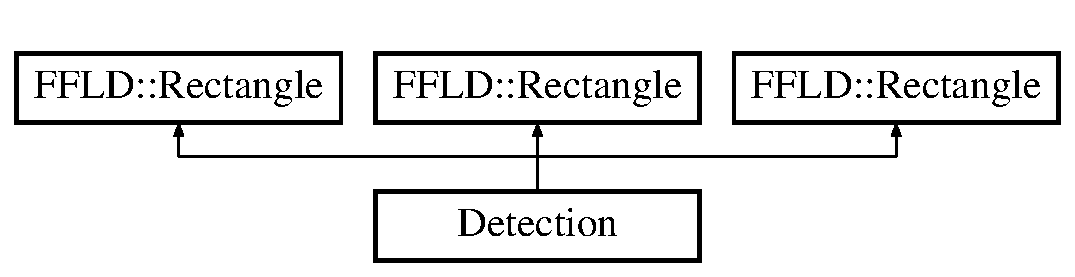
\includegraphics[height=2.000000cm]{struct_detection}
\end{center}
\end{figure}
\subsection*{Public Member Functions}
\begin{DoxyCompactItemize}
\item 
\hypertarget{struct_detection_a02c65365d9b9644cfc93afca0c03dc8b}{{\bfseries Detection} (\hyperlink{class_f_f_l_d_1_1_h_o_g_pyramid_af17c08ed86557e0a0aecb4814daf87c3}{H\-O\-G\-Pyramid\-::\-Scalar} score, int l, int x, int y, \hyperlink{class_f_f_l_d_1_1_rectangle}{F\-F\-L\-D\-::\-Rectangle} bndbox)}\label{struct_detection_a02c65365d9b9644cfc93afca0c03dc8b}

\item 
\hypertarget{struct_detection_a0664ad2933e1ae586236a9b575b2d496}{bool {\bfseries operator$<$} (const \hyperlink{struct_detection}{Detection} \&detection) const }\label{struct_detection_a0664ad2933e1ae586236a9b575b2d496}

\item 
\hypertarget{struct_detection_a02c65365d9b9644cfc93afca0c03dc8b}{{\bfseries Detection} (\hyperlink{class_f_f_l_d_1_1_h_o_g_pyramid_af17c08ed86557e0a0aecb4814daf87c3}{H\-O\-G\-Pyramid\-::\-Scalar} score, int l, int x, int y, \hyperlink{class_f_f_l_d_1_1_rectangle}{F\-F\-L\-D\-::\-Rectangle} bndbox)}\label{struct_detection_a02c65365d9b9644cfc93afca0c03dc8b}

\item 
\hypertarget{struct_detection_a0664ad2933e1ae586236a9b575b2d496}{bool {\bfseries operator$<$} (const \hyperlink{struct_detection}{Detection} \&detection) const }\label{struct_detection_a0664ad2933e1ae586236a9b575b2d496}

\item 
\hypertarget{struct_detection_a02c65365d9b9644cfc93afca0c03dc8b}{{\bfseries Detection} (\hyperlink{class_f_f_l_d_1_1_h_o_g_pyramid_af17c08ed86557e0a0aecb4814daf87c3}{H\-O\-G\-Pyramid\-::\-Scalar} score, int l, int x, int y, \hyperlink{class_f_f_l_d_1_1_rectangle}{F\-F\-L\-D\-::\-Rectangle} bndbox)}\label{struct_detection_a02c65365d9b9644cfc93afca0c03dc8b}

\item 
\hypertarget{struct_detection_a0664ad2933e1ae586236a9b575b2d496}{bool {\bfseries operator$<$} (const \hyperlink{struct_detection}{Detection} \&detection) const }\label{struct_detection_a0664ad2933e1ae586236a9b575b2d496}

\end{DoxyCompactItemize}
\subsection*{Public Attributes}
\begin{DoxyCompactItemize}
\item 
\hypertarget{struct_detection_a6bb0acb0597ec67b7049c2560c6c7783}{\hyperlink{class_f_f_l_d_1_1_h_o_g_pyramid_af17c08ed86557e0a0aecb4814daf87c3}{H\-O\-G\-Pyramid\-::\-Scalar} {\bfseries score}}\label{struct_detection_a6bb0acb0597ec67b7049c2560c6c7783}

\item 
\hypertarget{struct_detection_a08b01da4f3061254d1647bf737b172ed}{int {\bfseries l}}\label{struct_detection_a08b01da4f3061254d1647bf737b172ed}

\item 
\hypertarget{struct_detection_a7b71921325261514cd6dd42c8e90ba70}{int {\bfseries x}}\label{struct_detection_a7b71921325261514cd6dd42c8e90ba70}

\item 
\hypertarget{struct_detection_afa5d065ea13ce74dfd52c6a569313270}{int {\bfseries y}}\label{struct_detection_afa5d065ea13ce74dfd52c6a569313270}

\end{DoxyCompactItemize}


The documentation for this struct was generated from the following files\-:\begin{DoxyCompactItemize}
\item 
/\-Users/raphaeldendooven/\-Documents/school/2013-\/2014\-\_\-\-Thesis\-\_\-\-Master/\-Programs/\-Hand\-Detection/ffld2.\-cpp\item 
/\-Users/raphaeldendooven/\-Documents/school/2013-\/2014\-\_\-\-Thesis\-\_\-\-Master/\-Programs/\-Hand\-Detection/Person\-Detection.\-h\item 
/\-Users/raphaeldendooven/\-Documents/school/2013-\/2014\-\_\-\-Thesis\-\_\-\-Master/\-Programs/\-Hand\-Detection/Person\-Detection\-\_\-old.\-h\end{DoxyCompactItemize}

\hypertarget{class_det_hand}{\section{Det\-Hand Class Reference}
\label{class_det_hand}\index{Det\-Hand@{Det\-Hand}}
}


{\ttfamily \#include $<$Det\-Hand.\-h$>$}

\subsection*{Public Member Functions}
\begin{DoxyCompactItemize}
\item 
\hyperlink{class_det_hand_ae2db0bd3a42211dd7f85aa484163fb51}{Det\-Hand} (String model\-Hand, String context\-Model, double threshold)
\begin{DoxyCompactList}\small\item\em Constructor from classe \hyperlink{class_det_hand}{Det\-Hand}. Preps the detector with the right hand model. \end{DoxyCompactList}\item 
void \hyperlink{class_det_hand_a2ff6d2defe5cb9fb6d478a113dd07800}{run\-Detection} (Mat image, int frame\-Number, Rect face)
\begin{DoxyCompactList}\small\item\em Apply the detector on a image. \end{DoxyCompactList}\item 
void \hyperlink{class_det_hand_a04ca17b97c142aaeb4e687a3bcc23cd4}{draw\-Result} (Mat \&img, Rotated\-Rect \&box, const Scalar \&color)
\begin{DoxyCompactList}\small\item\em Draws the found regions on a image Draws a rotated rectangle with rescpect to the center. \end{DoxyCompactList}\item 
vector$<$ Mat $>$ \hyperlink{class_det_hand_afcb69946411c9c656f3203b6bbc4e13a}{get\-Cutouts} ()
\begin{DoxyCompactList}\small\item\em Get all the detection cutouts of the last detection. \end{DoxyCompactList}\item 
vector$<$ Rotated\-Rect $>$ \hyperlink{class_det_hand_a6d30403a8d530c2169b2ddbe5d5bdac6}{get\-Location\-Hand} ()
\begin{DoxyCompactList}\small\item\em Get the detection regions of the last detection with the respected rotation of the hand detector. \end{DoxyCompactList}\item 
vector$<$ double $>$ \hyperlink{class_det_hand_abb8015c29b1e4c6bf78ebe8bf87f49cd}{get\-Score\-Hand} ()
\begin{DoxyCompactList}\small\item\em Get score of hand detections found. \end{DoxyCompactList}\item 
vector$<$ Rotated\-Rect $>$ \hyperlink{class_det_hand_a22212d11ca6da3294e65a69d3438516c}{get\-Location\-Context} ()
\begin{DoxyCompactList}\small\item\em Get the detection regions of the last detection with the respected rotation of the context detector. \end{DoxyCompactList}\item 
vector$<$ double $>$ \hyperlink{class_det_hand_a66591d156dcb9ae702ec5bff58aff404}{get\-Score\-Context} ()
\begin{DoxyCompactList}\small\item\em Get score of context detections found. \end{DoxyCompactList}\item 
vector$<$ Rotated\-Rect $>$ \hyperlink{class_det_hand_a968add655757ec16229a217e6981ed1d}{get\-Location\-Arm} ()
\begin{DoxyCompactList}\small\item\em Get the detection regions of the last detection with the respected rotation of the arm hand detector. \end{DoxyCompactList}\item 
vector$<$ double $>$ \hyperlink{class_det_hand_aecc3b2a3541650dbbfeac38887ac1a61}{get\-Score\-Arm} ()
\begin{DoxyCompactList}\small\item\em Get score of arm detections found. \end{DoxyCompactList}\item 
Mat \hyperlink{class_det_hand_a0f824a1a3414cc612cbd475f901fd0b5}{get\-Skin} ()
\begin{DoxyCompactList}\small\item\em Get Skin segmentation. \end{DoxyCompactList}\end{DoxyCompactItemize}


\subsection{Detailed Description}
Hand detection class. Detects hand on images.

\begin{DoxyAuthor}{Author}
Den Dooven Raphael 
\end{DoxyAuthor}


\subsection{Constructor \& Destructor Documentation}
\hypertarget{class_det_hand_ae2db0bd3a42211dd7f85aa484163fb51}{\index{Det\-Hand@{Det\-Hand}!Det\-Hand@{Det\-Hand}}
\index{Det\-Hand@{Det\-Hand}!DetHand@{Det\-Hand}}
\subsubsection[{Det\-Hand}]{\setlength{\rightskip}{0pt plus 5cm}Det\-Hand\-::\-Det\-Hand (
\begin{DoxyParamCaption}
\item[{String}]{model\-Hand, }
\item[{String}]{context\-Model, }
\item[{double}]{threshold}
\end{DoxyParamCaption}
)}}\label{class_det_hand_ae2db0bd3a42211dd7f85aa484163fb51}


Constructor from classe \hyperlink{class_det_hand}{Det\-Hand}. Preps the detector with the right hand model. 


\begin{DoxyParams}{Parameters}
{\em Model\-Hand} & Filename of model \\
\hline
{\em threshold} & Threshold value of detector \\
\hline
\end{DoxyParams}


\subsection{Member Function Documentation}
\hypertarget{class_det_hand_a04ca17b97c142aaeb4e687a3bcc23cd4}{\index{Det\-Hand@{Det\-Hand}!draw\-Result@{draw\-Result}}
\index{draw\-Result@{draw\-Result}!DetHand@{Det\-Hand}}
\subsubsection[{draw\-Result}]{\setlength{\rightskip}{0pt plus 5cm}void Det\-Hand\-::draw\-Result (
\begin{DoxyParamCaption}
\item[{Mat \&}]{img, }
\item[{Rotated\-Rect \&}]{box, }
\item[{const Scalar \&}]{color}
\end{DoxyParamCaption}
)}}\label{class_det_hand_a04ca17b97c142aaeb4e687a3bcc23cd4}


Draws the found regions on a image Draws a rotated rectangle with rescpect to the center. 


\begin{DoxyParams}{Parameters}
{\em img} & Detination image \\
\hline
{\em box} & Rectangle information \\
\hline
{\em angle} & Rectangles rotation with rescpect to the center \\
\hline
{\em color} & color op the rectangle \\
\hline
\end{DoxyParams}
\hypertarget{class_det_hand_afcb69946411c9c656f3203b6bbc4e13a}{\index{Det\-Hand@{Det\-Hand}!get\-Cutouts@{get\-Cutouts}}
\index{get\-Cutouts@{get\-Cutouts}!DetHand@{Det\-Hand}}
\subsubsection[{get\-Cutouts}]{\setlength{\rightskip}{0pt plus 5cm}vector$<$Mat$>$ Det\-Hand\-::get\-Cutouts (
\begin{DoxyParamCaption}
{}
\end{DoxyParamCaption}
)}}\label{class_det_hand_afcb69946411c9c656f3203b6bbc4e13a}


Get all the detection cutouts of the last detection. 

\begin{DoxyReturn}{Returns}
All cutouts of type Mat put in a vector 
\end{DoxyReturn}
\hypertarget{class_det_hand_a968add655757ec16229a217e6981ed1d}{\index{Det\-Hand@{Det\-Hand}!get\-Location\-Arm@{get\-Location\-Arm}}
\index{get\-Location\-Arm@{get\-Location\-Arm}!DetHand@{Det\-Hand}}
\subsubsection[{get\-Location\-Arm}]{\setlength{\rightskip}{0pt plus 5cm}vector$<$ Rotated\-Rect $>$ Det\-Hand\-::get\-Location\-Arm (
\begin{DoxyParamCaption}
{}
\end{DoxyParamCaption}
)}}\label{class_det_hand_a968add655757ec16229a217e6981ed1d}


Get the detection regions of the last detection with the respected rotation of the arm hand detector. 

\begin{DoxyReturn}{Returns}
All regions of type Rect and rotation put in a vector 
\end{DoxyReturn}
\hypertarget{class_det_hand_a22212d11ca6da3294e65a69d3438516c}{\index{Det\-Hand@{Det\-Hand}!get\-Location\-Context@{get\-Location\-Context}}
\index{get\-Location\-Context@{get\-Location\-Context}!DetHand@{Det\-Hand}}
\subsubsection[{get\-Location\-Context}]{\setlength{\rightskip}{0pt plus 5cm}vector$<$ Rotated\-Rect $>$ Det\-Hand\-::get\-Location\-Context (
\begin{DoxyParamCaption}
{}
\end{DoxyParamCaption}
)}}\label{class_det_hand_a22212d11ca6da3294e65a69d3438516c}


Get the detection regions of the last detection with the respected rotation of the context detector. 

\begin{DoxyReturn}{Returns}
All regions of type Rect and rotation put in a vector 
\end{DoxyReturn}
\hypertarget{class_det_hand_a6d30403a8d530c2169b2ddbe5d5bdac6}{\index{Det\-Hand@{Det\-Hand}!get\-Location\-Hand@{get\-Location\-Hand}}
\index{get\-Location\-Hand@{get\-Location\-Hand}!DetHand@{Det\-Hand}}
\subsubsection[{get\-Location\-Hand}]{\setlength{\rightskip}{0pt plus 5cm}vector$<$ Rotated\-Rect $>$ Det\-Hand\-::get\-Location\-Hand (
\begin{DoxyParamCaption}
{}
\end{DoxyParamCaption}
)}}\label{class_det_hand_a6d30403a8d530c2169b2ddbe5d5bdac6}


Get the detection regions of the last detection with the respected rotation of the hand detector. 

\begin{DoxyReturn}{Returns}
All regions of type Rect and rotation put in a vector 
\end{DoxyReturn}
\hypertarget{class_det_hand_aecc3b2a3541650dbbfeac38887ac1a61}{\index{Det\-Hand@{Det\-Hand}!get\-Score\-Arm@{get\-Score\-Arm}}
\index{get\-Score\-Arm@{get\-Score\-Arm}!DetHand@{Det\-Hand}}
\subsubsection[{get\-Score\-Arm}]{\setlength{\rightskip}{0pt plus 5cm}vector$<$ double $>$ Det\-Hand\-::get\-Score\-Arm (
\begin{DoxyParamCaption}
{}
\end{DoxyParamCaption}
)}}\label{class_det_hand_aecc3b2a3541650dbbfeac38887ac1a61}


Get score of arm detections found. 

\begin{DoxyReturn}{Returns}
Score of detections found 
\end{DoxyReturn}
\hypertarget{class_det_hand_a66591d156dcb9ae702ec5bff58aff404}{\index{Det\-Hand@{Det\-Hand}!get\-Score\-Context@{get\-Score\-Context}}
\index{get\-Score\-Context@{get\-Score\-Context}!DetHand@{Det\-Hand}}
\subsubsection[{get\-Score\-Context}]{\setlength{\rightskip}{0pt plus 5cm}vector$<$ double $>$ Det\-Hand\-::get\-Score\-Context (
\begin{DoxyParamCaption}
{}
\end{DoxyParamCaption}
)}}\label{class_det_hand_a66591d156dcb9ae702ec5bff58aff404}


Get score of context detections found. 

\begin{DoxyReturn}{Returns}
Score of detections found 
\end{DoxyReturn}
\hypertarget{class_det_hand_abb8015c29b1e4c6bf78ebe8bf87f49cd}{\index{Det\-Hand@{Det\-Hand}!get\-Score\-Hand@{get\-Score\-Hand}}
\index{get\-Score\-Hand@{get\-Score\-Hand}!DetHand@{Det\-Hand}}
\subsubsection[{get\-Score\-Hand}]{\setlength{\rightskip}{0pt plus 5cm}vector$<$ double $>$ Det\-Hand\-::get\-Score\-Hand (
\begin{DoxyParamCaption}
{}
\end{DoxyParamCaption}
)}}\label{class_det_hand_abb8015c29b1e4c6bf78ebe8bf87f49cd}


Get score of hand detections found. 

\begin{DoxyReturn}{Returns}
Score of detections found 
\end{DoxyReturn}
\hypertarget{class_det_hand_a0f824a1a3414cc612cbd475f901fd0b5}{\index{Det\-Hand@{Det\-Hand}!get\-Skin@{get\-Skin}}
\index{get\-Skin@{get\-Skin}!DetHand@{Det\-Hand}}
\subsubsection[{get\-Skin}]{\setlength{\rightskip}{0pt plus 5cm}Mat Det\-Hand\-::get\-Skin (
\begin{DoxyParamCaption}
{}
\end{DoxyParamCaption}
)}}\label{class_det_hand_a0f824a1a3414cc612cbd475f901fd0b5}


Get Skin segmentation. 

\begin{DoxyReturn}{Returns}
skin 
\end{DoxyReturn}
\hypertarget{class_det_hand_a2ff6d2defe5cb9fb6d478a113dd07800}{\index{Det\-Hand@{Det\-Hand}!run\-Detection@{run\-Detection}}
\index{run\-Detection@{run\-Detection}!DetHand@{Det\-Hand}}
\subsubsection[{run\-Detection}]{\setlength{\rightskip}{0pt plus 5cm}void Det\-Hand\-::run\-Detection (
\begin{DoxyParamCaption}
\item[{Mat}]{image, }
\item[{int}]{frame\-Number, }
\item[{Rect}]{face}
\end{DoxyParamCaption}
)}}\label{class_det_hand_a2ff6d2defe5cb9fb6d478a113dd07800}


Apply the detector on a image. 


\begin{DoxyParams}{Parameters}
{\em image} & The image for the detector \\
\hline
{\em framenumber} & Frame number of the video (not really importend) \\
\hline
{\em face} & Give location face for skin segmentation \\
\hline
\end{DoxyParams}


The documentation for this class was generated from the following files\-:\begin{DoxyCompactItemize}
\item 
/\-Users/raphaeldendooven/\-Documents/school/2013-\/2014\-\_\-\-Thesis\-\_\-\-Master/\-Programs/\-Hand\-Detection/Det\-Hand.\-h\item 
/\-Users/raphaeldendooven/\-Documents/school/2013-\/2014\-\_\-\-Thesis\-\_\-\-Master/\-Programs/\-Hand\-Detection/Det\-Hand.\-cpp\end{DoxyCompactItemize}

\input{class_face_detection}
\input{class_highest_likelihood}
\hypertarget{class_f_f_l_d_1_1_h_o_g_pyramid}{\section{F\-F\-L\-D\-:\-:H\-O\-G\-Pyramid Class Reference}
\label{class_f_f_l_d_1_1_h_o_g_pyramid}\index{F\-F\-L\-D\-::\-H\-O\-G\-Pyramid@{F\-F\-L\-D\-::\-H\-O\-G\-Pyramid}}
}


{\ttfamily \#include $<$H\-O\-G\-Pyramid.\-h$>$}

\subsection*{Public Types}
\begin{DoxyCompactItemize}
\item 
\hypertarget{class_f_f_l_d_1_1_h_o_g_pyramid_af17c08ed86557e0a0aecb4814daf87c3}{typedef float \hyperlink{class_f_f_l_d_1_1_h_o_g_pyramid_af17c08ed86557e0a0aecb4814daf87c3}{Scalar}}\label{class_f_f_l_d_1_1_h_o_g_pyramid_af17c08ed86557e0a0aecb4814daf87c3}

\begin{DoxyCompactList}\small\item\em Type of a scalar value. \end{DoxyCompactList}\item 
\hypertarget{class_f_f_l_d_1_1_h_o_g_pyramid_a2618b4bd5d17f05cdc108189ed5abe3a}{typedef Eigen\-::\-Matrix$<$ \hyperlink{class_f_f_l_d_1_1_h_o_g_pyramid_af17c08ed86557e0a0aecb4814daf87c3}{Scalar}, \\*
Eigen\-::\-Dynamic, Eigen\-::\-Dynamic, \\*
Eigen\-::\-Row\-Major $>$ \hyperlink{class_f_f_l_d_1_1_h_o_g_pyramid_a2618b4bd5d17f05cdc108189ed5abe3a}{Matrix}}\label{class_f_f_l_d_1_1_h_o_g_pyramid_a2618b4bd5d17f05cdc108189ed5abe3a}

\begin{DoxyCompactList}\small\item\em Type of a matrix. \end{DoxyCompactList}\item 
\hypertarget{class_f_f_l_d_1_1_h_o_g_pyramid_a7f1784cd0a524bd5a2ecdd6e0dc98c35}{typedef Eigen\-::\-Sparse\-Matrix\\*
$<$ \hyperlink{class_f_f_l_d_1_1_h_o_g_pyramid_af17c08ed86557e0a0aecb4814daf87c3}{Scalar}, Eigen\-::\-Row\-Major $>$ \hyperlink{class_f_f_l_d_1_1_h_o_g_pyramid_a7f1784cd0a524bd5a2ecdd6e0dc98c35}{Sparse\-Matrix}}\label{class_f_f_l_d_1_1_h_o_g_pyramid_a7f1784cd0a524bd5a2ecdd6e0dc98c35}

\begin{DoxyCompactList}\small\item\em Type of a sparse matrix. \end{DoxyCompactList}\item 
\hypertarget{class_f_f_l_d_1_1_h_o_g_pyramid_a4d44ca52d8c41e79d36ddd6f2982ea1a}{typedef Eigen\-::\-Array$<$ \hyperlink{class_f_f_l_d_1_1_h_o_g_pyramid_af17c08ed86557e0a0aecb4814daf87c3}{Scalar}, \\*
\hyperlink{class_f_f_l_d_1_1_h_o_g_pyramid_a418ebc8cf8781a3874f50b5eac482c68}{Nb\-Features}, 1 $>$ \hyperlink{class_f_f_l_d_1_1_h_o_g_pyramid_a4d44ca52d8c41e79d36ddd6f2982ea1a}{Cell}}\label{class_f_f_l_d_1_1_h_o_g_pyramid_a4d44ca52d8c41e79d36ddd6f2982ea1a}

\begin{DoxyCompactList}\small\item\em Type of a pyramid level cell (fixed-\/size vector of length Nb\-Features). \end{DoxyCompactList}\item 
\hypertarget{class_f_f_l_d_1_1_h_o_g_pyramid_a1cd36670adf29538f44dfa434695ec34}{typedef Eigen\-::\-Matrix$<$ \hyperlink{class_f_f_l_d_1_1_h_o_g_pyramid_a4d44ca52d8c41e79d36ddd6f2982ea1a}{Cell}, \\*
Eigen\-::\-Dynamic, Eigen\-::\-Dynamic, \\*
Eigen\-::\-Row\-Major $>$ \hyperlink{class_f_f_l_d_1_1_h_o_g_pyramid_a1cd36670adf29538f44dfa434695ec34}{Level}}\label{class_f_f_l_d_1_1_h_o_g_pyramid_a1cd36670adf29538f44dfa434695ec34}

\begin{DoxyCompactList}\small\item\em Type of a pyramid level (matrix of cells). \end{DoxyCompactList}\end{DoxyCompactItemize}
\subsection*{Public Member Functions}
\begin{DoxyCompactItemize}
\item 
\hypertarget{class_f_f_l_d_1_1_h_o_g_pyramid_aab86c8da61b9ea188deab320c692a375}{\hyperlink{class_f_f_l_d_1_1_h_o_g_pyramid_aab86c8da61b9ea188deab320c692a375}{H\-O\-G\-Pyramid} ()}\label{class_f_f_l_d_1_1_h_o_g_pyramid_aab86c8da61b9ea188deab320c692a375}

\begin{DoxyCompactList}\small\item\em Constructs an empty pyramid. An empty pyramid has no level. \end{DoxyCompactList}\item 
\hyperlink{class_f_f_l_d_1_1_h_o_g_pyramid_a951d92ffa66b7e7d9d5fe44209fcaf26}{H\-O\-G\-Pyramid} (int \hyperlink{class_f_f_l_d_1_1_h_o_g_pyramid_aa8ed24222e8a5bd45374bc91451614cc}{padx}, int \hyperlink{class_f_f_l_d_1_1_h_o_g_pyramid_a4f29cae69e366eb3b5c36b0bdde6962f}{pady}, int \hyperlink{class_f_f_l_d_1_1_h_o_g_pyramid_a86c9ee51bac62aa0bd7fe8b29ad32cab}{interval}, const std\-::vector$<$ \hyperlink{class_f_f_l_d_1_1_h_o_g_pyramid_a1cd36670adf29538f44dfa434695ec34}{Level} $>$ \&\hyperlink{class_f_f_l_d_1_1_h_o_g_pyramid_ad43fe5cba5e0f23c0741a15b43da9079}{levels})
\item 
\hyperlink{class_f_f_l_d_1_1_h_o_g_pyramid_a64d8016358e951b1953cbcc8605c586f}{H\-O\-G\-Pyramid} (const \hyperlink{class_f_f_l_d_1_1_j_p_e_g_image}{J\-P\-E\-G\-Image} \&image, int \hyperlink{class_f_f_l_d_1_1_h_o_g_pyramid_aa8ed24222e8a5bd45374bc91451614cc}{padx}, int \hyperlink{class_f_f_l_d_1_1_h_o_g_pyramid_a4f29cae69e366eb3b5c36b0bdde6962f}{pady}, int \hyperlink{class_f_f_l_d_1_1_h_o_g_pyramid_a86c9ee51bac62aa0bd7fe8b29ad32cab}{interval}=10)
\item 
\hypertarget{class_f_f_l_d_1_1_h_o_g_pyramid_a5cb91dd6aee4788f68e25d565bca95de}{bool \hyperlink{class_f_f_l_d_1_1_h_o_g_pyramid_a5cb91dd6aee4788f68e25d565bca95de}{empty} () const }\label{class_f_f_l_d_1_1_h_o_g_pyramid_a5cb91dd6aee4788f68e25d565bca95de}

\begin{DoxyCompactList}\small\item\em Returns whether the pyramid is empty. An empty pyramid has no level. \end{DoxyCompactList}\item 
\hypertarget{class_f_f_l_d_1_1_h_o_g_pyramid_aa8ed24222e8a5bd45374bc91451614cc}{int \hyperlink{class_f_f_l_d_1_1_h_o_g_pyramid_aa8ed24222e8a5bd45374bc91451614cc}{padx} () const }\label{class_f_f_l_d_1_1_h_o_g_pyramid_aa8ed24222e8a5bd45374bc91451614cc}

\begin{DoxyCompactList}\small\item\em Returns the amount of horizontal zero padding (in cells). \end{DoxyCompactList}\item 
\hypertarget{class_f_f_l_d_1_1_h_o_g_pyramid_a4f29cae69e366eb3b5c36b0bdde6962f}{int \hyperlink{class_f_f_l_d_1_1_h_o_g_pyramid_a4f29cae69e366eb3b5c36b0bdde6962f}{pady} () const }\label{class_f_f_l_d_1_1_h_o_g_pyramid_a4f29cae69e366eb3b5c36b0bdde6962f}

\begin{DoxyCompactList}\small\item\em Returns the amount of vertical zero padding (in cells). \end{DoxyCompactList}\item 
\hypertarget{class_f_f_l_d_1_1_h_o_g_pyramid_a86c9ee51bac62aa0bd7fe8b29ad32cab}{int \hyperlink{class_f_f_l_d_1_1_h_o_g_pyramid_a86c9ee51bac62aa0bd7fe8b29ad32cab}{interval} () const }\label{class_f_f_l_d_1_1_h_o_g_pyramid_a86c9ee51bac62aa0bd7fe8b29ad32cab}

\begin{DoxyCompactList}\small\item\em Returns the number of levels per octave in the pyramid. \end{DoxyCompactList}\item 
const std\-::vector$<$ \hyperlink{class_f_f_l_d_1_1_h_o_g_pyramid_a1cd36670adf29538f44dfa434695ec34}{Level} $>$ \& \hyperlink{class_f_f_l_d_1_1_h_o_g_pyramid_ad43fe5cba5e0f23c0741a15b43da9079}{levels} () const 
\item 
void \hyperlink{class_f_f_l_d_1_1_h_o_g_pyramid_a90bcd58cf1dd4a47d128d2135b077c8c}{convolve} (const \hyperlink{class_f_f_l_d_1_1_h_o_g_pyramid_a1cd36670adf29538f44dfa434695ec34}{Level} \&filter, std\-::vector$<$ \hyperlink{class_f_f_l_d_1_1_h_o_g_pyramid_a2618b4bd5d17f05cdc108189ed5abe3a}{Matrix} $>$ \&convolutions) const 
\item 
void \hyperlink{class_f_f_l_d_1_1_h_o_g_pyramid_a55ebcb020dfece07f3e806ccbb4ad3c9}{convolve} (const \hyperlink{class_f_f_l_d_1_1_h_o_g_pyramid_a1cd36670adf29538f44dfa434695ec34}{Level} \&filter, std\-::vector$<$ \hyperlink{class_f_f_l_d_1_1_h_o_g_pyramid_a7f1784cd0a524bd5a2ecdd6e0dc98c35}{Sparse\-Matrix} $>$ \&convolutions) const 
\item 
void \hyperlink{class_f_f_l_d_1_1_h_o_g_pyramid_a0a90c310f6e1ccdb2c02374caa0f8de7}{convolve} (const std\-::vector$<$ \hyperlink{class_f_f_l_d_1_1_h_o_g_pyramid_a2618b4bd5d17f05cdc108189ed5abe3a}{Matrix} $>$ \&labels, \hyperlink{class_f_f_l_d_1_1_h_o_g_pyramid_a1cd36670adf29538f44dfa434695ec34}{Level} \&sum) const 
\item 
void \hyperlink{class_f_f_l_d_1_1_h_o_g_pyramid_a63793871ef3cd2a25312159561ede09c}{convolve} (const std\-::vector$<$ \hyperlink{class_f_f_l_d_1_1_h_o_g_pyramid_a7f1784cd0a524bd5a2ecdd6e0dc98c35}{Sparse\-Matrix} $>$ \&labels, \hyperlink{class_f_f_l_d_1_1_h_o_g_pyramid_a1cd36670adf29538f44dfa434695ec34}{Level} \&sum) const 
\end{DoxyCompactItemize}
\subsection*{Static Public Member Functions}
\begin{DoxyCompactItemize}
\item 
static Eigen\-::\-Map$<$ \hyperlink{class_f_f_l_d_1_1_h_o_g_pyramid_a2618b4bd5d17f05cdc108189ed5abe3a}{Matrix}, \\*
Eigen\-::\-Aligned $>$ \hyperlink{class_f_f_l_d_1_1_h_o_g_pyramid_a95908d95147f370b708886757f2a761d}{Convert} (\hyperlink{class_f_f_l_d_1_1_h_o_g_pyramid_a1cd36670adf29538f44dfa434695ec34}{Level} \&level)
\item 
static Eigen\-::\-Map$<$ const \\*
\hyperlink{class_f_f_l_d_1_1_h_o_g_pyramid_a2618b4bd5d17f05cdc108189ed5abe3a}{Matrix}, Eigen\-::\-Aligned $>$ \hyperlink{class_f_f_l_d_1_1_h_o_g_pyramid_a362ffc5ea00d23021947666ffb55060c}{Convert} (const \hyperlink{class_f_f_l_d_1_1_h_o_g_pyramid_a1cd36670adf29538f44dfa434695ec34}{Level} \&level)
\item 
\hypertarget{class_f_f_l_d_1_1_h_o_g_pyramid_aec98ef9669e289f2aa30235fdbe0df87}{static \hyperlink{class_f_f_l_d_1_1_h_o_g_pyramid_a1cd36670adf29538f44dfa434695ec34}{H\-O\-G\-Pyramid\-::\-Level} \hyperlink{class_f_f_l_d_1_1_h_o_g_pyramid_aec98ef9669e289f2aa30235fdbe0df87}{Flip} (const \hyperlink{class_f_f_l_d_1_1_h_o_g_pyramid_a1cd36670adf29538f44dfa434695ec34}{H\-O\-G\-Pyramid\-::\-Level} \&filter)}\label{class_f_f_l_d_1_1_h_o_g_pyramid_aec98ef9669e289f2aa30235fdbe0df87}

\begin{DoxyCompactList}\small\item\em Returns the flipped version (horizontally) of a filter. \end{DoxyCompactList}\end{DoxyCompactItemize}
\subsection*{Static Public Attributes}
\begin{DoxyCompactItemize}
\item 
static const int \hyperlink{class_f_f_l_d_1_1_h_o_g_pyramid_a418ebc8cf8781a3874f50b5eac482c68}{Nb\-Features} = 32
\end{DoxyCompactItemize}


\subsection{Detailed Description}
The \hyperlink{class_f_f_l_d_1_1_h_o_g_pyramid}{H\-O\-G\-Pyramid} class computes and stores the H\-O\-G features extracted from a jpeg image at multiple scales. The scale of the pyramid level of index {\ttfamily i} is given by the following formula\-: 2$^\wedge$(1 -\/ {\ttfamily i} / {\ttfamily interval}), so that the first scale is at double the resolution of the original image). Each level is padded with zeros horizontally and vertically by a fixed amount. The last feature is special\-: it takes the value one in the padding and zero otherwise. \begin{DoxyNote}{Note}
Define the P\-A\-S\-C\-A\-L\-\_\-\-H\-O\-G\-P\-Y\-R\-A\-M\-I\-D\-\_\-\-F\-E\-L\-Z\-E\-N\-S\-Z\-W\-A\-L\-B\-\_\-\-F\-E\-A\-T\-U\-R\-E\-S flag during compilation to use Felzenszwalb's original features (slower and not as accurate as they do no angular interpolation, provided for compatibility only). 

Define the P\-A\-S\-C\-A\-L\-\_\-\-H\-O\-G\-P\-Y\-R\-A\-M\-I\-D\-\_\-\-D\-O\-U\-B\-L\-E to use double scalar values instead of float (slower, uses twice the amount of memory, and the increase in precision is not necessarily useful). 
\end{DoxyNote}


\subsection{Constructor \& Destructor Documentation}
\hypertarget{class_f_f_l_d_1_1_h_o_g_pyramid_a951d92ffa66b7e7d9d5fe44209fcaf26}{\index{F\-F\-L\-D\-::\-H\-O\-G\-Pyramid@{F\-F\-L\-D\-::\-H\-O\-G\-Pyramid}!H\-O\-G\-Pyramid@{H\-O\-G\-Pyramid}}
\index{H\-O\-G\-Pyramid@{H\-O\-G\-Pyramid}!FFLD::HOGPyramid@{F\-F\-L\-D\-::\-H\-O\-G\-Pyramid}}
\subsubsection[{H\-O\-G\-Pyramid}]{\setlength{\rightskip}{0pt plus 5cm}F\-F\-L\-D\-::\-H\-O\-G\-Pyramid\-::\-H\-O\-G\-Pyramid (
\begin{DoxyParamCaption}
\item[{int}]{padx, }
\item[{int}]{pady, }
\item[{int}]{interval, }
\item[{const std\-::vector$<$ {\bf Level} $>$ \&}]{levels}
\end{DoxyParamCaption}
)}}\label{class_f_f_l_d_1_1_h_o_g_pyramid_a951d92ffa66b7e7d9d5fe44209fcaf26}
Constructs a pyramid from parameters and a list of levels. 
\begin{DoxyParams}[1]{Parameters}
\mbox{\tt in}  & {\em padx} & Amount of horizontal zero padding (in cells). \\
\hline
\mbox{\tt in}  & {\em pady} & Amount of vertical zero padding (in cells). \\
\hline
\mbox{\tt in}  & {\em interval} & Number of levels per octave in the pyramid. \\
\hline
\mbox{\tt in}  & {\em levels} & List of pyramid levels. \\
\hline
\end{DoxyParams}
\begin{DoxyNote}{Note}
The amount of padding and the interval should be at least 1. 
\end{DoxyNote}
\hypertarget{class_f_f_l_d_1_1_h_o_g_pyramid_a64d8016358e951b1953cbcc8605c586f}{\index{F\-F\-L\-D\-::\-H\-O\-G\-Pyramid@{F\-F\-L\-D\-::\-H\-O\-G\-Pyramid}!H\-O\-G\-Pyramid@{H\-O\-G\-Pyramid}}
\index{H\-O\-G\-Pyramid@{H\-O\-G\-Pyramid}!FFLD::HOGPyramid@{F\-F\-L\-D\-::\-H\-O\-G\-Pyramid}}
\subsubsection[{H\-O\-G\-Pyramid}]{\setlength{\rightskip}{0pt plus 5cm}H\-O\-G\-Pyramid\-::\-H\-O\-G\-Pyramid (
\begin{DoxyParamCaption}
\item[{const {\bf J\-P\-E\-G\-Image} \&}]{image, }
\item[{int}]{padx, }
\item[{int}]{pady, }
\item[{int}]{interval = {\ttfamily 10}}
\end{DoxyParamCaption}
)}}\label{class_f_f_l_d_1_1_h_o_g_pyramid_a64d8016358e951b1953cbcc8605c586f}
Constructs a pyramid from the \hyperlink{class_f_f_l_d_1_1_j_p_e_g_image}{J\-P\-E\-G\-Image} of a \hyperlink{class_f_f_l_d_1_1_scene}{Scene}. 
\begin{DoxyParams}[1]{Parameters}
\mbox{\tt in}  & {\em image} & The \hyperlink{class_f_f_l_d_1_1_j_p_e_g_image}{J\-P\-E\-G\-Image} of the \hyperlink{class_f_f_l_d_1_1_scene}{Scene}. \\
\hline
\mbox{\tt in}  & {\em padx} & Amount of horizontal zero padding (in cells). \\
\hline
\mbox{\tt in}  & {\em pady} & Amount of vertical zero padding (in cells). \\
\hline
\mbox{\tt in}  & {\em interval} & Number of levels per octave in the pyramid. \\
\hline
\end{DoxyParams}
\begin{DoxyNote}{Note}
The amount of padding and the interval should be at least 1. 
\end{DoxyNote}


\subsection{Member Function Documentation}
\hypertarget{class_f_f_l_d_1_1_h_o_g_pyramid_a95908d95147f370b708886757f2a761d}{\index{F\-F\-L\-D\-::\-H\-O\-G\-Pyramid@{F\-F\-L\-D\-::\-H\-O\-G\-Pyramid}!Convert@{Convert}}
\index{Convert@{Convert}!FFLD::HOGPyramid@{F\-F\-L\-D\-::\-H\-O\-G\-Pyramid}}
\subsubsection[{Convert}]{\setlength{\rightskip}{0pt plus 5cm}Map$<$ {\bf H\-O\-G\-Pyramid\-::\-Matrix}, Aligned $>$ H\-O\-G\-Pyramid\-::\-Convert (
\begin{DoxyParamCaption}
\item[{{\bf Level} \&}]{level}
\end{DoxyParamCaption}
)\hspace{0.3cm}{\ttfamily [static]}}}\label{class_f_f_l_d_1_1_h_o_g_pyramid_a95908d95147f370b708886757f2a761d}
Converts a pyramid level to a simple matrix (useful to apply standard matrix operations to it). \begin{DoxyNote}{Note}
The size of the matrix will be rows x (cols $\ast$ Nb\-Features). 
\end{DoxyNote}
\hypertarget{class_f_f_l_d_1_1_h_o_g_pyramid_a362ffc5ea00d23021947666ffb55060c}{\index{F\-F\-L\-D\-::\-H\-O\-G\-Pyramid@{F\-F\-L\-D\-::\-H\-O\-G\-Pyramid}!Convert@{Convert}}
\index{Convert@{Convert}!FFLD::HOGPyramid@{F\-F\-L\-D\-::\-H\-O\-G\-Pyramid}}
\subsubsection[{Convert}]{\setlength{\rightskip}{0pt plus 5cm}Map$<$ const {\bf H\-O\-G\-Pyramid\-::\-Matrix}, Aligned $>$ H\-O\-G\-Pyramid\-::\-Convert (
\begin{DoxyParamCaption}
\item[{const {\bf Level} \&}]{level}
\end{DoxyParamCaption}
)\hspace{0.3cm}{\ttfamily [static]}}}\label{class_f_f_l_d_1_1_h_o_g_pyramid_a362ffc5ea00d23021947666ffb55060c}
Converts a const pyramid level to a simple const matrix (useful to apply standard matrix operations to it). \begin{DoxyNote}{Note}
The size of the matrix will be rows x (cols $\ast$ Nb\-Features). 
\end{DoxyNote}
\hypertarget{class_f_f_l_d_1_1_h_o_g_pyramid_a90bcd58cf1dd4a47d128d2135b077c8c}{\index{F\-F\-L\-D\-::\-H\-O\-G\-Pyramid@{F\-F\-L\-D\-::\-H\-O\-G\-Pyramid}!convolve@{convolve}}
\index{convolve@{convolve}!FFLD::HOGPyramid@{F\-F\-L\-D\-::\-H\-O\-G\-Pyramid}}
\subsubsection[{convolve}]{\setlength{\rightskip}{0pt plus 5cm}void F\-F\-L\-D\-::\-H\-O\-G\-Pyramid\-::convolve (
\begin{DoxyParamCaption}
\item[{const {\bf Level} \&}]{filter, }
\item[{std\-::vector$<$ {\bf Matrix} $>$ \&}]{convolutions}
\end{DoxyParamCaption}
) const}}\label{class_f_f_l_d_1_1_h_o_g_pyramid_a90bcd58cf1dd4a47d128d2135b077c8c}
Returns the convolutions of the pyramid with a filter (useful to compute the S\-V\-M margins). 
\begin{DoxyParams}[1]{Parameters}
\mbox{\tt in}  & {\em filter} & Filter. \\
\hline
\mbox{\tt out}  & {\em convolutions} & Convolution for each level. \\
\hline
\end{DoxyParams}
\hypertarget{class_f_f_l_d_1_1_h_o_g_pyramid_a55ebcb020dfece07f3e806ccbb4ad3c9}{\index{F\-F\-L\-D\-::\-H\-O\-G\-Pyramid@{F\-F\-L\-D\-::\-H\-O\-G\-Pyramid}!convolve@{convolve}}
\index{convolve@{convolve}!FFLD::HOGPyramid@{F\-F\-L\-D\-::\-H\-O\-G\-Pyramid}}
\subsubsection[{convolve}]{\setlength{\rightskip}{0pt plus 5cm}void F\-F\-L\-D\-::\-H\-O\-G\-Pyramid\-::convolve (
\begin{DoxyParamCaption}
\item[{const {\bf Level} \&}]{filter, }
\item[{std\-::vector$<$ {\bf Sparse\-Matrix} $>$ \&}]{convolutions}
\end{DoxyParamCaption}
) const}}\label{class_f_f_l_d_1_1_h_o_g_pyramid_a55ebcb020dfece07f3e806ccbb4ad3c9}
Returns the sparse convolutions of the pyramid with a filter (useful to compute a subset of the S\-V\-M margins). 
\begin{DoxyParams}[1]{Parameters}
\mbox{\tt in}  & {\em filter} & The filter. \\
\hline
\mbox{\tt out}  & {\em convolutions} & The results of the convolutions for each level. \\
\hline
\end{DoxyParams}
\hypertarget{class_f_f_l_d_1_1_h_o_g_pyramid_a0a90c310f6e1ccdb2c02374caa0f8de7}{\index{F\-F\-L\-D\-::\-H\-O\-G\-Pyramid@{F\-F\-L\-D\-::\-H\-O\-G\-Pyramid}!convolve@{convolve}}
\index{convolve@{convolve}!FFLD::HOGPyramid@{F\-F\-L\-D\-::\-H\-O\-G\-Pyramid}}
\subsubsection[{convolve}]{\setlength{\rightskip}{0pt plus 5cm}void F\-F\-L\-D\-::\-H\-O\-G\-Pyramid\-::convolve (
\begin{DoxyParamCaption}
\item[{const std\-::vector$<$ {\bf Matrix} $>$ \&}]{labels, }
\item[{{\bf Level} \&}]{sum}
\end{DoxyParamCaption}
) const}}\label{class_f_f_l_d_1_1_h_o_g_pyramid_a0a90c310f6e1ccdb2c02374caa0f8de7}
Returns the sum of the convolutions of the pyramid with a pyramid of labels (useful to compute the gradient of the S\-V\-M loss). 
\begin{DoxyParams}[1]{Parameters}
\mbox{\tt in}  & {\em labels} & The pyramid of labels. \\
\hline
\mbox{\tt out}  & {\em sum} & The sum of the results of the convolutions. \\
\hline
\end{DoxyParams}
\begin{DoxyNote}{Note}
The size of the sum is inferred from the size of the labels, which should thus all have the size of their corresponding level minus the size of the sum plus one. 

In case labels are empty the sum will be empty too. 
\end{DoxyNote}
\hypertarget{class_f_f_l_d_1_1_h_o_g_pyramid_a63793871ef3cd2a25312159561ede09c}{\index{F\-F\-L\-D\-::\-H\-O\-G\-Pyramid@{F\-F\-L\-D\-::\-H\-O\-G\-Pyramid}!convolve@{convolve}}
\index{convolve@{convolve}!FFLD::HOGPyramid@{F\-F\-L\-D\-::\-H\-O\-G\-Pyramid}}
\subsubsection[{convolve}]{\setlength{\rightskip}{0pt plus 5cm}void F\-F\-L\-D\-::\-H\-O\-G\-Pyramid\-::convolve (
\begin{DoxyParamCaption}
\item[{const std\-::vector$<$ {\bf Sparse\-Matrix} $>$ \&}]{labels, }
\item[{{\bf Level} \&}]{sum}
\end{DoxyParamCaption}
) const}}\label{class_f_f_l_d_1_1_h_o_g_pyramid_a63793871ef3cd2a25312159561ede09c}
Returns the sum of the sparse convolutions of the pyramid with a pyramid of labels (useful to compute the gradient of the S\-V\-M loss). 
\begin{DoxyParams}[1]{Parameters}
\mbox{\tt in}  & {\em labels} & The pyramid of labels. \\
\hline
\mbox{\tt out}  & {\em sum} & The sum of the results of the convolutions. \\
\hline
\end{DoxyParams}
\begin{DoxyNote}{Note}
The size of the sum is inferred from the size of the labels, which should thus all have the size of their corresponding level minus the size of the sum plus one. 

In case labels are empty the sum will be empty too. 
\end{DoxyNote}
\hypertarget{class_f_f_l_d_1_1_h_o_g_pyramid_ad43fe5cba5e0f23c0741a15b43da9079}{\index{F\-F\-L\-D\-::\-H\-O\-G\-Pyramid@{F\-F\-L\-D\-::\-H\-O\-G\-Pyramid}!levels@{levels}}
\index{levels@{levels}!FFLD::HOGPyramid@{F\-F\-L\-D\-::\-H\-O\-G\-Pyramid}}
\subsubsection[{levels}]{\setlength{\rightskip}{0pt plus 5cm}const vector$<$ {\bf H\-O\-G\-Pyramid\-::\-Level} $>$ \& H\-O\-G\-Pyramid\-::levels (
\begin{DoxyParamCaption}
{}
\end{DoxyParamCaption}
) const}}\label{class_f_f_l_d_1_1_h_o_g_pyramid_ad43fe5cba5e0f23c0741a15b43da9079}
Returns the pyramid levels. \begin{DoxyNote}{Note}
Scales are given by the following formula\-: 2$^\wedge$(1 -\/ {\ttfamily index} / {\ttfamily interval}). 
\end{DoxyNote}


\subsection{Member Data Documentation}
\hypertarget{class_f_f_l_d_1_1_h_o_g_pyramid_a418ebc8cf8781a3874f50b5eac482c68}{\index{F\-F\-L\-D\-::\-H\-O\-G\-Pyramid@{F\-F\-L\-D\-::\-H\-O\-G\-Pyramid}!Nb\-Features@{Nb\-Features}}
\index{Nb\-Features@{Nb\-Features}!FFLD::HOGPyramid@{F\-F\-L\-D\-::\-H\-O\-G\-Pyramid}}
\subsubsection[{Nb\-Features}]{\setlength{\rightskip}{0pt plus 5cm}const int F\-F\-L\-D\-::\-H\-O\-G\-Pyramid\-::\-Nb\-Features = 32\hspace{0.3cm}{\ttfamily [static]}}}\label{class_f_f_l_d_1_1_h_o_g_pyramid_a418ebc8cf8781a3874f50b5eac482c68}
Number of H\-O\-G features (guaranteed to be even). Fixed at compile time for both ease of use and optimal performance. 

The documentation for this class was generated from the following files\-:\begin{DoxyCompactItemize}
\item 
H\-O\-G\-Pyramid.\-h\item 
H\-O\-G\-Pyramid.\-cpp\end{DoxyCompactItemize}

\hypertarget{class_f_f_l_d_1_1_intersector}{\section{F\-F\-L\-D\-:\-:Intersector Class Reference}
\label{class_f_f_l_d_1_1_intersector}\index{F\-F\-L\-D\-::\-Intersector@{F\-F\-L\-D\-::\-Intersector}}
}


{\ttfamily \#include $<$Intersector.\-h$>$}

\subsection*{Public Member Functions}
\begin{DoxyCompactItemize}
\item 
\hyperlink{class_f_f_l_d_1_1_intersector_aed95bdbcf7b5f24b1dd5b797bcc127fd}{Intersector} (\hyperlink{class_f_f_l_d_1_1_rectangle}{Rectangle} reference, double threshold=0.\-5, bool felzenszwalb=false)
\item 
bool \hyperlink{class_f_f_l_d_1_1_intersector_a2ba78e41d3bf04a2ced101d56ad47d85}{operator()} (\hyperlink{class_f_f_l_d_1_1_rectangle}{Rectangle} rect, double $\ast$score=0) const 
\end{DoxyCompactItemize}


\subsection{Detailed Description}
Functor used to test for the intersection of two rectangles according to the Pascal criterion (area of intersection over area of union). 

\subsection{Constructor \& Destructor Documentation}
\hypertarget{class_f_f_l_d_1_1_intersector_aed95bdbcf7b5f24b1dd5b797bcc127fd}{\index{F\-F\-L\-D\-::\-Intersector@{F\-F\-L\-D\-::\-Intersector}!Intersector@{Intersector}}
\index{Intersector@{Intersector}!FFLD::Intersector@{F\-F\-L\-D\-::\-Intersector}}
\subsubsection[{Intersector}]{\setlength{\rightskip}{0pt plus 5cm}F\-F\-L\-D\-::\-Intersector\-::\-Intersector (
\begin{DoxyParamCaption}
\item[{{\bf Rectangle}}]{reference, }
\item[{double}]{threshold = {\ttfamily 0.5}, }
\item[{bool}]{felzenszwalb = {\ttfamily false}}
\end{DoxyParamCaption}
)\hspace{0.3cm}{\ttfamily [inline]}}}\label{class_f_f_l_d_1_1_intersector_aed95bdbcf7b5f24b1dd5b797bcc127fd}
Constructor. 
\begin{DoxyParams}[1]{Parameters}
\mbox{\tt in}  & {\em reference} & The reference rectangle. \\
\hline
\mbox{\tt in}  & {\em threshold} & The threshold of the criterion. \\
\hline
\mbox{\tt in}  & {\em felzenszwalb} & Use Felzenszwalb's criterion instead (area of intersection over area of second rectangle). Useful to remove small detections inside bigger ones. \\
\hline
\end{DoxyParams}


\subsection{Member Function Documentation}
\hypertarget{class_f_f_l_d_1_1_intersector_a2ba78e41d3bf04a2ced101d56ad47d85}{\index{F\-F\-L\-D\-::\-Intersector@{F\-F\-L\-D\-::\-Intersector}!operator()@{operator()}}
\index{operator()@{operator()}!FFLD::Intersector@{F\-F\-L\-D\-::\-Intersector}}
\subsubsection[{operator()}]{\setlength{\rightskip}{0pt plus 5cm}bool F\-F\-L\-D\-::\-Intersector\-::operator() (
\begin{DoxyParamCaption}
\item[{{\bf Rectangle}}]{rect, }
\item[{double $\ast$}]{score = {\ttfamily 0}}
\end{DoxyParamCaption}
) const\hspace{0.3cm}{\ttfamily [inline]}}}\label{class_f_f_l_d_1_1_intersector_a2ba78e41d3bf04a2ced101d56ad47d85}
Tests for the intersection between a given rectangle and the reference. 
\begin{DoxyParams}[1]{Parameters}
\mbox{\tt in}  & {\em rect} & The rectangle to intersect with the reference. \\
\hline
\mbox{\tt out}  & {\em score} & The score of the intersection. \\
\hline
\end{DoxyParams}


The documentation for this class was generated from the following file\-:\begin{DoxyCompactItemize}
\item 
Intersector.\-h\end{DoxyCompactItemize}

\hypertarget{class_f_f_l_d_1_1_j_p_e_g_image}{\section{F\-F\-L\-D\-:\-:J\-P\-E\-G\-Image Class Reference}
\label{class_f_f_l_d_1_1_j_p_e_g_image}\index{F\-F\-L\-D\-::\-J\-P\-E\-G\-Image@{F\-F\-L\-D\-::\-J\-P\-E\-G\-Image}}
}


{\ttfamily \#include $<$J\-P\-E\-G\-Image.\-h$>$}

\subsection*{Public Member Functions}
\begin{DoxyCompactItemize}
\item 
\hypertarget{class_f_f_l_d_1_1_j_p_e_g_image_a7604bd4e0f7cf0eaa4c1f8ddd412077d}{\hyperlink{class_f_f_l_d_1_1_j_p_e_g_image_a7604bd4e0f7cf0eaa4c1f8ddd412077d}{J\-P\-E\-G\-Image} ()}\label{class_f_f_l_d_1_1_j_p_e_g_image_a7604bd4e0f7cf0eaa4c1f8ddd412077d}

\begin{DoxyCompactList}\small\item\em Constructs an empty image. An empty image has zero size. \end{DoxyCompactList}\item 
\hyperlink{class_f_f_l_d_1_1_j_p_e_g_image_a0c944c19a3c7c9deaae5027f7a29e850}{J\-P\-E\-G\-Image} (int \hyperlink{class_f_f_l_d_1_1_j_p_e_g_image_a6876061ad7198120040466d332a46bdc}{width}, int \hyperlink{class_f_f_l_d_1_1_j_p_e_g_image_aa8a99643896fd76976cb6b1629d69746}{height}, int \hyperlink{class_f_f_l_d_1_1_j_p_e_g_image_aed01a09f279c86cc1022d10f8a49204c}{depth}, const uint8\-\_\-t $\ast$\hyperlink{class_f_f_l_d_1_1_j_p_e_g_image_a428a467149c63eac24859ab257667be0}{bits}=0)
\item 
\hyperlink{class_f_f_l_d_1_1_j_p_e_g_image_a734f2d3f4870d696e68aa60d8ec12fc0}{J\-P\-E\-G\-Image} (Mat img)
\item 
\hypertarget{class_f_f_l_d_1_1_j_p_e_g_image_a6876061ad7198120040466d332a46bdc}{int \hyperlink{class_f_f_l_d_1_1_j_p_e_g_image_a6876061ad7198120040466d332a46bdc}{width} () const }\label{class_f_f_l_d_1_1_j_p_e_g_image_a6876061ad7198120040466d332a46bdc}

\begin{DoxyCompactList}\small\item\em Returns the width of the image. \end{DoxyCompactList}\item 
\hypertarget{class_f_f_l_d_1_1_j_p_e_g_image_aa8a99643896fd76976cb6b1629d69746}{int \hyperlink{class_f_f_l_d_1_1_j_p_e_g_image_aa8a99643896fd76976cb6b1629d69746}{height} () const }\label{class_f_f_l_d_1_1_j_p_e_g_image_aa8a99643896fd76976cb6b1629d69746}

\begin{DoxyCompactList}\small\item\em Returns the height of the image. \end{DoxyCompactList}\item 
\hypertarget{class_f_f_l_d_1_1_j_p_e_g_image_aed01a09f279c86cc1022d10f8a49204c}{int \hyperlink{class_f_f_l_d_1_1_j_p_e_g_image_aed01a09f279c86cc1022d10f8a49204c}{depth} () const }\label{class_f_f_l_d_1_1_j_p_e_g_image_aed01a09f279c86cc1022d10f8a49204c}

\begin{DoxyCompactList}\small\item\em Returns the depth of the image. The image depth is the number of color channels. \end{DoxyCompactList}\item 
const uint8\-\_\-t $\ast$ \hyperlink{class_f_f_l_d_1_1_j_p_e_g_image_a428a467149c63eac24859ab257667be0}{bits} () const 
\item 
\hypertarget{class_f_f_l_d_1_1_j_p_e_g_image_a06eab6917896ba5467e1e55974a2b52d}{uint8\-\_\-t $\ast$ \hyperlink{class_f_f_l_d_1_1_j_p_e_g_image_a06eab6917896ba5467e1e55974a2b52d}{bits} ()}\label{class_f_f_l_d_1_1_j_p_e_g_image_a06eab6917896ba5467e1e55974a2b52d}

\begin{DoxyCompactList}\small\item\em Returns a pointer to the pixel data. Returns a null pointer if the image is empty. \end{DoxyCompactList}\item 
const uint8\-\_\-t $\ast$ \hyperlink{class_f_f_l_d_1_1_j_p_e_g_image_a2c6033407c9724c25b9dd3ba8052d4e6}{scan\-Line} (int y) const 
\item 
uint8\-\_\-t $\ast$ \hyperlink{class_f_f_l_d_1_1_j_p_e_g_image_a6451758eb67c634c41d9a2a99eefc8c9}{scan\-Line} (int y)
\item 
\hypertarget{class_f_f_l_d_1_1_j_p_e_g_image_a05e9c73c5a6721ad9410b696cad718b5}{bool \hyperlink{class_f_f_l_d_1_1_j_p_e_g_image_a05e9c73c5a6721ad9410b696cad718b5}{empty} () const }\label{class_f_f_l_d_1_1_j_p_e_g_image_a05e9c73c5a6721ad9410b696cad718b5}

\begin{DoxyCompactList}\small\item\em Returns whether the image is empty. An empty image has zero size. \end{DoxyCompactList}\item 
\hypertarget{class_f_f_l_d_1_1_j_p_e_g_image_a2104c2a7ced8d3267712034cd4bb8556}{void \hyperlink{class_f_f_l_d_1_1_j_p_e_g_image_a2104c2a7ced8d3267712034cd4bb8556}{save} (const std\-::string \&filename, int quality=100) const }\label{class_f_f_l_d_1_1_j_p_e_g_image_a2104c2a7ced8d3267712034cd4bb8556}

\begin{DoxyCompactList}\small\item\em Saves the image to a jpeg file with the given {\ttfamily filename} and {\ttfamily quality}. \end{DoxyCompactList}\item 
\hyperlink{class_f_f_l_d_1_1_j_p_e_g_image}{J\-P\-E\-G\-Image} \hyperlink{class_f_f_l_d_1_1_j_p_e_g_image_a8e43979c7fff922528c689500ee49c5a}{resize} (int \hyperlink{class_f_f_l_d_1_1_j_p_e_g_image_a6876061ad7198120040466d332a46bdc}{width}, int \hyperlink{class_f_f_l_d_1_1_j_p_e_g_image_aa8a99643896fd76976cb6b1629d69746}{height}) const 
\item 
\hyperlink{class_f_f_l_d_1_1_j_p_e_g_image}{J\-P\-E\-G\-Image} \hyperlink{class_f_f_l_d_1_1_j_p_e_g_image_ad2e71e56f959b824e2e6a47a60bd2a17}{crop} (int x, int y, int \hyperlink{class_f_f_l_d_1_1_j_p_e_g_image_a6876061ad7198120040466d332a46bdc}{width}, int \hyperlink{class_f_f_l_d_1_1_j_p_e_g_image_aa8a99643896fd76976cb6b1629d69746}{height}) const 
\end{DoxyCompactItemize}


\subsection{Detailed Description}
The \hyperlink{class_f_f_l_d_1_1_j_p_e_g_image}{J\-P\-E\-G\-Image} class allows to load/save an image from/to a jpeg file, and to apply basic operations such as resizing or cropping to it. The pixels are stored contiguously in row-\/major order (scanline 0\-: R\-G\-B R\-G\-B R\-G\-B, scanline 1\-: R\-G\-B R\-G\-B R\-G\-B...) 

\subsection{Constructor \& Destructor Documentation}
\hypertarget{class_f_f_l_d_1_1_j_p_e_g_image_a0c944c19a3c7c9deaae5027f7a29e850}{\index{F\-F\-L\-D\-::\-J\-P\-E\-G\-Image@{F\-F\-L\-D\-::\-J\-P\-E\-G\-Image}!J\-P\-E\-G\-Image@{J\-P\-E\-G\-Image}}
\index{J\-P\-E\-G\-Image@{J\-P\-E\-G\-Image}!FFLD::JPEGImage@{F\-F\-L\-D\-::\-J\-P\-E\-G\-Image}}
\subsubsection[{J\-P\-E\-G\-Image}]{\setlength{\rightskip}{0pt plus 5cm}J\-P\-E\-G\-Image\-::\-J\-P\-E\-G\-Image (
\begin{DoxyParamCaption}
\item[{int}]{width, }
\item[{int}]{height, }
\item[{int}]{depth, }
\item[{const uint8\-\_\-t $\ast$}]{bits = {\ttfamily 0}}
\end{DoxyParamCaption}
)}}\label{class_f_f_l_d_1_1_j_p_e_g_image_a0c944c19a3c7c9deaae5027f7a29e850}
Constructs an image with the given {\ttfamily width}, {\ttfamily height} and {\ttfamily depth}, and initializes it from the given {\ttfamily bits}. \begin{DoxyNote}{Note}
The returned image might be empty if any of the parameters is incorrect. 
\end{DoxyNote}
\hypertarget{class_f_f_l_d_1_1_j_p_e_g_image_a734f2d3f4870d696e68aa60d8ec12fc0}{\index{F\-F\-L\-D\-::\-J\-P\-E\-G\-Image@{F\-F\-L\-D\-::\-J\-P\-E\-G\-Image}!J\-P\-E\-G\-Image@{J\-P\-E\-G\-Image}}
\index{J\-P\-E\-G\-Image@{J\-P\-E\-G\-Image}!FFLD::JPEGImage@{F\-F\-L\-D\-::\-J\-P\-E\-G\-Image}}
\subsubsection[{J\-P\-E\-G\-Image}]{\setlength{\rightskip}{0pt plus 5cm}J\-P\-E\-G\-Image\-::\-J\-P\-E\-G\-Image (
\begin{DoxyParamCaption}
\item[{Mat}]{img}
\end{DoxyParamCaption}
)}}\label{class_f_f_l_d_1_1_j_p_e_g_image_a734f2d3f4870d696e68aa60d8ec12fc0}
Constructs an image and tries to load the image from the jpeg file with the given {\ttfamily filename}. \begin{DoxyNote}{Note}
The returned image might be empty if the image could not be loaded. 
\end{DoxyNote}


\subsection{Member Function Documentation}
\hypertarget{class_f_f_l_d_1_1_j_p_e_g_image_a428a467149c63eac24859ab257667be0}{\index{F\-F\-L\-D\-::\-J\-P\-E\-G\-Image@{F\-F\-L\-D\-::\-J\-P\-E\-G\-Image}!bits@{bits}}
\index{bits@{bits}!FFLD::JPEGImage@{F\-F\-L\-D\-::\-J\-P\-E\-G\-Image}}
\subsubsection[{bits}]{\setlength{\rightskip}{0pt plus 5cm}const uint8\-\_\-t $\ast$ J\-P\-E\-G\-Image\-::bits (
\begin{DoxyParamCaption}
{}
\end{DoxyParamCaption}
) const}}\label{class_f_f_l_d_1_1_j_p_e_g_image_a428a467149c63eac24859ab257667be0}
Returns a pointer to the pixel data. \begin{DoxyNote}{Note}
Returns a null pointer if the image is empty. 
\end{DoxyNote}
\hypertarget{class_f_f_l_d_1_1_j_p_e_g_image_ad2e71e56f959b824e2e6a47a60bd2a17}{\index{F\-F\-L\-D\-::\-J\-P\-E\-G\-Image@{F\-F\-L\-D\-::\-J\-P\-E\-G\-Image}!crop@{crop}}
\index{crop@{crop}!FFLD::JPEGImage@{F\-F\-L\-D\-::\-J\-P\-E\-G\-Image}}
\subsubsection[{crop}]{\setlength{\rightskip}{0pt plus 5cm}{\bf J\-P\-E\-G\-Image} J\-P\-E\-G\-Image\-::crop (
\begin{DoxyParamCaption}
\item[{int}]{x, }
\item[{int}]{y, }
\item[{int}]{width, }
\item[{int}]{height}
\end{DoxyParamCaption}
) const}}\label{class_f_f_l_d_1_1_j_p_e_g_image_ad2e71e56f959b824e2e6a47a60bd2a17}
Returns a copy of a region of the image located at {\ttfamily x} and {\ttfamily y}, and of dimensions {\ttfamily width} and {\ttfamily height}. \begin{DoxyNote}{Note}
The returned image might be smaller if some of the coordinates are outside the image. 
\end{DoxyNote}
\hypertarget{class_f_f_l_d_1_1_j_p_e_g_image_a8e43979c7fff922528c689500ee49c5a}{\index{F\-F\-L\-D\-::\-J\-P\-E\-G\-Image@{F\-F\-L\-D\-::\-J\-P\-E\-G\-Image}!resize@{resize}}
\index{resize@{resize}!FFLD::JPEGImage@{F\-F\-L\-D\-::\-J\-P\-E\-G\-Image}}
\subsubsection[{resize}]{\setlength{\rightskip}{0pt plus 5cm}{\bf J\-P\-E\-G\-Image} J\-P\-E\-G\-Image\-::resize (
\begin{DoxyParamCaption}
\item[{int}]{width, }
\item[{int}]{height}
\end{DoxyParamCaption}
) const}}\label{class_f_f_l_d_1_1_j_p_e_g_image_a8e43979c7fff922528c689500ee49c5a}
Returns a copy of the image scaled to the given {\ttfamily width} and {\ttfamily height}. If either the width or the height is zero or negative, the method returns an empty image. \hypertarget{class_f_f_l_d_1_1_j_p_e_g_image_a2c6033407c9724c25b9dd3ba8052d4e6}{\index{F\-F\-L\-D\-::\-J\-P\-E\-G\-Image@{F\-F\-L\-D\-::\-J\-P\-E\-G\-Image}!scan\-Line@{scan\-Line}}
\index{scan\-Line@{scan\-Line}!FFLD::JPEGImage@{F\-F\-L\-D\-::\-J\-P\-E\-G\-Image}}
\subsubsection[{scan\-Line}]{\setlength{\rightskip}{0pt plus 5cm}const uint8\-\_\-t $\ast$ J\-P\-E\-G\-Image\-::scan\-Line (
\begin{DoxyParamCaption}
\item[{int}]{y}
\end{DoxyParamCaption}
) const}}\label{class_f_f_l_d_1_1_j_p_e_g_image_a2c6033407c9724c25b9dd3ba8052d4e6}
Returns a pointer to the pixel data at the scanline with index y. The first scanline is at index 0. Returns a null pointer if the image is empty or if y is out of bounds. \hypertarget{class_f_f_l_d_1_1_j_p_e_g_image_a6451758eb67c634c41d9a2a99eefc8c9}{\index{F\-F\-L\-D\-::\-J\-P\-E\-G\-Image@{F\-F\-L\-D\-::\-J\-P\-E\-G\-Image}!scan\-Line@{scan\-Line}}
\index{scan\-Line@{scan\-Line}!FFLD::JPEGImage@{F\-F\-L\-D\-::\-J\-P\-E\-G\-Image}}
\subsubsection[{scan\-Line}]{\setlength{\rightskip}{0pt plus 5cm}uint8\-\_\-t $\ast$ J\-P\-E\-G\-Image\-::scan\-Line (
\begin{DoxyParamCaption}
\item[{int}]{y}
\end{DoxyParamCaption}
)}}\label{class_f_f_l_d_1_1_j_p_e_g_image_a6451758eb67c634c41d9a2a99eefc8c9}
Returns a pointer to the pixel data at the scanline with index y. The first scanline is at index 0. Returns a null pointer if the image is empty or if y is out of bounds. 

The documentation for this class was generated from the following files\-:\begin{DoxyCompactItemize}
\item 
/\-Users/raphaeldendooven/\-Documents/school/2013-\/2014\-\_\-\-Thesis\-\_\-\-Master/\-Programs/\-Hand\-Detection/J\-P\-E\-G\-Image.\-h\item 
/\-Users/raphaeldendooven/\-Documents/school/2013-\/2014\-\_\-\-Thesis\-\_\-\-Master/\-Programs/\-Hand\-Detection/J\-P\-E\-G\-Image.\-cpp\end{DoxyCompactItemize}

\hypertarget{class_f_f_l_d_1_1_mixture}{\section{F\-F\-L\-D\-:\-:Mixture Class Reference}
\label{class_f_f_l_d_1_1_mixture}\index{F\-F\-L\-D\-::\-Mixture@{F\-F\-L\-D\-::\-Mixture}}
}


The \hyperlink{class_f_f_l_d_1_1_mixture}{Mixture} class represents a mixture of deformable part-\/based models.  




{\ttfamily \#include $<$Mixture.\-h$>$}

\subsection*{Public Types}
\begin{DoxyCompactItemize}
\item 
\hypertarget{class_f_f_l_d_1_1_mixture_a31d98d583481cbd0d8c302dae0ab3421}{typedef Eigen\-::\-Matrix$<$ int, \\*
Eigen\-::\-Dynamic, Eigen\-::\-Dynamic, \\*
Eigen\-::\-Row\-Major $>$ \hyperlink{class_f_f_l_d_1_1_mixture_a31d98d583481cbd0d8c302dae0ab3421}{Indices}}\label{class_f_f_l_d_1_1_mixture_a31d98d583481cbd0d8c302dae0ab3421}

\begin{DoxyCompactList}\small\item\em Type of a matrix of indices. \end{DoxyCompactList}\end{DoxyCompactItemize}
\subsection*{Public Member Functions}
\begin{DoxyCompactItemize}
\item 
\hypertarget{class_f_f_l_d_1_1_mixture_a2f643bf662e2ff5ce3499ced719d86c4}{\hyperlink{class_f_f_l_d_1_1_mixture_a2f643bf662e2ff5ce3499ced719d86c4}{Mixture} ()}\label{class_f_f_l_d_1_1_mixture_a2f643bf662e2ff5ce3499ced719d86c4}

\begin{DoxyCompactList}\small\item\em Constructs an empty mixture. An empty mixture has no model. \end{DoxyCompactList}\item 
\hyperlink{class_f_f_l_d_1_1_mixture_af9aac2cd5787a50981ea8a3fa91aefd3}{Mixture} (const std\-::vector$<$ \hyperlink{class_f_f_l_d_1_1_model}{Model} $>$ \&\hyperlink{class_f_f_l_d_1_1_mixture_aa35341d4e3ad879bf8fe29eca6685531}{models})
\item 
\hypertarget{class_f_f_l_d_1_1_mixture_a32edabbb5a2a517bbaea597fea88dde1}{bool \hyperlink{class_f_f_l_d_1_1_mixture_a32edabbb5a2a517bbaea597fea88dde1}{empty} () const }\label{class_f_f_l_d_1_1_mixture_a32edabbb5a2a517bbaea597fea88dde1}

\begin{DoxyCompactList}\small\item\em Returns whether the mixture is empty. An empty mixture has no model. \end{DoxyCompactList}\item 
\hypertarget{class_f_f_l_d_1_1_mixture_aa35341d4e3ad879bf8fe29eca6685531}{const std\-::vector$<$ \hyperlink{class_f_f_l_d_1_1_model}{Model} $>$ \& \hyperlink{class_f_f_l_d_1_1_mixture_aa35341d4e3ad879bf8fe29eca6685531}{models} () const }\label{class_f_f_l_d_1_1_mixture_aa35341d4e3ad879bf8fe29eca6685531}

\begin{DoxyCompactList}\small\item\em Returns the list of models (mixture components). \end{DoxyCompactList}\item 
\hypertarget{class_f_f_l_d_1_1_mixture_ae3718178c80187b05019b7f8332d1ada}{std\-::pair$<$ int, int $>$ \hyperlink{class_f_f_l_d_1_1_mixture_ae3718178c80187b05019b7f8332d1ada}{min\-Size} () const }\label{class_f_f_l_d_1_1_mixture_ae3718178c80187b05019b7f8332d1ada}

\begin{DoxyCompactList}\small\item\em Returns the minimum root filter size ({\ttfamily rows x cols}). \end{DoxyCompactList}\item 
\hypertarget{class_f_f_l_d_1_1_mixture_aa77b2466124a3faf4331491f8da0647e}{std\-::pair$<$ int, int $>$ \hyperlink{class_f_f_l_d_1_1_mixture_aa77b2466124a3faf4331491f8da0647e}{max\-Size} () const }\label{class_f_f_l_d_1_1_mixture_aa77b2466124a3faf4331491f8da0647e}

\begin{DoxyCompactList}\small\item\em Returns the maximum root filter size ({\ttfamily rows x cols}). \end{DoxyCompactList}\item 
void \hyperlink{class_f_f_l_d_1_1_mixture_a912fa512d1a234a51d2738640f902a4e}{convolve} (const \hyperlink{class_f_f_l_d_1_1_h_o_g_pyramid}{H\-O\-G\-Pyramid} \&pyramid, std\-::vector$<$ \hyperlink{class_f_f_l_d_1_1_h_o_g_pyramid_a2618b4bd5d17f05cdc108189ed5abe3a}{H\-O\-G\-Pyramid\-::\-Matrix} $>$ \&scores, std\-::vector$<$ \hyperlink{class_f_f_l_d_1_1_mixture_a31d98d583481cbd0d8c302dae0ab3421}{Indices} $>$ \&argmaxes, std\-::vector$<$ std\-::vector$<$ std\-::vector$<$ \hyperlink{class_f_f_l_d_1_1_model_ac0493e10c6cde7f65bd6244fdb679ea3}{Model\-::\-Positions} $>$ $>$ $>$ $\ast$positions=0) const 
\item 
\hypertarget{class_f_f_l_d_1_1_mixture_aafa8e98dfd20254bbe41ade348e4e635}{void \hyperlink{class_f_f_l_d_1_1_mixture_aafa8e98dfd20254bbe41ade348e4e635}{cache\-Filters} () const }\label{class_f_f_l_d_1_1_mixture_aafa8e98dfd20254bbe41ade348e4e635}

\begin{DoxyCompactList}\small\item\em Cache the transformed version of the models' filters. \end{DoxyCompactList}\end{DoxyCompactItemize}


\subsection{Detailed Description}
The \hyperlink{class_f_f_l_d_1_1_mixture}{Mixture} class represents a mixture of deformable part-\/based models. 

\subsection{Constructor \& Destructor Documentation}
\hypertarget{class_f_f_l_d_1_1_mixture_af9aac2cd5787a50981ea8a3fa91aefd3}{\index{F\-F\-L\-D\-::\-Mixture@{F\-F\-L\-D\-::\-Mixture}!Mixture@{Mixture}}
\index{Mixture@{Mixture}!FFLD::Mixture@{F\-F\-L\-D\-::\-Mixture}}
\subsubsection[{Mixture}]{\setlength{\rightskip}{0pt plus 5cm}F\-F\-L\-D\-::\-Mixture\-::\-Mixture (
\begin{DoxyParamCaption}
\item[{const std\-::vector$<$ {\bf Model} $>$ \&}]{models}
\end{DoxyParamCaption}
)}}\label{class_f_f_l_d_1_1_mixture_af9aac2cd5787a50981ea8a3fa91aefd3}
Constructs a mixture from parameters. 
\begin{DoxyParams}[1]{Parameters}
\mbox{\tt in}  & {\em models} & A list of models (mixture components). \\
\hline
\end{DoxyParams}


\subsection{Member Function Documentation}
\hypertarget{class_f_f_l_d_1_1_mixture_a912fa512d1a234a51d2738640f902a4e}{\index{F\-F\-L\-D\-::\-Mixture@{F\-F\-L\-D\-::\-Mixture}!convolve@{convolve}}
\index{convolve@{convolve}!FFLD::Mixture@{F\-F\-L\-D\-::\-Mixture}}
\subsubsection[{convolve}]{\setlength{\rightskip}{0pt plus 5cm}void F\-F\-L\-D\-::\-Mixture\-::convolve (
\begin{DoxyParamCaption}
\item[{const {\bf H\-O\-G\-Pyramid} \&}]{pyramid, }
\item[{std\-::vector$<$ {\bf H\-O\-G\-Pyramid\-::\-Matrix} $>$ \&}]{scores, }
\item[{std\-::vector$<$ {\bf Indices} $>$ \&}]{argmaxes, }
\item[{std\-::vector$<$ std\-::vector$<$ std\-::vector$<$ {\bf Model\-::\-Positions} $>$ $>$ $>$ $\ast$}]{positions = {\ttfamily 0}}
\end{DoxyParamCaption}
) const}}\label{class_f_f_l_d_1_1_mixture_a912fa512d1a234a51d2738640f902a4e}
Returns the scores of the convolutions + distance transforms of the models with a pyramid of features (useful to compute the S\-V\-M margins). 
\begin{DoxyParams}[1]{Parameters}
\mbox{\tt in}  & {\em pyramid} & Pyramid of features. \\
\hline
\mbox{\tt out}  & {\em scores} & Scores for each pyramid level. \\
\hline
\mbox{\tt out}  & {\em argmaxes} & Indices of the best model (mixture component) for each pyramid level. \\
\hline
\mbox{\tt out}  & {\em positions} & Positions of each part of each model for each pyramid level ({\ttfamily models x parts x levels}). \\
\hline
\end{DoxyParams}


The documentation for this class was generated from the following files\-:\begin{DoxyCompactItemize}
\item 
Mixture.\-h\item 
Mixture.\-cpp\end{DoxyCompactItemize}

\hypertarget{class_f_f_l_d_1_1_model}{\section{F\-F\-L\-D\-:\-:Model Class Reference}
\label{class_f_f_l_d_1_1_model}\index{F\-F\-L\-D\-::\-Model@{F\-F\-L\-D\-::\-Model}}
}


{\ttfamily \#include $<$Model.\-h$>$}

\subsection*{Public Types}
\begin{DoxyCompactItemize}
\item 
\hypertarget{class_f_f_l_d_1_1_model_a81cb0b1b5689c8d28af13eb18811b52a}{typedef \hyperlink{class_f_f_l_d_1_1_h_o_g_pyramid_af17c08ed86557e0a0aecb4814daf87c3}{H\-O\-G\-Pyramid\-::\-Scalar} \hyperlink{class_f_f_l_d_1_1_model_a81cb0b1b5689c8d28af13eb18811b52a}{Scalar}}\label{class_f_f_l_d_1_1_model_a81cb0b1b5689c8d28af13eb18811b52a}

\begin{DoxyCompactList}\small\item\em Type of a scalar value. \end{DoxyCompactList}\item 
\hypertarget{class_f_f_l_d_1_1_model_a4793a991f92f12cdf3f692e256e49f35}{typedef Eigen\-::\-Vector2i \hyperlink{class_f_f_l_d_1_1_model_a4793a991f92f12cdf3f692e256e49f35}{Position}}\label{class_f_f_l_d_1_1_model_a4793a991f92f12cdf3f692e256e49f35}

\begin{DoxyCompactList}\small\item\em Type of a 2d position (x and y). \end{DoxyCompactList}\item 
\hypertarget{class_f_f_l_d_1_1_model_ac0493e10c6cde7f65bd6244fdb679ea3}{typedef Eigen\-::\-Matrix\\*
$<$ \hyperlink{class_f_f_l_d_1_1_model_a4793a991f92f12cdf3f692e256e49f35}{Position}, Eigen\-::\-Dynamic, \\*
Eigen\-::\-Dynamic, \\*
Eigen\-::\-Row\-Major $>$ \hyperlink{class_f_f_l_d_1_1_model_ac0493e10c6cde7f65bd6244fdb679ea3}{Positions}}\label{class_f_f_l_d_1_1_model_ac0493e10c6cde7f65bd6244fdb679ea3}

\begin{DoxyCompactList}\small\item\em Type of a matrix of 2d positions. \end{DoxyCompactList}\item 
\hypertarget{class_f_f_l_d_1_1_model_a378913e215700f42ec642aa748c352c3}{typedef Eigen\-::\-Matrix$<$ \hyperlink{class_f_f_l_d_1_1_model_a81cb0b1b5689c8d28af13eb18811b52a}{Scalar}, 4, 1 $>$ \hyperlink{class_f_f_l_d_1_1_model_a378913e215700f42ec642aa748c352c3}{Deformation}}\label{class_f_f_l_d_1_1_model_a378913e215700f42ec642aa748c352c3}

\begin{DoxyCompactList}\small\item\em Type of a 2d quadratic deformation ({\ttfamily ax$^\wedge$2 + bx + cy$^\wedge$2 + dy}). \end{DoxyCompactList}\end{DoxyCompactItemize}
\subsection*{Public Member Functions}
\begin{DoxyCompactItemize}
\item 
\hypertarget{class_f_f_l_d_1_1_model_ae3b375de5f6df4faf74a95d64748e048}{\hyperlink{class_f_f_l_d_1_1_model_ae3b375de5f6df4faf74a95d64748e048}{Model} ()}\label{class_f_f_l_d_1_1_model_ae3b375de5f6df4faf74a95d64748e048}

\begin{DoxyCompactList}\small\item\em Constructs an empty model. An empty model has an empty root and no part. \end{DoxyCompactList}\item 
\hypertarget{class_f_f_l_d_1_1_model_a10abfb84338378da2152bae25d0ab0c2}{bool \hyperlink{class_f_f_l_d_1_1_model_a10abfb84338378da2152bae25d0ab0c2}{empty} () const }\label{class_f_f_l_d_1_1_model_a10abfb84338378da2152bae25d0ab0c2}

\begin{DoxyCompactList}\small\item\em Returns whether the model is empty. An empty model has an empty root and no part. \end{DoxyCompactList}\item 
\hypertarget{class_f_f_l_d_1_1_model_a35ed01e517a3beb1c6acb98b3b33db53}{std\-::pair$<$ int, int $>$ \hyperlink{class_f_f_l_d_1_1_model_a35ed01e517a3beb1c6acb98b3b33db53}{root\-Size} () const }\label{class_f_f_l_d_1_1_model_a35ed01e517a3beb1c6acb98b3b33db53}

\begin{DoxyCompactList}\small\item\em Returns the size of the root ({\ttfamily rows x cols}). \end{DoxyCompactList}\item 
\hypertarget{class_f_f_l_d_1_1_model_a9a64087a29e741402a35c730cf36a52e}{int \hyperlink{class_f_f_l_d_1_1_model_a9a64087a29e741402a35c730cf36a52e}{nb\-Parts} () const }\label{class_f_f_l_d_1_1_model_a9a64087a29e741402a35c730cf36a52e}

\begin{DoxyCompactList}\small\item\em Returns the number of parts. \end{DoxyCompactList}\item 
\hypertarget{class_f_f_l_d_1_1_model_a37f7d8396c5a841209cf0cb4e69d0157}{std\-::pair$<$ int, int $>$ \hyperlink{class_f_f_l_d_1_1_model_a37f7d8396c5a841209cf0cb4e69d0157}{part\-Size} () const }\label{class_f_f_l_d_1_1_model_a37f7d8396c5a841209cf0cb4e69d0157}

\begin{DoxyCompactList}\small\item\em Returns the size of the parts ({\ttfamily rows x cols}). \end{DoxyCompactList}\item 
\hypertarget{class_f_f_l_d_1_1_model_a2f391b6981fa65a2eaa6a379a47c0519}{\hyperlink{class_f_f_l_d_1_1_model_a81cb0b1b5689c8d28af13eb18811b52a}{Scalar} \hyperlink{class_f_f_l_d_1_1_model_a2f391b6981fa65a2eaa6a379a47c0519}{bias} () const }\label{class_f_f_l_d_1_1_model_a2f391b6981fa65a2eaa6a379a47c0519}

\begin{DoxyCompactList}\small\item\em Returns the model bias. \end{DoxyCompactList}\item 
void \hyperlink{class_f_f_l_d_1_1_model_a9a70229e2e34132acf97de0de1e6ee81}{convolve} (const \hyperlink{class_f_f_l_d_1_1_h_o_g_pyramid}{H\-O\-G\-Pyramid} \&pyramid, std\-::vector$<$ \hyperlink{class_f_f_l_d_1_1_h_o_g_pyramid_a2618b4bd5d17f05cdc108189ed5abe3a}{H\-O\-G\-Pyramid\-::\-Matrix} $>$ \&scores, std\-::vector$<$ std\-::vector$<$ \hyperlink{class_f_f_l_d_1_1_model_ac0493e10c6cde7f65bd6244fdb679ea3}{Positions} $>$ $>$ $\ast$positions=0) const 
\item 
\hypertarget{class_f_f_l_d_1_1_model_a65ee168347bf626fbf3ad90823a2159c}{\hyperlink{class_f_f_l_d_1_1_model}{Model} \hyperlink{class_f_f_l_d_1_1_model_a65ee168347bf626fbf3ad90823a2159c}{flip} () const }\label{class_f_f_l_d_1_1_model_a65ee168347bf626fbf3ad90823a2159c}

\begin{DoxyCompactList}\small\item\em Returns the flipped version (horizontally) of a model or a fixed sample. \end{DoxyCompactList}\end{DoxyCompactItemize}
\subsection*{Friends}
\begin{DoxyCompactItemize}
\item 
class \hyperlink{class_f_f_l_d_1_1_model_a1686bded4573f97d73fc11dba1000018}{Mixture}
\item 
\hypertarget{class_f_f_l_d_1_1_model_a39cd698b774d73886d303cebe56c31fe}{std\-::ostream \& \hyperlink{class_f_f_l_d_1_1_model_a39cd698b774d73886d303cebe56c31fe}{operator$<$$<$} (std\-::ostream \&os, const \hyperlink{class_f_f_l_d_1_1_model}{Model} \&model)}\label{class_f_f_l_d_1_1_model_a39cd698b774d73886d303cebe56c31fe}

\begin{DoxyCompactList}\small\item\em Serializes a model to a stream. \end{DoxyCompactList}\item 
\hypertarget{class_f_f_l_d_1_1_model_ae500bc06913d52a6b65b3813704ca103}{std\-::istream \& \hyperlink{class_f_f_l_d_1_1_model_ae500bc06913d52a6b65b3813704ca103}{operator$>$$>$} (std\-::istream \&is, \hyperlink{class_f_f_l_d_1_1_model}{Model} \&model)}\label{class_f_f_l_d_1_1_model_ae500bc06913d52a6b65b3813704ca103}

\begin{DoxyCompactList}\small\item\em Unserializes a model from a stream. \end{DoxyCompactList}\end{DoxyCompactItemize}


\subsection{Detailed Description}
The \hyperlink{class_f_f_l_d_1_1_model}{Model} class can represent both a deformable part-\/based model or a training sample with fixed latent variables (parts' positions). In both cases the members are the same\-: a list of parts and a bias. If it is a sample, for each part the filter is set to the corresponding features, the offset is set to the part position relative to the root, and the deformation is set to the deformation gradients ({\ttfamily dx$^\wedge$2 dx dy$^\wedge$2 dy}), where dx, dy are the differences between the part position and the reference part location. The dot product between the deformation gradient and the model deformation then computes the deformation cost. 

\subsection{Member Function Documentation}
\hypertarget{class_f_f_l_d_1_1_model_a9a70229e2e34132acf97de0de1e6ee81}{\index{F\-F\-L\-D\-::\-Model@{F\-F\-L\-D\-::\-Model}!convolve@{convolve}}
\index{convolve@{convolve}!FFLD::Model@{F\-F\-L\-D\-::\-Model}}
\subsubsection[{convolve}]{\setlength{\rightskip}{0pt plus 5cm}void F\-F\-L\-D\-::\-Model\-::convolve (
\begin{DoxyParamCaption}
\item[{const {\bf H\-O\-G\-Pyramid} \&}]{pyramid, }
\item[{std\-::vector$<$ {\bf H\-O\-G\-Pyramid\-::\-Matrix} $>$ \&}]{scores, }
\item[{std\-::vector$<$ std\-::vector$<$ {\bf Positions} $>$ $>$ $\ast$}]{positions = {\ttfamily 0}}
\end{DoxyParamCaption}
) const}}\label{class_f_f_l_d_1_1_model_a9a70229e2e34132acf97de0de1e6ee81}
Returns the scores of the convolutions + distance transforms of the parts with a pyramid of features (useful to compute the S\-V\-M margins). 
\begin{DoxyParams}[1]{Parameters}
\mbox{\tt in}  & {\em pyramid} & Pyramid of features. \\
\hline
\mbox{\tt out}  & {\em scores} & Scores for each pyramid level. \\
\hline
\mbox{\tt out}  & {\em positions} & Positions of each part of the model for each pyramid level ({\ttfamily parts x levels}). \\
\hline
\end{DoxyParams}
\begin{DoxyNote}{Note}
Unefficient, use the convolve method of the \hyperlink{class_f_f_l_d_1_1_mixture}{Mixture} class for the Fourier accelerated version. 
\end{DoxyNote}


\subsection{Friends And Related Function Documentation}
\hypertarget{class_f_f_l_d_1_1_model_a1686bded4573f97d73fc11dba1000018}{\index{F\-F\-L\-D\-::\-Model@{F\-F\-L\-D\-::\-Model}!Mixture@{Mixture}}
\index{Mixture@{Mixture}!FFLD::Model@{F\-F\-L\-D\-::\-Model}}
\subsubsection[{Mixture}]{\setlength{\rightskip}{0pt plus 5cm}friend class {\bf Mixture}\hspace{0.3cm}{\ttfamily [friend]}}}\label{class_f_f_l_d_1_1_model_a1686bded4573f97d73fc11dba1000018}
Make the \hyperlink{class_f_f_l_d_1_1_mixture}{Mixture} class a friend so that it can access private members (necessary to implement Fourier accelerated convolutions). 

The documentation for this class was generated from the following files\-:\begin{DoxyCompactItemize}
\item 
Model.\-h\item 
Model.\-cpp\end{DoxyCompactItemize}

\hypertarget{struct_eigen_1_1_num_traits_3_01_array_3_01_f_f_l_d_1_1_h_o_g_pyramid_1_1_scalar_00_01_f_f_l_d_179908bda57298c5a601e3a022e5c08f1}{\section{Eigen\-:\-:Num\-Traits$<$ Array$<$ F\-F\-L\-D\-:\-:H\-O\-G\-Pyramid\-:\-:Scalar, F\-F\-L\-D\-:\-:H\-O\-G\-Pyramid\-:\-:Nb\-Features, 1 $>$ $>$ Struct Template Reference}
\label{struct_eigen_1_1_num_traits_3_01_array_3_01_f_f_l_d_1_1_h_o_g_pyramid_1_1_scalar_00_01_f_f_l_d_179908bda57298c5a601e3a022e5c08f1}\index{Eigen\-::\-Num\-Traits$<$ Array$<$ F\-F\-L\-D\-::\-H\-O\-G\-Pyramid\-::\-Scalar, F\-F\-L\-D\-::\-H\-O\-G\-Pyramid\-::\-Nb\-Features, 1 $>$ $>$@{Eigen\-::\-Num\-Traits$<$ Array$<$ F\-F\-L\-D\-::\-H\-O\-G\-Pyramid\-::\-Scalar, F\-F\-L\-D\-::\-H\-O\-G\-Pyramid\-::\-Nb\-Features, 1 $>$ $>$}}
}
Inheritance diagram for Eigen\-:\-:Num\-Traits$<$ Array$<$ F\-F\-L\-D\-:\-:H\-O\-G\-Pyramid\-:\-:Scalar, F\-F\-L\-D\-:\-:H\-O\-G\-Pyramid\-:\-:Nb\-Features, 1 $>$ $>$\-:\begin{figure}[H]
\begin{center}
\leavevmode
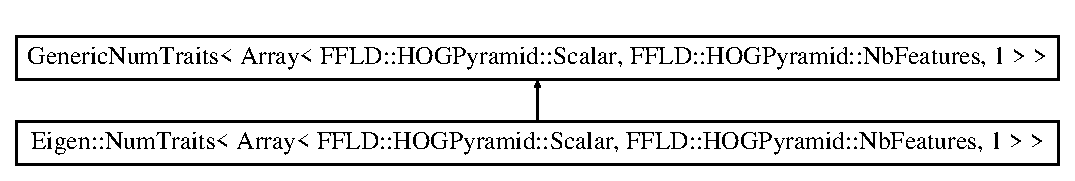
\includegraphics[height=1.978799cm]{struct_eigen_1_1_num_traits_3_01_array_3_01_f_f_l_d_1_1_h_o_g_pyramid_1_1_scalar_00_01_f_f_l_d_179908bda57298c5a601e3a022e5c08f1}
\end{center}
\end{figure}
\subsection*{Static Public Member Functions}
\begin{DoxyCompactItemize}
\item 
\hypertarget{struct_eigen_1_1_num_traits_3_01_array_3_01_f_f_l_d_1_1_h_o_g_pyramid_1_1_scalar_00_01_f_f_l_d_179908bda57298c5a601e3a022e5c08f1_af17f381194aecb89e1c136d2ee408d64}{static \hyperlink{class_f_f_l_d_1_1_h_o_g_pyramid_af17c08ed86557e0a0aecb4814daf87c3}{F\-F\-L\-D\-::\-H\-O\-G\-Pyramid\-::\-Scalar} {\bfseries dummy\-\_\-precision} ()}\label{struct_eigen_1_1_num_traits_3_01_array_3_01_f_f_l_d_1_1_h_o_g_pyramid_1_1_scalar_00_01_f_f_l_d_179908bda57298c5a601e3a022e5c08f1_af17f381194aecb89e1c136d2ee408d64}

\end{DoxyCompactItemize}


The documentation for this struct was generated from the following file\-:\begin{DoxyCompactItemize}
\item 
H\-O\-G\-Pyramid.\-h\end{DoxyCompactItemize}

\hypertarget{struct_eigen_1_1_num_traits_3_01_array_3_01_f_f_l_d_1_1_patchwork_1_1_scalar_00_01_f_f_l_d_1_1_hcd1426a04cfaf6bc4157095debbb74d7}{\section{Eigen\-:\-:Num\-Traits$<$ Array$<$ F\-F\-L\-D\-:\-:Patchwork\-:\-:Scalar, F\-F\-L\-D\-:\-:H\-O\-G\-Pyramid\-:\-:Nb\-Features, 1 $>$ $>$ Struct Template Reference}
\label{struct_eigen_1_1_num_traits_3_01_array_3_01_f_f_l_d_1_1_patchwork_1_1_scalar_00_01_f_f_l_d_1_1_hcd1426a04cfaf6bc4157095debbb74d7}\index{Eigen\-::\-Num\-Traits$<$ Array$<$ F\-F\-L\-D\-::\-Patchwork\-::\-Scalar, F\-F\-L\-D\-::\-H\-O\-G\-Pyramid\-::\-Nb\-Features, 1 $>$ $>$@{Eigen\-::\-Num\-Traits$<$ Array$<$ F\-F\-L\-D\-::\-Patchwork\-::\-Scalar, F\-F\-L\-D\-::\-H\-O\-G\-Pyramid\-::\-Nb\-Features, 1 $>$ $>$}}
}
Inheritance diagram for Eigen\-:\-:Num\-Traits$<$ Array$<$ F\-F\-L\-D\-:\-:Patchwork\-:\-:Scalar, F\-F\-L\-D\-:\-:H\-O\-G\-Pyramid\-:\-:Nb\-Features, 1 $>$ $>$\-:\begin{figure}[H]
\begin{center}
\leavevmode
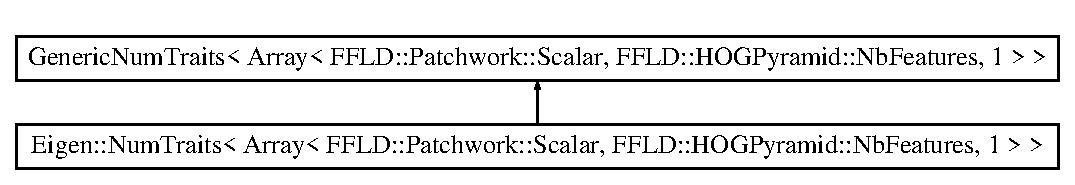
\includegraphics[height=2.000000cm]{struct_eigen_1_1_num_traits_3_01_array_3_01_f_f_l_d_1_1_patchwork_1_1_scalar_00_01_f_f_l_d_1_1_hcd1426a04cfaf6bc4157095debbb74d7}
\end{center}
\end{figure}
\subsection*{Static Public Member Functions}
\begin{DoxyCompactItemize}
\item 
\hypertarget{struct_eigen_1_1_num_traits_3_01_array_3_01_f_f_l_d_1_1_patchwork_1_1_scalar_00_01_f_f_l_d_1_1_hcd1426a04cfaf6bc4157095debbb74d7_a9a62e0bc4289708159eb797b385a1174}{static \hyperlink{class_f_f_l_d_1_1_h_o_g_pyramid_af17c08ed86557e0a0aecb4814daf87c3}{F\-F\-L\-D\-::\-H\-O\-G\-Pyramid\-::\-Scalar} {\bfseries dummy\-\_\-precision} ()}\label{struct_eigen_1_1_num_traits_3_01_array_3_01_f_f_l_d_1_1_patchwork_1_1_scalar_00_01_f_f_l_d_1_1_hcd1426a04cfaf6bc4157095debbb74d7_a9a62e0bc4289708159eb797b385a1174}

\end{DoxyCompactItemize}


The documentation for this struct was generated from the following file\-:\begin{DoxyCompactItemize}
\item 
Patchwork.\-h\end{DoxyCompactItemize}

\hypertarget{class_f_f_l_d_1_1_object}{\section{F\-F\-L\-D\-:\-:Object Class Reference}
\label{class_f_f_l_d_1_1_object}\index{F\-F\-L\-D\-::\-Object@{F\-F\-L\-D\-::\-Object}}
}


{\ttfamily \#include $<$Object.\-h$>$}

\subsection*{Public Types}
\begin{DoxyCompactItemize}
\item 
enum \hyperlink{class_f_f_l_d_1_1_object_a4db6ef6debc5011ab6da14f251fd3a32}{Name} \{ \\*
{\bfseries A\-E\-R\-O\-P\-L\-A\-N\-E}, 
{\bfseries B\-I\-C\-Y\-C\-L\-E}, 
{\bfseries B\-I\-R\-D}, 
{\bfseries B\-O\-A\-T}, 
\\*
{\bfseries B\-O\-T\-T\-L\-E}, 
{\bfseries B\-U\-S}, 
{\bfseries C\-A\-R}, 
{\bfseries C\-A\-T}, 
\\*
{\bfseries C\-H\-A\-I\-R}, 
{\bfseries C\-O\-W}, 
{\bfseries D\-I\-N\-I\-N\-G\-T\-A\-B\-L\-E}, 
{\bfseries D\-O\-G}, 
\\*
{\bfseries H\-O\-R\-S\-E}, 
{\bfseries M\-O\-T\-O\-R\-B\-I\-K\-E}, 
{\bfseries P\-E\-R\-S\-O\-N}, 
{\bfseries P\-O\-T\-T\-E\-D\-P\-L\-A\-N\-T}, 
\\*
{\bfseries S\-H\-E\-E\-P}, 
{\bfseries S\-O\-F\-A}, 
{\bfseries T\-R\-A\-I\-N}, 
{\bfseries T\-V\-M\-O\-N\-I\-T\-O\-R}, 
\\*
{\bfseries U\-N\-K\-N\-O\-W\-N}
 \}
\begin{DoxyCompactList}\small\item\em The possible object labels. \end{DoxyCompactList}\item 
enum \hyperlink{class_f_f_l_d_1_1_object_a922b08e7fb8e69b9092b01eee82cd7ec}{Pose} \{ \\*
{\bfseries F\-R\-O\-N\-T\-A\-L}, 
{\bfseries L\-E\-F\-T}, 
{\bfseries R\-E\-A\-R}, 
{\bfseries R\-I\-G\-H\-T}, 
\\*
{\bfseries U\-N\-S\-P\-E\-C\-I\-F\-I\-E\-D}
 \}
\begin{DoxyCompactList}\small\item\em The possible object views. \end{DoxyCompactList}\end{DoxyCompactItemize}
\subsection*{Public Member Functions}
\begin{DoxyCompactItemize}
\item 
\hyperlink{class_f_f_l_d_1_1_object_a40860402e64d8008fb42329df7097cdb}{Object} ()
\item 
\hyperlink{class_f_f_l_d_1_1_object_a1078bdbbda7eec829d8f11717ea65970}{Object} (\hyperlink{class_f_f_l_d_1_1_object_a4db6ef6debc5011ab6da14f251fd3a32}{Name} \hyperlink{class_f_f_l_d_1_1_object_aa8b7117e7bec7bac930b7577a5dc528a}{name}, \hyperlink{class_f_f_l_d_1_1_object_a922b08e7fb8e69b9092b01eee82cd7ec}{Pose} \hyperlink{class_f_f_l_d_1_1_object_a370d8f00e19a2fedbf29c0f99804f1a1}{pose}, bool \hyperlink{class_f_f_l_d_1_1_object_aeb5fb9d9d6b975438b441d31230261e3}{truncated}, bool \hyperlink{class_f_f_l_d_1_1_object_a7316217057e6c76b57cd37b570d8c24f}{difficult}, \hyperlink{class_f_f_l_d_1_1_rectangle}{Rectangle} \hyperlink{class_f_f_l_d_1_1_object_a2dd49cdfad84ccaf0ef821438b5e8aa9}{bndbox})
\item 
\hypertarget{class_f_f_l_d_1_1_object_aa8b7117e7bec7bac930b7577a5dc528a}{\hyperlink{class_f_f_l_d_1_1_object_a4db6ef6debc5011ab6da14f251fd3a32}{Name} \hyperlink{class_f_f_l_d_1_1_object_aa8b7117e7bec7bac930b7577a5dc528a}{name} () const }\label{class_f_f_l_d_1_1_object_aa8b7117e7bec7bac930b7577a5dc528a}

\begin{DoxyCompactList}\small\item\em Returns the name (label) of the object. \end{DoxyCompactList}\item 
\hypertarget{class_f_f_l_d_1_1_object_a86018800797a71678aab85b62d865b1b}{void \hyperlink{class_f_f_l_d_1_1_object_a86018800797a71678aab85b62d865b1b}{set\-Name} (\hyperlink{class_f_f_l_d_1_1_object_a4db6ef6debc5011ab6da14f251fd3a32}{Name} \hyperlink{class_f_f_l_d_1_1_object_aa8b7117e7bec7bac930b7577a5dc528a}{name})}\label{class_f_f_l_d_1_1_object_a86018800797a71678aab85b62d865b1b}

\begin{DoxyCompactList}\small\item\em Sets the name (label) of the object. \end{DoxyCompactList}\item 
\hypertarget{class_f_f_l_d_1_1_object_a370d8f00e19a2fedbf29c0f99804f1a1}{\hyperlink{class_f_f_l_d_1_1_object_a922b08e7fb8e69b9092b01eee82cd7ec}{Pose} \hyperlink{class_f_f_l_d_1_1_object_a370d8f00e19a2fedbf29c0f99804f1a1}{pose} () const }\label{class_f_f_l_d_1_1_object_a370d8f00e19a2fedbf29c0f99804f1a1}

\begin{DoxyCompactList}\small\item\em Returns the pose (view) of the object. \end{DoxyCompactList}\item 
\hypertarget{class_f_f_l_d_1_1_object_a8bdb30bfb3d86ce087705914a6f08ca1}{void \hyperlink{class_f_f_l_d_1_1_object_a8bdb30bfb3d86ce087705914a6f08ca1}{set\-Pose} (\hyperlink{class_f_f_l_d_1_1_object_a922b08e7fb8e69b9092b01eee82cd7ec}{Pose} \hyperlink{class_f_f_l_d_1_1_object_a370d8f00e19a2fedbf29c0f99804f1a1}{pose})}\label{class_f_f_l_d_1_1_object_a8bdb30bfb3d86ce087705914a6f08ca1}

\begin{DoxyCompactList}\small\item\em Sets the pose (view) of the object. \end{DoxyCompactList}\item 
\hypertarget{class_f_f_l_d_1_1_object_aeb5fb9d9d6b975438b441d31230261e3}{bool \hyperlink{class_f_f_l_d_1_1_object_aeb5fb9d9d6b975438b441d31230261e3}{truncated} () const }\label{class_f_f_l_d_1_1_object_aeb5fb9d9d6b975438b441d31230261e3}

\begin{DoxyCompactList}\small\item\em Returns whether the object is annotated as being truncated. \end{DoxyCompactList}\item 
\hypertarget{class_f_f_l_d_1_1_object_ad2edf2a24c537ce7731e9425a049d224}{void \hyperlink{class_f_f_l_d_1_1_object_ad2edf2a24c537ce7731e9425a049d224}{set\-Truncated} (bool \hyperlink{class_f_f_l_d_1_1_object_aeb5fb9d9d6b975438b441d31230261e3}{truncated})}\label{class_f_f_l_d_1_1_object_ad2edf2a24c537ce7731e9425a049d224}

\begin{DoxyCompactList}\small\item\em Annotates the object as being truncated. \end{DoxyCompactList}\item 
\hypertarget{class_f_f_l_d_1_1_object_a7316217057e6c76b57cd37b570d8c24f}{bool \hyperlink{class_f_f_l_d_1_1_object_a7316217057e6c76b57cd37b570d8c24f}{difficult} () const }\label{class_f_f_l_d_1_1_object_a7316217057e6c76b57cd37b570d8c24f}

\begin{DoxyCompactList}\small\item\em Returns whether the object is annotated as being difficult. \end{DoxyCompactList}\item 
\hypertarget{class_f_f_l_d_1_1_object_a9d090f14838946494fad4e12480396c0}{void \hyperlink{class_f_f_l_d_1_1_object_a9d090f14838946494fad4e12480396c0}{set\-Difficult} (bool \hyperlink{class_f_f_l_d_1_1_object_a7316217057e6c76b57cd37b570d8c24f}{difficult})}\label{class_f_f_l_d_1_1_object_a9d090f14838946494fad4e12480396c0}

\begin{DoxyCompactList}\small\item\em Annotates the object as being difficult. \end{DoxyCompactList}\item 
\hypertarget{class_f_f_l_d_1_1_object_a2dd49cdfad84ccaf0ef821438b5e8aa9}{\hyperlink{class_f_f_l_d_1_1_rectangle}{Rectangle} \hyperlink{class_f_f_l_d_1_1_object_a2dd49cdfad84ccaf0ef821438b5e8aa9}{bndbox} () const }\label{class_f_f_l_d_1_1_object_a2dd49cdfad84ccaf0ef821438b5e8aa9}

\begin{DoxyCompactList}\small\item\em Returns the bounding box of the object. \end{DoxyCompactList}\item 
\hypertarget{class_f_f_l_d_1_1_object_a2797d2e00d013b11ab1e82e6903fba6e}{void \hyperlink{class_f_f_l_d_1_1_object_a2797d2e00d013b11ab1e82e6903fba6e}{set\-Bndbox} (\hyperlink{class_f_f_l_d_1_1_rectangle}{Rectangle} \hyperlink{class_f_f_l_d_1_1_object_a2dd49cdfad84ccaf0ef821438b5e8aa9}{bndbox})}\label{class_f_f_l_d_1_1_object_a2797d2e00d013b11ab1e82e6903fba6e}

\begin{DoxyCompactList}\small\item\em Sets the bounding box of the object. \end{DoxyCompactList}\item 
bool \hyperlink{class_f_f_l_d_1_1_object_aba86e2335f3c2b2db9be38c188bf04e4}{empty} () const 
\end{DoxyCompactItemize}


\subsection{Detailed Description}
The \hyperlink{class_f_f_l_d_1_1_object}{Object} class represents an object in a \hyperlink{class_f_f_l_d_1_1_scene}{Scene}. It stores all the information present inbetween $<$object$>$ tags in a Pascal V\-O\-C 2007 .xml annotation file, although the bounding box is represented slightly differently (top left coordinates of (0, 0) instead of (1, 1)). 

\subsection{Constructor \& Destructor Documentation}
\hypertarget{class_f_f_l_d_1_1_object_a40860402e64d8008fb42329df7097cdb}{\index{F\-F\-L\-D\-::\-Object@{F\-F\-L\-D\-::\-Object}!Object@{Object}}
\index{Object@{Object}!FFLD::Object@{F\-F\-L\-D\-::\-Object}}
\subsubsection[{Object}]{\setlength{\rightskip}{0pt plus 5cm}Object\-::\-Object (
\begin{DoxyParamCaption}
{}
\end{DoxyParamCaption}
)}}\label{class_f_f_l_d_1_1_object_a40860402e64d8008fb42329df7097cdb}
Constructs an empty object. An empty object has name 'unknown', pose 'unspecified', and all other parameters set to their default values. \hypertarget{class_f_f_l_d_1_1_object_a1078bdbbda7eec829d8f11717ea65970}{\index{F\-F\-L\-D\-::\-Object@{F\-F\-L\-D\-::\-Object}!Object@{Object}}
\index{Object@{Object}!FFLD::Object@{F\-F\-L\-D\-::\-Object}}
\subsubsection[{Object}]{\setlength{\rightskip}{0pt plus 5cm}Object\-::\-Object (
\begin{DoxyParamCaption}
\item[{{\bf Name}}]{name, }
\item[{{\bf Pose}}]{pose, }
\item[{bool}]{truncated, }
\item[{bool}]{difficult, }
\item[{{\bf Rectangle}}]{bndbox}
\end{DoxyParamCaption}
)}}\label{class_f_f_l_d_1_1_object_a1078bdbbda7eec829d8f11717ea65970}
Constructs an object from a name, a pose, annotation flags and a bounding box. 
\begin{DoxyParams}[1]{Parameters}
\mbox{\tt in}  & {\em name} & Label of the object. \\
\hline
\mbox{\tt in}  & {\em pose} & View of the object. \\
\hline
\mbox{\tt in}  & {\em truncated} & Whether the object is annotated as being truncated. \\
\hline
\mbox{\tt in}  & {\em difficult} & Whether the object is annotated as being difficult. \\
\hline
\mbox{\tt in}  & {\em bndbox} & Bounding box of the object. \\
\hline
\end{DoxyParams}


\subsection{Member Function Documentation}
\hypertarget{class_f_f_l_d_1_1_object_aba86e2335f3c2b2db9be38c188bf04e4}{\index{F\-F\-L\-D\-::\-Object@{F\-F\-L\-D\-::\-Object}!empty@{empty}}
\index{empty@{empty}!FFLD::Object@{F\-F\-L\-D\-::\-Object}}
\subsubsection[{empty}]{\setlength{\rightskip}{0pt plus 5cm}bool Object\-::empty (
\begin{DoxyParamCaption}
{}
\end{DoxyParamCaption}
) const}}\label{class_f_f_l_d_1_1_object_aba86e2335f3c2b2db9be38c188bf04e4}
Returns whether the object is empty. An empty object has name 'unknown', pose 'unspecified', and all other parameters set to their default values. 

The documentation for this class was generated from the following files\-:\begin{DoxyCompactItemize}
\item 
Object.\-h\item 
Object.\-cpp\end{DoxyCompactItemize}

\hypertarget{class_f_f_l_d_1_1_patchwork}{\section{F\-F\-L\-D\-:\-:Patchwork Class Reference}
\label{class_f_f_l_d_1_1_patchwork}\index{F\-F\-L\-D\-::\-Patchwork@{F\-F\-L\-D\-::\-Patchwork}}
}


The \hyperlink{class_f_f_l_d_1_1_patchwork}{Patchwork} class computes full convolutions much faster than the \hyperlink{class_f_f_l_d_1_1_h_o_g_pyramid}{H\-O\-G\-Pyramid} class.  




{\ttfamily \#include $<$Patchwork.\-h$>$}

\subsection*{Public Types}
\begin{DoxyCompactItemize}
\item 
\hypertarget{class_f_f_l_d_1_1_patchwork_aa1945335907399a846b7595f9215a2a3}{typedef std\-::complex\\*
$<$ \hyperlink{class_f_f_l_d_1_1_h_o_g_pyramid_af17c08ed86557e0a0aecb4814daf87c3}{H\-O\-G\-Pyramid\-::\-Scalar} $>$ \hyperlink{class_f_f_l_d_1_1_patchwork_aa1945335907399a846b7595f9215a2a3}{Scalar}}\label{class_f_f_l_d_1_1_patchwork_aa1945335907399a846b7595f9215a2a3}

\begin{DoxyCompactList}\small\item\em Type of a scalar value. \end{DoxyCompactList}\item 
\hypertarget{class_f_f_l_d_1_1_patchwork_ad50017d26020d6cc25061f62765eedf7}{typedef Eigen\-::\-Matrix$<$ \hyperlink{class_f_f_l_d_1_1_patchwork_aa1945335907399a846b7595f9215a2a3}{Scalar}, \\*
Eigen\-::\-Dynamic, Eigen\-::\-Dynamic, \\*
Eigen\-::\-Row\-Major $>$ \hyperlink{class_f_f_l_d_1_1_patchwork_ad50017d26020d6cc25061f62765eedf7}{Matrix}}\label{class_f_f_l_d_1_1_patchwork_ad50017d26020d6cc25061f62765eedf7}

\begin{DoxyCompactList}\small\item\em Type of a matrix. \end{DoxyCompactList}\item 
\hypertarget{class_f_f_l_d_1_1_patchwork_a2a631726c87e622e21c374c340b673cf}{typedef Eigen\-::\-Array$<$ \hyperlink{class_f_f_l_d_1_1_patchwork_aa1945335907399a846b7595f9215a2a3}{Scalar}, \\*
\hyperlink{class_f_f_l_d_1_1_h_o_g_pyramid_a418ebc8cf8781a3874f50b5eac482c68}{H\-O\-G\-Pyramid\-::\-Nb\-Features}, 1 $>$ \hyperlink{class_f_f_l_d_1_1_patchwork_a2a631726c87e622e21c374c340b673cf}{Cell}}\label{class_f_f_l_d_1_1_patchwork_a2a631726c87e622e21c374c340b673cf}

\begin{DoxyCompactList}\small\item\em Type of a patchwork plane cell (fixed-\/size complex vector of size Nb\-Features). \end{DoxyCompactList}\item 
\hypertarget{class_f_f_l_d_1_1_patchwork_a119551af7ed0303c3d6a0396ff4d3d39}{typedef Eigen\-::\-Matrix$<$ \hyperlink{class_f_f_l_d_1_1_patchwork_a2a631726c87e622e21c374c340b673cf}{Cell}, \\*
Eigen\-::\-Dynamic, Eigen\-::\-Dynamic, \\*
Eigen\-::\-Row\-Major $>$ \hyperlink{class_f_f_l_d_1_1_patchwork_a119551af7ed0303c3d6a0396ff4d3d39}{Plane}}\label{class_f_f_l_d_1_1_patchwork_a119551af7ed0303c3d6a0396ff4d3d39}

\begin{DoxyCompactList}\small\item\em Type of a patchwork plane (matrix of cells). \end{DoxyCompactList}\item 
\hypertarget{class_f_f_l_d_1_1_patchwork_aa342f3a41430505b16a53c3e2683c497}{typedef std\-::pair$<$ \hyperlink{class_f_f_l_d_1_1_patchwork_a119551af7ed0303c3d6a0396ff4d3d39}{Plane}, \\*
std\-::pair$<$ int, int $>$ $>$ \hyperlink{class_f_f_l_d_1_1_patchwork_aa342f3a41430505b16a53c3e2683c497}{Filter}}\label{class_f_f_l_d_1_1_patchwork_aa342f3a41430505b16a53c3e2683c497}

\begin{DoxyCompactList}\small\item\em Type of a patchwork filter (plane + original filter size). \end{DoxyCompactList}\end{DoxyCompactItemize}
\subsection*{Public Member Functions}
\begin{DoxyCompactItemize}
\item 
\hypertarget{class_f_f_l_d_1_1_patchwork_a57c40d2ceddfb9dd64efb9b2bb5d9a9e}{\hyperlink{class_f_f_l_d_1_1_patchwork_a57c40d2ceddfb9dd64efb9b2bb5d9a9e}{Patchwork} ()}\label{class_f_f_l_d_1_1_patchwork_a57c40d2ceddfb9dd64efb9b2bb5d9a9e}

\begin{DoxyCompactList}\small\item\em Constructs an empty patchwork. An empty patchwork has no plane. \end{DoxyCompactList}\item 
\hyperlink{class_f_f_l_d_1_1_patchwork_aa38d8158bbfff82f625d7ddae0b5cd58}{Patchwork} (const \hyperlink{class_f_f_l_d_1_1_h_o_g_pyramid}{H\-O\-G\-Pyramid} \&pyramid)
\item 
\hypertarget{class_f_f_l_d_1_1_patchwork_ae16a7a8143f5a8b05cf9d54ae2d4b262}{int \hyperlink{class_f_f_l_d_1_1_patchwork_ae16a7a8143f5a8b05cf9d54ae2d4b262}{padx} () const }\label{class_f_f_l_d_1_1_patchwork_ae16a7a8143f5a8b05cf9d54ae2d4b262}

\begin{DoxyCompactList}\small\item\em Returns the amount of horizontal zero padding (in cells). \end{DoxyCompactList}\item 
\hypertarget{class_f_f_l_d_1_1_patchwork_ab9275f8b38a747ab59fc2c54f89d8b62}{int \hyperlink{class_f_f_l_d_1_1_patchwork_ab9275f8b38a747ab59fc2c54f89d8b62}{pady} () const }\label{class_f_f_l_d_1_1_patchwork_ab9275f8b38a747ab59fc2c54f89d8b62}

\begin{DoxyCompactList}\small\item\em Returns the amount of vertical zero padding (in cells). \end{DoxyCompactList}\item 
\hypertarget{class_f_f_l_d_1_1_patchwork_a37da8d780e23b79eeeea570a0a888da1}{int \hyperlink{class_f_f_l_d_1_1_patchwork_a37da8d780e23b79eeeea570a0a888da1}{interval} () const }\label{class_f_f_l_d_1_1_patchwork_a37da8d780e23b79eeeea570a0a888da1}

\begin{DoxyCompactList}\small\item\em Returns the number of levels per octave in the pyramid. \end{DoxyCompactList}\item 
\hypertarget{class_f_f_l_d_1_1_patchwork_a33d7a3b3e96b48a05ba23ca558d09f33}{bool \hyperlink{class_f_f_l_d_1_1_patchwork_a33d7a3b3e96b48a05ba23ca558d09f33}{empty} () const }\label{class_f_f_l_d_1_1_patchwork_a33d7a3b3e96b48a05ba23ca558d09f33}

\begin{DoxyCompactList}\small\item\em Returns whether the patchwork is empty. An empty patchwork has no plane. \end{DoxyCompactList}\item 
void \hyperlink{class_f_f_l_d_1_1_patchwork_a52eadb033fc06793960507cd9c6e15cb}{convolve} (const std\-::vector$<$ \hyperlink{class_f_f_l_d_1_1_patchwork_aa342f3a41430505b16a53c3e2683c497}{Filter} $>$ \&filters, std\-::vector$<$ std\-::vector$<$ \hyperlink{class_f_f_l_d_1_1_h_o_g_pyramid_a2618b4bd5d17f05cdc108189ed5abe3a}{H\-O\-G\-Pyramid\-::\-Matrix} $>$ $>$ \&convolutions) const 
\end{DoxyCompactItemize}
\subsection*{Static Public Member Functions}
\begin{DoxyCompactItemize}
\item 
static bool \hyperlink{class_f_f_l_d_1_1_patchwork_ac4aecde334ba92e8322962c7a1ae3dba}{Init} (int max\-Rows, int max\-Cols)
\item 
\hypertarget{class_f_f_l_d_1_1_patchwork_af8839b72f5a03b58d755b63237f7b3ab}{static int \hyperlink{class_f_f_l_d_1_1_patchwork_af8839b72f5a03b58d755b63237f7b3ab}{Max\-Rows} ()}\label{class_f_f_l_d_1_1_patchwork_af8839b72f5a03b58d755b63237f7b3ab}

\begin{DoxyCompactList}\small\item\em Returns the current maximum number of rows of a pyramid level (including padding). \end{DoxyCompactList}\item 
\hypertarget{class_f_f_l_d_1_1_patchwork_a46e9cff798e51e0c602a8a9cc382b314}{static int \hyperlink{class_f_f_l_d_1_1_patchwork_a46e9cff798e51e0c602a8a9cc382b314}{Max\-Cols} ()}\label{class_f_f_l_d_1_1_patchwork_a46e9cff798e51e0c602a8a9cc382b314}

\begin{DoxyCompactList}\small\item\em Returns the current maximum number of columns of a pyramid level (including padding). \end{DoxyCompactList}\item 
static void \hyperlink{class_f_f_l_d_1_1_patchwork_ad920b3c00b4b2baa4fb08433ee0a08e1}{Transform\-Filter} (const \hyperlink{class_f_f_l_d_1_1_h_o_g_pyramid_a1cd36670adf29538f44dfa434695ec34}{H\-O\-G\-Pyramid\-::\-Level} \&filter, \hyperlink{class_f_f_l_d_1_1_patchwork_aa342f3a41430505b16a53c3e2683c497}{Filter} \&result)
\end{DoxyCompactItemize}


\subsection{Detailed Description}
The \hyperlink{class_f_f_l_d_1_1_patchwork}{Patchwork} class computes full convolutions much faster than the \hyperlink{class_f_f_l_d_1_1_h_o_g_pyramid}{H\-O\-G\-Pyramid} class. 

\subsection{Constructor \& Destructor Documentation}
\hypertarget{class_f_f_l_d_1_1_patchwork_aa38d8158bbfff82f625d7ddae0b5cd58}{\index{F\-F\-L\-D\-::\-Patchwork@{F\-F\-L\-D\-::\-Patchwork}!Patchwork@{Patchwork}}
\index{Patchwork@{Patchwork}!FFLD::Patchwork@{F\-F\-L\-D\-::\-Patchwork}}
\subsubsection[{Patchwork}]{\setlength{\rightskip}{0pt plus 5cm}Patchwork\-::\-Patchwork (
\begin{DoxyParamCaption}
\item[{const {\bf H\-O\-G\-Pyramid} \&}]{pyramid}
\end{DoxyParamCaption}
)}}\label{class_f_f_l_d_1_1_patchwork_aa38d8158bbfff82f625d7ddae0b5cd58}
Constructs a patchwork from a pyramid. 
\begin{DoxyParams}[1]{Parameters}
\mbox{\tt in}  & {\em pyramid} & The pyramid of features. \\
\hline
\end{DoxyParams}
\begin{DoxyNote}{Note}
If the pyramid is larger than the last max\-Rows and max\-Cols passed to the Init method the \hyperlink{class_f_f_l_d_1_1_patchwork}{Patchwork} will be empty. 

Assumes that the features of the pyramid levels are zero in the padded regions but for the last feature, which is assumed to be one. 
\end{DoxyNote}


\subsection{Member Function Documentation}
\hypertarget{class_f_f_l_d_1_1_patchwork_a52eadb033fc06793960507cd9c6e15cb}{\index{F\-F\-L\-D\-::\-Patchwork@{F\-F\-L\-D\-::\-Patchwork}!convolve@{convolve}}
\index{convolve@{convolve}!FFLD::Patchwork@{F\-F\-L\-D\-::\-Patchwork}}
\subsubsection[{convolve}]{\setlength{\rightskip}{0pt plus 5cm}void Patchwork\-::convolve (
\begin{DoxyParamCaption}
\item[{const std\-::vector$<$ {\bf Filter} $>$ \&}]{filters, }
\item[{std\-::vector$<$ std\-::vector$<$ {\bf H\-O\-G\-Pyramid\-::\-Matrix} $>$ $>$ \&}]{convolutions}
\end{DoxyParamCaption}
) const}}\label{class_f_f_l_d_1_1_patchwork_a52eadb033fc06793960507cd9c6e15cb}
Returns the convolutions of the patchwork with filters (useful to compute the S\-V\-M margins). 
\begin{DoxyParams}[1]{Parameters}
\mbox{\tt in}  & {\em filters} & The filters. \\
\hline
\mbox{\tt out}  & {\em convolutions} & The convolutions (filters x levels). \\
\hline
\end{DoxyParams}
\hypertarget{class_f_f_l_d_1_1_patchwork_ac4aecde334ba92e8322962c7a1ae3dba}{\index{F\-F\-L\-D\-::\-Patchwork@{F\-F\-L\-D\-::\-Patchwork}!Init@{Init}}
\index{Init@{Init}!FFLD::Patchwork@{F\-F\-L\-D\-::\-Patchwork}}
\subsubsection[{Init}]{\setlength{\rightskip}{0pt plus 5cm}bool Patchwork\-::\-Init (
\begin{DoxyParamCaption}
\item[{int}]{max\-Rows, }
\item[{int}]{max\-Cols}
\end{DoxyParamCaption}
)\hspace{0.3cm}{\ttfamily [static]}}}\label{class_f_f_l_d_1_1_patchwork_ac4aecde334ba92e8322962c7a1ae3dba}
Initializes the F\-F\-T\-W library. 
\begin{DoxyParams}[1]{Parameters}
\mbox{\tt in}  & {\em max\-Rows} & Maximum number of rows of a pyramid level (including padding). \\
\hline
\mbox{\tt in}  & {\em max\-Cols} & Maximum number of columns of a pyramid level (including padding). \\
\hline
\end{DoxyParams}
\begin{DoxyReturn}{Returns}
Whether the initialization was successful. 
\end{DoxyReturn}
\begin{DoxyNote}{Note}
Must be called before any other method (including constructors). 
\end{DoxyNote}
\hypertarget{class_f_f_l_d_1_1_patchwork_ad920b3c00b4b2baa4fb08433ee0a08e1}{\index{F\-F\-L\-D\-::\-Patchwork@{F\-F\-L\-D\-::\-Patchwork}!Transform\-Filter@{Transform\-Filter}}
\index{Transform\-Filter@{Transform\-Filter}!FFLD::Patchwork@{F\-F\-L\-D\-::\-Patchwork}}
\subsubsection[{Transform\-Filter}]{\setlength{\rightskip}{0pt plus 5cm}void Patchwork\-::\-Transform\-Filter (
\begin{DoxyParamCaption}
\item[{const {\bf H\-O\-G\-Pyramid\-::\-Level} \&}]{filter, }
\item[{{\bf Filter} \&}]{result}
\end{DoxyParamCaption}
)\hspace{0.3cm}{\ttfamily [static]}}}\label{class_f_f_l_d_1_1_patchwork_ad920b3c00b4b2baa4fb08433ee0a08e1}
Returns a transformed version of a filter to be used by the {\ttfamily convolve} method. 
\begin{DoxyParams}[1]{Parameters}
\mbox{\tt in}  & {\em filter} & Filter to transform. \\
\hline
\mbox{\tt out}  & {\em result} & Transformed filter. \\
\hline
\end{DoxyParams}
\begin{DoxyNote}{Note}
If Init was not already called or if the filter is larger than the last max\-Rows and max\-Cols passed to the Init method the result will be empty. 
\end{DoxyNote}


The documentation for this class was generated from the following files\-:\begin{DoxyCompactItemize}
\item 
Patchwork.\-h\item 
Patchwork.\-cpp\end{DoxyCompactItemize}

\hypertarget{struct_f_f_l_d_1_1detail_1_1_position_comparator}{\section{F\-F\-L\-D\-:\-:detail\-:\-:Position\-Comparator Struct Reference}
\label{struct_f_f_l_d_1_1detail_1_1_position_comparator}\index{F\-F\-L\-D\-::detail\-::\-Position\-Comparator@{F\-F\-L\-D\-::detail\-::\-Position\-Comparator}}
}
\subsection*{Public Member Functions}
\begin{DoxyCompactItemize}
\item 
\hypertarget{struct_f_f_l_d_1_1detail_1_1_position_comparator_a18bec662e49d613889bf64fbb88c3b87}{bool {\bfseries operator()} (const \hyperlink{class_f_f_l_d_1_1_rectangle}{Rectangle} \&a, const \hyperlink{class_f_f_l_d_1_1_rectangle}{Rectangle} \&b) const }\label{struct_f_f_l_d_1_1detail_1_1_position_comparator_a18bec662e49d613889bf64fbb88c3b87}

\end{DoxyCompactItemize}


The documentation for this struct was generated from the following file\-:\begin{DoxyCompactItemize}
\item 
/\-Users/raphaeldendooven/\-Documents/school/2013-\/2014\-\_\-\-Thesis\-\_\-\-Master/\-Programs/\-Hand\-Detection/Patchwork.\-cpp\end{DoxyCompactItemize}

\hypertarget{class_f_f_l_d_1_1_rectangle}{\section{F\-F\-L\-D\-:\-:Rectangle Class Reference}
\label{class_f_f_l_d_1_1_rectangle}\index{F\-F\-L\-D\-::\-Rectangle@{F\-F\-L\-D\-::\-Rectangle}}
}


{\ttfamily \#include $<$Rectangle.\-h$>$}

Inheritance diagram for F\-F\-L\-D\-:\-:Rectangle\-:\begin{figure}[H]
\begin{center}
\leavevmode
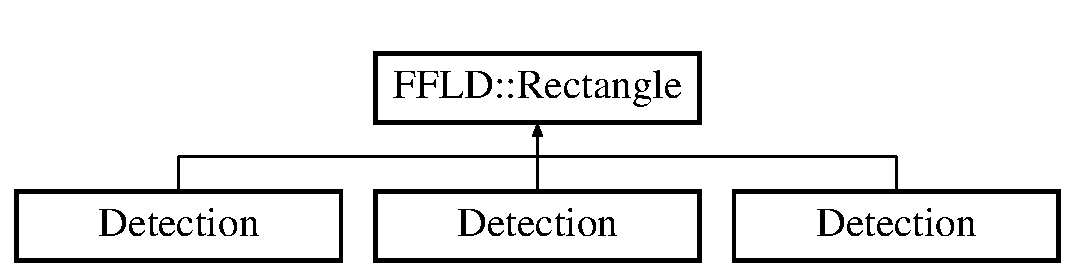
\includegraphics[height=2.000000cm]{class_f_f_l_d_1_1_rectangle}
\end{center}
\end{figure}
\subsection*{Public Member Functions}
\begin{DoxyCompactItemize}
\item 
\hypertarget{class_f_f_l_d_1_1_rectangle_a8a933e0ebd9e80ce91e61ffe87fd577e}{\hyperlink{class_f_f_l_d_1_1_rectangle_a8a933e0ebd9e80ce91e61ffe87fd577e}{Rectangle} ()}\label{class_f_f_l_d_1_1_rectangle_a8a933e0ebd9e80ce91e61ffe87fd577e}

\begin{DoxyCompactList}\small\item\em Constructs an empty rectangle. An empty rectangle has no area. \end{DoxyCompactList}\item 
\hypertarget{class_f_f_l_d_1_1_rectangle_a6075b7065a6cfb2e4007030d07f0d7be}{\hyperlink{class_f_f_l_d_1_1_rectangle_a6075b7065a6cfb2e4007030d07f0d7be}{Rectangle} (int \hyperlink{class_f_f_l_d_1_1_rectangle_af62553af29f32815e5055f67b96f5603}{width}, int \hyperlink{class_f_f_l_d_1_1_rectangle_a51fcde43e3b8803b7fcf3bba60167894}{height})}\label{class_f_f_l_d_1_1_rectangle_a6075b7065a6cfb2e4007030d07f0d7be}

\begin{DoxyCompactList}\small\item\em Constructs a rectangle with the given {\ttfamily width} and {\ttfamily height}. \end{DoxyCompactList}\item 
\hypertarget{class_f_f_l_d_1_1_rectangle_a6fd48c1264965fd841b2d35b7736a352}{\hyperlink{class_f_f_l_d_1_1_rectangle_a6fd48c1264965fd841b2d35b7736a352}{Rectangle} (int \hyperlink{class_f_f_l_d_1_1_rectangle_aeb9afe5d3ed04bc0158205488260b48b}{x}, int \hyperlink{class_f_f_l_d_1_1_rectangle_a2e8a52081b2efe4f08d4bcabb9ee8cc5}{y}, int \hyperlink{class_f_f_l_d_1_1_rectangle_af62553af29f32815e5055f67b96f5603}{width}, int \hyperlink{class_f_f_l_d_1_1_rectangle_a51fcde43e3b8803b7fcf3bba60167894}{height})}\label{class_f_f_l_d_1_1_rectangle_a6fd48c1264965fd841b2d35b7736a352}

\begin{DoxyCompactList}\small\item\em Constructs a rectangle with coordinates ({\ttfamily x}, {\ttfamily y}) and the given {\ttfamily width} and {\ttfamily height}. \end{DoxyCompactList}\item 
\hypertarget{class_f_f_l_d_1_1_rectangle_aeb9afe5d3ed04bc0158205488260b48b}{int \hyperlink{class_f_f_l_d_1_1_rectangle_aeb9afe5d3ed04bc0158205488260b48b}{x} () const }\label{class_f_f_l_d_1_1_rectangle_aeb9afe5d3ed04bc0158205488260b48b}

\begin{DoxyCompactList}\small\item\em Returns the x-\/coordinate of the rectangle. \end{DoxyCompactList}\item 
\hypertarget{class_f_f_l_d_1_1_rectangle_a852214720fc2e2ce51c255af67180d5f}{void \hyperlink{class_f_f_l_d_1_1_rectangle_a852214720fc2e2ce51c255af67180d5f}{set\-X} (int \hyperlink{class_f_f_l_d_1_1_rectangle_aeb9afe5d3ed04bc0158205488260b48b}{x})}\label{class_f_f_l_d_1_1_rectangle_a852214720fc2e2ce51c255af67180d5f}

\begin{DoxyCompactList}\small\item\em Sets the x coordinate of the rectangle to {\ttfamily x}. \end{DoxyCompactList}\item 
\hypertarget{class_f_f_l_d_1_1_rectangle_a2e8a52081b2efe4f08d4bcabb9ee8cc5}{int \hyperlink{class_f_f_l_d_1_1_rectangle_a2e8a52081b2efe4f08d4bcabb9ee8cc5}{y} () const }\label{class_f_f_l_d_1_1_rectangle_a2e8a52081b2efe4f08d4bcabb9ee8cc5}

\begin{DoxyCompactList}\small\item\em Returns the y-\/coordinate of the rectangle. \end{DoxyCompactList}\item 
\hypertarget{class_f_f_l_d_1_1_rectangle_a64ba58c728d02e731491581bb0e6c857}{void \hyperlink{class_f_f_l_d_1_1_rectangle_a64ba58c728d02e731491581bb0e6c857}{set\-Y} (int \hyperlink{class_f_f_l_d_1_1_rectangle_a2e8a52081b2efe4f08d4bcabb9ee8cc5}{y})}\label{class_f_f_l_d_1_1_rectangle_a64ba58c728d02e731491581bb0e6c857}

\begin{DoxyCompactList}\small\item\em Sets the y coordinate of the rectangle to {\ttfamily y}. \end{DoxyCompactList}\item 
\hypertarget{class_f_f_l_d_1_1_rectangle_af62553af29f32815e5055f67b96f5603}{int \hyperlink{class_f_f_l_d_1_1_rectangle_af62553af29f32815e5055f67b96f5603}{width} () const }\label{class_f_f_l_d_1_1_rectangle_af62553af29f32815e5055f67b96f5603}

\begin{DoxyCompactList}\small\item\em Returns the width of the rectangle. \end{DoxyCompactList}\item 
\hypertarget{class_f_f_l_d_1_1_rectangle_af8a285283f01dad19b6ad355a16da95a}{void \hyperlink{class_f_f_l_d_1_1_rectangle_af8a285283f01dad19b6ad355a16da95a}{set\-Width} (int \hyperlink{class_f_f_l_d_1_1_rectangle_af62553af29f32815e5055f67b96f5603}{width})}\label{class_f_f_l_d_1_1_rectangle_af8a285283f01dad19b6ad355a16da95a}

\begin{DoxyCompactList}\small\item\em Sets the height of the rectangle to the given {\ttfamily width}. \end{DoxyCompactList}\item 
\hypertarget{class_f_f_l_d_1_1_rectangle_a51fcde43e3b8803b7fcf3bba60167894}{int \hyperlink{class_f_f_l_d_1_1_rectangle_a51fcde43e3b8803b7fcf3bba60167894}{height} () const }\label{class_f_f_l_d_1_1_rectangle_a51fcde43e3b8803b7fcf3bba60167894}

\begin{DoxyCompactList}\small\item\em Returns the height of the rectangle. \end{DoxyCompactList}\item 
\hypertarget{class_f_f_l_d_1_1_rectangle_a1b4e8ba25c9c58078bfe32a3a673e5c4}{void \hyperlink{class_f_f_l_d_1_1_rectangle_a1b4e8ba25c9c58078bfe32a3a673e5c4}{set\-Height} (int \hyperlink{class_f_f_l_d_1_1_rectangle_a51fcde43e3b8803b7fcf3bba60167894}{height})}\label{class_f_f_l_d_1_1_rectangle_a1b4e8ba25c9c58078bfe32a3a673e5c4}

\begin{DoxyCompactList}\small\item\em Sets the height of the rectangle to the given {\ttfamily height}. \end{DoxyCompactList}\item 
int \hyperlink{class_f_f_l_d_1_1_rectangle_a1f169cef3c9b8307e8dc7c6093bfdd14}{left} () const 
\item 
void \hyperlink{class_f_f_l_d_1_1_rectangle_a6e47a615867757086d45c09933a56e98}{set\-Left} (int \hyperlink{class_f_f_l_d_1_1_rectangle_a1f169cef3c9b8307e8dc7c6093bfdd14}{left})
\item 
int \hyperlink{class_f_f_l_d_1_1_rectangle_a8eb6de2c6d532b2175bddd8484196eab}{top} () const 
\item 
void \hyperlink{class_f_f_l_d_1_1_rectangle_ab11acc9bfeac1a101a782940ffca3fe1}{set\-Top} (int \hyperlink{class_f_f_l_d_1_1_rectangle_a8eb6de2c6d532b2175bddd8484196eab}{top})
\item 
int \hyperlink{class_f_f_l_d_1_1_rectangle_a8e76ee84d39c8c063cb2ef0e1cb7f5df}{right} () const 
\item 
void \hyperlink{class_f_f_l_d_1_1_rectangle_a117a6dd33b2c14c4174b8bc3e6d6359b}{set\-Right} (int \hyperlink{class_f_f_l_d_1_1_rectangle_a8e76ee84d39c8c063cb2ef0e1cb7f5df}{right})
\item 
int \hyperlink{class_f_f_l_d_1_1_rectangle_a46e18ff7c2ca4fd068442cabcd0b4046}{bottom} () const 
\item 
void \hyperlink{class_f_f_l_d_1_1_rectangle_aa24e8b49533195c056493b094ff716cc}{set\-Bottom} (int \hyperlink{class_f_f_l_d_1_1_rectangle_a46e18ff7c2ca4fd068442cabcd0b4046}{bottom})
\item 
\hypertarget{class_f_f_l_d_1_1_rectangle_a33ca9f7369ce59fd11effe229d1cb8e4}{bool \hyperlink{class_f_f_l_d_1_1_rectangle_a33ca9f7369ce59fd11effe229d1cb8e4}{empty} () const }\label{class_f_f_l_d_1_1_rectangle_a33ca9f7369ce59fd11effe229d1cb8e4}

\begin{DoxyCompactList}\small\item\em Returns whether the rectangle is empty. An empty rectangle has no area. \end{DoxyCompactList}\item 
int \hyperlink{class_f_f_l_d_1_1_rectangle_a68cbcd58fbc7b8aa235917abf4580da7}{area} () const 
\end{DoxyCompactItemize}


\subsection{Detailed Description}
The \hyperlink{class_f_f_l_d_1_1_rectangle}{Rectangle} class defines a rectangle in the plane using integer precision. If the coordinates of the top left corner of the rectangle are (x, y), the coordinates of the bottom right corner are (x + width -\/ 1, y + height -\/ 1), where width and height are the dimensions of the rectangle. The corners are thus understood as the extremal points still inside the rectangle. 

\subsection{Member Function Documentation}
\hypertarget{class_f_f_l_d_1_1_rectangle_a68cbcd58fbc7b8aa235917abf4580da7}{\index{F\-F\-L\-D\-::\-Rectangle@{F\-F\-L\-D\-::\-Rectangle}!area@{area}}
\index{area@{area}!FFLD::Rectangle@{F\-F\-L\-D\-::\-Rectangle}}
\subsubsection[{area}]{\setlength{\rightskip}{0pt plus 5cm}int Rectangle\-::area (
\begin{DoxyParamCaption}
{}
\end{DoxyParamCaption}
) const}}\label{class_f_f_l_d_1_1_rectangle_a68cbcd58fbc7b8aa235917abf4580da7}
Returns the area of the rectangle. \begin{DoxyNote}{Note}
Equivalent to max(\hyperlink{class_f_f_l_d_1_1_rectangle_af62553af29f32815e5055f67b96f5603}{width()}, 0) $\ast$ max(\hyperlink{class_f_f_l_d_1_1_rectangle_a51fcde43e3b8803b7fcf3bba60167894}{height()}, 0). 
\end{DoxyNote}
\hypertarget{class_f_f_l_d_1_1_rectangle_a46e18ff7c2ca4fd068442cabcd0b4046}{\index{F\-F\-L\-D\-::\-Rectangle@{F\-F\-L\-D\-::\-Rectangle}!bottom@{bottom}}
\index{bottom@{bottom}!FFLD::Rectangle@{F\-F\-L\-D\-::\-Rectangle}}
\subsubsection[{bottom}]{\setlength{\rightskip}{0pt plus 5cm}int Rectangle\-::bottom (
\begin{DoxyParamCaption}
{}
\end{DoxyParamCaption}
) const}}\label{class_f_f_l_d_1_1_rectangle_a46e18ff7c2ca4fd068442cabcd0b4046}
Returns the bottom side of the rectangle. \begin{DoxyNote}{Note}
Equivalent to \hyperlink{class_f_f_l_d_1_1_rectangle_a2e8a52081b2efe4f08d4bcabb9ee8cc5}{y()} + \hyperlink{class_f_f_l_d_1_1_rectangle_a51fcde43e3b8803b7fcf3bba60167894}{height()} -\/ 1. 
\end{DoxyNote}
\hypertarget{class_f_f_l_d_1_1_rectangle_a1f169cef3c9b8307e8dc7c6093bfdd14}{\index{F\-F\-L\-D\-::\-Rectangle@{F\-F\-L\-D\-::\-Rectangle}!left@{left}}
\index{left@{left}!FFLD::Rectangle@{F\-F\-L\-D\-::\-Rectangle}}
\subsubsection[{left}]{\setlength{\rightskip}{0pt plus 5cm}int Rectangle\-::left (
\begin{DoxyParamCaption}
{}
\end{DoxyParamCaption}
) const}}\label{class_f_f_l_d_1_1_rectangle_a1f169cef3c9b8307e8dc7c6093bfdd14}
Returns the left side of the rectangle. \begin{DoxyNote}{Note}
Equivalent to \hyperlink{class_f_f_l_d_1_1_rectangle_aeb9afe5d3ed04bc0158205488260b48b}{x()}. 
\end{DoxyNote}
\hypertarget{class_f_f_l_d_1_1_rectangle_a8e76ee84d39c8c063cb2ef0e1cb7f5df}{\index{F\-F\-L\-D\-::\-Rectangle@{F\-F\-L\-D\-::\-Rectangle}!right@{right}}
\index{right@{right}!FFLD::Rectangle@{F\-F\-L\-D\-::\-Rectangle}}
\subsubsection[{right}]{\setlength{\rightskip}{0pt plus 5cm}int Rectangle\-::right (
\begin{DoxyParamCaption}
{}
\end{DoxyParamCaption}
) const}}\label{class_f_f_l_d_1_1_rectangle_a8e76ee84d39c8c063cb2ef0e1cb7f5df}
Returns the right side of the rectangle. \begin{DoxyNote}{Note}
Equivalent to \hyperlink{class_f_f_l_d_1_1_rectangle_aeb9afe5d3ed04bc0158205488260b48b}{x()} + \hyperlink{class_f_f_l_d_1_1_rectangle_af62553af29f32815e5055f67b96f5603}{width()} -\/ 1. 
\end{DoxyNote}
\hypertarget{class_f_f_l_d_1_1_rectangle_aa24e8b49533195c056493b094ff716cc}{\index{F\-F\-L\-D\-::\-Rectangle@{F\-F\-L\-D\-::\-Rectangle}!set\-Bottom@{set\-Bottom}}
\index{set\-Bottom@{set\-Bottom}!FFLD::Rectangle@{F\-F\-L\-D\-::\-Rectangle}}
\subsubsection[{set\-Bottom}]{\setlength{\rightskip}{0pt plus 5cm}void Rectangle\-::set\-Bottom (
\begin{DoxyParamCaption}
\item[{int}]{bottom}
\end{DoxyParamCaption}
)}}\label{class_f_f_l_d_1_1_rectangle_aa24e8b49533195c056493b094ff716cc}
Sets the bottom side of the rectangle to {\ttfamily bottom}. \begin{DoxyNote}{Note}
The top side of the rectangle is not modified. 
\end{DoxyNote}
\hypertarget{class_f_f_l_d_1_1_rectangle_a6e47a615867757086d45c09933a56e98}{\index{F\-F\-L\-D\-::\-Rectangle@{F\-F\-L\-D\-::\-Rectangle}!set\-Left@{set\-Left}}
\index{set\-Left@{set\-Left}!FFLD::Rectangle@{F\-F\-L\-D\-::\-Rectangle}}
\subsubsection[{set\-Left}]{\setlength{\rightskip}{0pt plus 5cm}void Rectangle\-::set\-Left (
\begin{DoxyParamCaption}
\item[{int}]{left}
\end{DoxyParamCaption}
)}}\label{class_f_f_l_d_1_1_rectangle_a6e47a615867757086d45c09933a56e98}
Sets the left side of the rectangle to {\ttfamily left}. \begin{DoxyNote}{Note}
The right side of the rectangle is not modified. 
\end{DoxyNote}
\hypertarget{class_f_f_l_d_1_1_rectangle_a117a6dd33b2c14c4174b8bc3e6d6359b}{\index{F\-F\-L\-D\-::\-Rectangle@{F\-F\-L\-D\-::\-Rectangle}!set\-Right@{set\-Right}}
\index{set\-Right@{set\-Right}!FFLD::Rectangle@{F\-F\-L\-D\-::\-Rectangle}}
\subsubsection[{set\-Right}]{\setlength{\rightskip}{0pt plus 5cm}void Rectangle\-::set\-Right (
\begin{DoxyParamCaption}
\item[{int}]{right}
\end{DoxyParamCaption}
)}}\label{class_f_f_l_d_1_1_rectangle_a117a6dd33b2c14c4174b8bc3e6d6359b}
Sets the right side of the rectangle to {\ttfamily right}. \begin{DoxyNote}{Note}
The left side of the rectangle is not modified. 
\end{DoxyNote}
\hypertarget{class_f_f_l_d_1_1_rectangle_ab11acc9bfeac1a101a782940ffca3fe1}{\index{F\-F\-L\-D\-::\-Rectangle@{F\-F\-L\-D\-::\-Rectangle}!set\-Top@{set\-Top}}
\index{set\-Top@{set\-Top}!FFLD::Rectangle@{F\-F\-L\-D\-::\-Rectangle}}
\subsubsection[{set\-Top}]{\setlength{\rightskip}{0pt plus 5cm}void Rectangle\-::set\-Top (
\begin{DoxyParamCaption}
\item[{int}]{top}
\end{DoxyParamCaption}
)}}\label{class_f_f_l_d_1_1_rectangle_ab11acc9bfeac1a101a782940ffca3fe1}
Sets the top side of the rectangle to {\ttfamily top}. \begin{DoxyNote}{Note}
The bottom side of the rectangle is not modified. 
\end{DoxyNote}
\hypertarget{class_f_f_l_d_1_1_rectangle_a8eb6de2c6d532b2175bddd8484196eab}{\index{F\-F\-L\-D\-::\-Rectangle@{F\-F\-L\-D\-::\-Rectangle}!top@{top}}
\index{top@{top}!FFLD::Rectangle@{F\-F\-L\-D\-::\-Rectangle}}
\subsubsection[{top}]{\setlength{\rightskip}{0pt plus 5cm}int Rectangle\-::top (
\begin{DoxyParamCaption}
{}
\end{DoxyParamCaption}
) const}}\label{class_f_f_l_d_1_1_rectangle_a8eb6de2c6d532b2175bddd8484196eab}
Returns the top side of the rectangle. \begin{DoxyNote}{Note}
Equivalent to \hyperlink{class_f_f_l_d_1_1_rectangle_a2e8a52081b2efe4f08d4bcabb9ee8cc5}{y()}. 
\end{DoxyNote}


The documentation for this class was generated from the following files\-:\begin{DoxyCompactItemize}
\item 
Rectangle.\-h\item 
Rectangle.\-cpp\end{DoxyCompactItemize}

\hypertarget{class_save_detections}{\section{Save\-Detections Class Reference}
\label{class_save_detections}\index{Save\-Detections@{Save\-Detections}}
}
\subsection*{Public Member Functions}
\begin{DoxyCompactItemize}
\item 
\hyperlink{class_save_detections_a3583bd8066410a896ca4fb2891ea08ef}{Save\-Detections} (Q\-String filename\-Avi)
\begin{DoxyCompactList}\small\item\em Constructor of class \hyperlink{class_save_detections}{Save\-Detections} Opens the xml file Detections.\-xml in local directory. \end{DoxyCompactList}\item 
void \hyperlink{class_save_detections_a5a0112af80a6f2c7e5e0c12c757e3da9}{new\-Frame} (int frame\-Nr)
\begin{DoxyCompactList}\small\item\em Adds new element frame to X\-M\-L. \end{DoxyCompactList}\item 
void \hyperlink{class_save_detections_acb1e8a18ffa4410a638a47c32314839e}{new\-Upper\-Body} (Rect box)
\begin{DoxyCompactList}\small\item\em adds new element for a upper body detection \end{DoxyCompactList}\item 
void \hyperlink{class_save_detections_ae1e14c331963242bb037abe2cb14bb84}{new\-Hand} (Rect box, int angle)
\begin{DoxyCompactList}\small\item\em adds new element for a hand detection \end{DoxyCompactList}\item 
void \hyperlink{class_save_detections_a6bc172c27da2231a4677c73efb967946}{runtime} (float time)
\begin{DoxyCompactList}\small\item\em adds a runtime element to the X\-M\-L \end{DoxyCompactList}\item 
\hypertarget{class_save_detections_a0dbc57c6c8ea4096bce1e4b640d697eb}{\hyperlink{class_save_detections_a0dbc57c6c8ea4096bce1e4b640d697eb}{$\sim$\-Save\-Detections} ()}\label{class_save_detections_a0dbc57c6c8ea4096bce1e4b640d697eb}

\begin{DoxyCompactList}\small\item\em Destructor of the class Closes the file and write the data to the X\-M\-L file. \end{DoxyCompactList}\end{DoxyCompactItemize}


\subsection{Detailed Description}
detections. Puts al the detections in a handy X\-M\-L file. So that when rerunning the program no unnessesary detections ar avoided

\begin{DoxyAuthor}{Author}
Den Dooven Raphael 
\end{DoxyAuthor}


\subsection{Constructor \& Destructor Documentation}
\hypertarget{class_save_detections_a3583bd8066410a896ca4fb2891ea08ef}{\index{Save\-Detections@{Save\-Detections}!Save\-Detections@{Save\-Detections}}
\index{Save\-Detections@{Save\-Detections}!SaveDetections@{Save\-Detections}}
\subsubsection[{Save\-Detections}]{\setlength{\rightskip}{0pt plus 5cm}Save\-Detections\-::\-Save\-Detections (
\begin{DoxyParamCaption}
\item[{Q\-String}]{filename\-Avi}
\end{DoxyParamCaption}
)}}\label{class_save_detections_a3583bd8066410a896ca4fb2891ea08ef}


Constructor of class \hyperlink{class_save_detections}{Save\-Detections} Opens the xml file Detections.\-xml in local directory. 


\begin{DoxyParams}{Parameters}
{\em filename\-Avi} & gives new entery for specific A\-V\-I file \\
\hline
\end{DoxyParams}


\subsection{Member Function Documentation}
\hypertarget{class_save_detections_a5a0112af80a6f2c7e5e0c12c757e3da9}{\index{Save\-Detections@{Save\-Detections}!new\-Frame@{new\-Frame}}
\index{new\-Frame@{new\-Frame}!SaveDetections@{Save\-Detections}}
\subsubsection[{new\-Frame}]{\setlength{\rightskip}{0pt plus 5cm}void Save\-Detections\-::new\-Frame (
\begin{DoxyParamCaption}
\item[{int}]{frame\-Nr}
\end{DoxyParamCaption}
)}}\label{class_save_detections_a5a0112af80a6f2c7e5e0c12c757e3da9}


Adds new element frame to X\-M\-L. 


\begin{DoxyParams}{Parameters}
{\em fram\-Nr} & Puts the frame number in the X\-M\-L file \\
\hline
\end{DoxyParams}
\hypertarget{class_save_detections_ae1e14c331963242bb037abe2cb14bb84}{\index{Save\-Detections@{Save\-Detections}!new\-Hand@{new\-Hand}}
\index{new\-Hand@{new\-Hand}!SaveDetections@{Save\-Detections}}
\subsubsection[{new\-Hand}]{\setlength{\rightskip}{0pt plus 5cm}void Save\-Detections\-::new\-Hand (
\begin{DoxyParamCaption}
\item[{Rect}]{box, }
\item[{int}]{angle}
\end{DoxyParamCaption}
)}}\label{class_save_detections_ae1e14c331963242bb037abe2cb14bb84}


adds new element for a hand detection 


\begin{DoxyParams}{Parameters}
{\em box} & Position information of the detection \\
\hline
{\em angle} & rotaion of the detection \\
\hline
\end{DoxyParams}
\hypertarget{class_save_detections_acb1e8a18ffa4410a638a47c32314839e}{\index{Save\-Detections@{Save\-Detections}!new\-Upper\-Body@{new\-Upper\-Body}}
\index{new\-Upper\-Body@{new\-Upper\-Body}!SaveDetections@{Save\-Detections}}
\subsubsection[{new\-Upper\-Body}]{\setlength{\rightskip}{0pt plus 5cm}void Save\-Detections\-::new\-Upper\-Body (
\begin{DoxyParamCaption}
\item[{Rect}]{box}
\end{DoxyParamCaption}
)}}\label{class_save_detections_acb1e8a18ffa4410a638a47c32314839e}


adds new element for a upper body detection 


\begin{DoxyParams}{Parameters}
{\em box} & Position information of the detection \\
\hline
\end{DoxyParams}
\hypertarget{class_save_detections_a6bc172c27da2231a4677c73efb967946}{\index{Save\-Detections@{Save\-Detections}!runtime@{runtime}}
\index{runtime@{runtime}!SaveDetections@{Save\-Detections}}
\subsubsection[{runtime}]{\setlength{\rightskip}{0pt plus 5cm}void Save\-Detections\-::runtime (
\begin{DoxyParamCaption}
\item[{float}]{time}
\end{DoxyParamCaption}
)}}\label{class_save_detections_a6bc172c27da2231a4677c73efb967946}


adds a runtime element to the X\-M\-L 


\begin{DoxyParams}{Parameters}
{\em time} & Runtime \\
\hline
\end{DoxyParams}


The documentation for this class was generated from the following files\-:\begin{DoxyCompactItemize}
\item 
/\-Users/raphaeldendooven/\-Documents/school/2013-\/2014\-\_\-\-Thesis\-\_\-\-Master/\-Programs/\-Hand\-Detection/Save\-Detections.\-h\item 
/\-Users/raphaeldendooven/\-Documents/school/2013-\/2014\-\_\-\-Thesis\-\_\-\-Master/\-Programs/\-Hand\-Detection/Save\-Detections.\-cpp\end{DoxyCompactItemize}

\hypertarget{class_f_f_l_d_1_1_scene}{\section{F\-F\-L\-D\-:\-:Scene Class Reference}
\label{class_f_f_l_d_1_1_scene}\index{F\-F\-L\-D\-::\-Scene@{F\-F\-L\-D\-::\-Scene}}
}


{\ttfamily \#include $<$Scene.\-h$>$}

\subsection*{Public Member Functions}
\begin{DoxyCompactItemize}
\item 
\hypertarget{class_f_f_l_d_1_1_scene_a8a5612a847dfe686a73c5db510ca4379}{\hyperlink{class_f_f_l_d_1_1_scene_a8a5612a847dfe686a73c5db510ca4379}{Scene} ()}\label{class_f_f_l_d_1_1_scene_a8a5612a847dfe686a73c5db510ca4379}

\begin{DoxyCompactList}\small\item\em Constructs an empty scene. An empty scene has an empty image and no object. \end{DoxyCompactList}\item 
\hyperlink{class_f_f_l_d_1_1_scene_aa8412a01f55891a0446de2fe4a444270}{Scene} (int \hyperlink{class_f_f_l_d_1_1_scene_a026006ae2e34895d2dc63cd2b2ca662c}{width}, int \hyperlink{class_f_f_l_d_1_1_scene_a3111f1cc57c61e7ddef8d323cc7a39e1}{height}, int \hyperlink{class_f_f_l_d_1_1_scene_ae4a337a10ad66d6a3aefd17f56db25f0}{depth}, const std\-::string \&\hyperlink{class_f_f_l_d_1_1_scene_ababad2108f7abba4268b22c27e083bfc}{filename}, const std\-::vector$<$ \hyperlink{class_f_f_l_d_1_1_object}{Object} $>$ \&\hyperlink{class_f_f_l_d_1_1_scene_a86fc9dd7daab4c755fcabf5babba1992}{objects})
\item 
\hyperlink{class_f_f_l_d_1_1_scene_a388161f65d9025c205bc36dd729dbbac}{Scene} (const std\-::string \&\hyperlink{class_f_f_l_d_1_1_scene_ababad2108f7abba4268b22c27e083bfc}{filename})
\item 
\hypertarget{class_f_f_l_d_1_1_scene_a026006ae2e34895d2dc63cd2b2ca662c}{int \hyperlink{class_f_f_l_d_1_1_scene_a026006ae2e34895d2dc63cd2b2ca662c}{width} () const }\label{class_f_f_l_d_1_1_scene_a026006ae2e34895d2dc63cd2b2ca662c}

\begin{DoxyCompactList}\small\item\em Returns the width of the image. \end{DoxyCompactList}\item 
\hypertarget{class_f_f_l_d_1_1_scene_afcb153e1e7e60dc6275093b0e7299100}{void \hyperlink{class_f_f_l_d_1_1_scene_afcb153e1e7e60dc6275093b0e7299100}{set\-Width} (int \hyperlink{class_f_f_l_d_1_1_scene_a026006ae2e34895d2dc63cd2b2ca662c}{width})}\label{class_f_f_l_d_1_1_scene_afcb153e1e7e60dc6275093b0e7299100}

\begin{DoxyCompactList}\small\item\em Sets the width of the image. \end{DoxyCompactList}\item 
\hypertarget{class_f_f_l_d_1_1_scene_a3111f1cc57c61e7ddef8d323cc7a39e1}{int \hyperlink{class_f_f_l_d_1_1_scene_a3111f1cc57c61e7ddef8d323cc7a39e1}{height} () const }\label{class_f_f_l_d_1_1_scene_a3111f1cc57c61e7ddef8d323cc7a39e1}

\begin{DoxyCompactList}\small\item\em Returns the height of the image. \end{DoxyCompactList}\item 
\hypertarget{class_f_f_l_d_1_1_scene_ac3795ed21e14b60c8da5cc56be878bfe}{void \hyperlink{class_f_f_l_d_1_1_scene_ac3795ed21e14b60c8da5cc56be878bfe}{set\-Height} (int \hyperlink{class_f_f_l_d_1_1_scene_a3111f1cc57c61e7ddef8d323cc7a39e1}{height})}\label{class_f_f_l_d_1_1_scene_ac3795ed21e14b60c8da5cc56be878bfe}

\begin{DoxyCompactList}\small\item\em Sets the height of the image. \end{DoxyCompactList}\item 
\hypertarget{class_f_f_l_d_1_1_scene_ae4a337a10ad66d6a3aefd17f56db25f0}{int \hyperlink{class_f_f_l_d_1_1_scene_ae4a337a10ad66d6a3aefd17f56db25f0}{depth} () const }\label{class_f_f_l_d_1_1_scene_ae4a337a10ad66d6a3aefd17f56db25f0}

\begin{DoxyCompactList}\small\item\em Returns the depth of the image. The image depth is the number of color channels. \end{DoxyCompactList}\item 
\hypertarget{class_f_f_l_d_1_1_scene_a591b19e8f70a8fdc3591d1045c7d4686}{void \hyperlink{class_f_f_l_d_1_1_scene_a591b19e8f70a8fdc3591d1045c7d4686}{set\-Depth} (int \hyperlink{class_f_f_l_d_1_1_scene_ae4a337a10ad66d6a3aefd17f56db25f0}{depth})}\label{class_f_f_l_d_1_1_scene_a591b19e8f70a8fdc3591d1045c7d4686}

\begin{DoxyCompactList}\small\item\em Sets the depth of the image. \end{DoxyCompactList}\item 
\hypertarget{class_f_f_l_d_1_1_scene_ababad2108f7abba4268b22c27e083bfc}{const std\-::string \& \hyperlink{class_f_f_l_d_1_1_scene_ababad2108f7abba4268b22c27e083bfc}{filename} () const }\label{class_f_f_l_d_1_1_scene_ababad2108f7abba4268b22c27e083bfc}

\begin{DoxyCompactList}\small\item\em Returns the filename of the image. \end{DoxyCompactList}\item 
\hypertarget{class_f_f_l_d_1_1_scene_a0513b9d65c9caeb905384486a6618922}{void \hyperlink{class_f_f_l_d_1_1_scene_a0513b9d65c9caeb905384486a6618922}{set\-Filename} (const std\-::string \&\hyperlink{class_f_f_l_d_1_1_scene_ababad2108f7abba4268b22c27e083bfc}{filename})}\label{class_f_f_l_d_1_1_scene_a0513b9d65c9caeb905384486a6618922}

\begin{DoxyCompactList}\small\item\em Sets the filename of the image. \end{DoxyCompactList}\item 
\hypertarget{class_f_f_l_d_1_1_scene_a86fc9dd7daab4c755fcabf5babba1992}{const std\-::vector$<$ \hyperlink{class_f_f_l_d_1_1_object}{Object} $>$ \& \hyperlink{class_f_f_l_d_1_1_scene_a86fc9dd7daab4c755fcabf5babba1992}{objects} () const }\label{class_f_f_l_d_1_1_scene_a86fc9dd7daab4c755fcabf5babba1992}

\begin{DoxyCompactList}\small\item\em Returns the list of objects present in the scene. \end{DoxyCompactList}\item 
\hypertarget{class_f_f_l_d_1_1_scene_a5972118cdb9d1e7b5f085adaa09b69d3}{void \hyperlink{class_f_f_l_d_1_1_scene_a5972118cdb9d1e7b5f085adaa09b69d3}{set\-Objects} (const std\-::vector$<$ \hyperlink{class_f_f_l_d_1_1_object}{Object} $>$ \&\hyperlink{class_f_f_l_d_1_1_scene_a86fc9dd7daab4c755fcabf5babba1992}{objects})}\label{class_f_f_l_d_1_1_scene_a5972118cdb9d1e7b5f085adaa09b69d3}

\begin{DoxyCompactList}\small\item\em Sets the list of objects present in the scene. \end{DoxyCompactList}\item 
\hypertarget{class_f_f_l_d_1_1_scene_a39ff6312cbbb74924b3f1766de85a7d9}{bool \hyperlink{class_f_f_l_d_1_1_scene_a39ff6312cbbb74924b3f1766de85a7d9}{empty} () const }\label{class_f_f_l_d_1_1_scene_a39ff6312cbbb74924b3f1766de85a7d9}

\begin{DoxyCompactList}\small\item\em Returns whether the scene is empty. An empty scene has an empty image and no object. \end{DoxyCompactList}\end{DoxyCompactItemize}


\subsection{Detailed Description}
The \hyperlink{class_f_f_l_d_1_1_scene}{Scene} class represents a Pascal scene, consisting of a (filename to a) jpeg image and a list of Pascal objects. It stores most of the information present in a Pascal V\-O\-C 2007 .xml annotation file. Missing are the $<$source$>$, $<$owner$>$, and $<$segmented$>$ fields, as they are irrelevant to the training or testing of object detectors. The $<$folder$>$ and (image) $<$filename$>$ fields are also merged together into an absolute filename, derived from the scene filename. 

\subsection{Constructor \& Destructor Documentation}
\hypertarget{class_f_f_l_d_1_1_scene_aa8412a01f55891a0446de2fe4a444270}{\index{F\-F\-L\-D\-::\-Scene@{F\-F\-L\-D\-::\-Scene}!Scene@{Scene}}
\index{Scene@{Scene}!FFLD::Scene@{F\-F\-L\-D\-::\-Scene}}
\subsubsection[{Scene}]{\setlength{\rightskip}{0pt plus 5cm}F\-F\-L\-D\-::\-Scene\-::\-Scene (
\begin{DoxyParamCaption}
\item[{int}]{width, }
\item[{int}]{height, }
\item[{int}]{depth, }
\item[{const std\-::string \&}]{filename, }
\item[{const std\-::vector$<$ {\bf Object} $>$ \&}]{objects}
\end{DoxyParamCaption}
)}}\label{class_f_f_l_d_1_1_scene_aa8412a01f55891a0446de2fe4a444270}
Constructs a scene from informations about a jpeg image and a list of objects. 
\begin{DoxyParams}[1]{Parameters}
\mbox{\tt in}  & {\em width} & Width of the image. \\
\hline
\mbox{\tt in}  & {\em height} & Height of the image. \\
\hline
\mbox{\tt in}  & {\em depth} & Depth of the image. \\
\hline
\mbox{\tt in}  & {\em filename} & Filename of the image. \\
\hline
\mbox{\tt in}  & {\em objects} & List of objects present in the scene. \\
\hline
\end{DoxyParams}
\hypertarget{class_f_f_l_d_1_1_scene_a388161f65d9025c205bc36dd729dbbac}{\index{F\-F\-L\-D\-::\-Scene@{F\-F\-L\-D\-::\-Scene}!Scene@{Scene}}
\index{Scene@{Scene}!FFLD::Scene@{F\-F\-L\-D\-::\-Scene}}
\subsubsection[{Scene}]{\setlength{\rightskip}{0pt plus 5cm}F\-F\-L\-D\-::\-Scene\-::\-Scene (
\begin{DoxyParamCaption}
\item[{const std\-::string \&}]{filename}
\end{DoxyParamCaption}
)}}\label{class_f_f_l_d_1_1_scene_a388161f65d9025c205bc36dd729dbbac}
Constructs a scene and tries to load the scene from the xml file with the given {\ttfamily filename}. 

The documentation for this class was generated from the following file\-:\begin{DoxyCompactItemize}
\item 
/\-Users/raphaeldendooven/\-Documents/school/2013-\/2014\-\_\-\-Thesis\-\_\-\-Master/\-Programs/\-Hand\-Detection/Scene.\-h\end{DoxyCompactItemize}

\hypertarget{struct_c_simple_opt_templ_1_1_s_option}{\section{C\-Simple\-Opt\-Templ$<$ S\-O\-C\-H\-A\-R $>$\-:\-:S\-Option Struct Reference}
\label{struct_c_simple_opt_templ_1_1_s_option}\index{C\-Simple\-Opt\-Templ$<$ S\-O\-C\-H\-A\-R $>$\-::\-S\-Option@{C\-Simple\-Opt\-Templ$<$ S\-O\-C\-H\-A\-R $>$\-::\-S\-Option}}
}


Structure used to define all known options.  




{\ttfamily \#include $<$Simple\-Opt.\-h$>$}

\subsection*{Public Attributes}
\begin{DoxyCompactItemize}
\item 
int \hyperlink{struct_c_simple_opt_templ_1_1_s_option_a10837f04451fe178b47f1c956db23964}{n\-Id}
\item 
const S\-O\-C\-H\-A\-R $\ast$ \hyperlink{struct_c_simple_opt_templ_1_1_s_option_a98c6fe397df4a04140d549373c18622b}{psz\-Arg}
\item 
\hyperlink{_simple_opt_8h_a50e7da6846dce876e059a7ddf17f90c1}{E\-S\-O\-Arg\-Type} \hyperlink{struct_c_simple_opt_templ_1_1_s_option_a183ddbb6c06a3578db4dfb26fce16f21}{n\-Arg\-Type}
\end{DoxyCompactItemize}


\subsection{Detailed Description}
\subsubsection*{template$<$class S\-O\-C\-H\-A\-R$>$struct C\-Simple\-Opt\-Templ$<$ S\-O\-C\-H\-A\-R $>$\-::\-S\-Option}

Structure used to define all known options. 

\subsection{Member Data Documentation}
\hypertarget{struct_c_simple_opt_templ_1_1_s_option_a183ddbb6c06a3578db4dfb26fce16f21}{\index{C\-Simple\-Opt\-Templ\-::\-S\-Option@{C\-Simple\-Opt\-Templ\-::\-S\-Option}!n\-Arg\-Type@{n\-Arg\-Type}}
\index{n\-Arg\-Type@{n\-Arg\-Type}!CSimpleOptTempl::SOption@{C\-Simple\-Opt\-Templ\-::\-S\-Option}}
\subsubsection[{n\-Arg\-Type}]{\setlength{\rightskip}{0pt plus 5cm}template$<$class S\-O\-C\-H\-A\-R $>$ {\bf E\-S\-O\-Arg\-Type} {\bf C\-Simple\-Opt\-Templ}$<$ S\-O\-C\-H\-A\-R $>$\-::S\-Option\-::n\-Arg\-Type}}\label{struct_c_simple_opt_templ_1_1_s_option_a183ddbb6c06a3578db4dfb26fce16f21}
type of argument accepted by this option \hypertarget{struct_c_simple_opt_templ_1_1_s_option_a10837f04451fe178b47f1c956db23964}{\index{C\-Simple\-Opt\-Templ\-::\-S\-Option@{C\-Simple\-Opt\-Templ\-::\-S\-Option}!n\-Id@{n\-Id}}
\index{n\-Id@{n\-Id}!CSimpleOptTempl::SOption@{C\-Simple\-Opt\-Templ\-::\-S\-Option}}
\subsubsection[{n\-Id}]{\setlength{\rightskip}{0pt plus 5cm}template$<$class S\-O\-C\-H\-A\-R $>$ int {\bf C\-Simple\-Opt\-Templ}$<$ S\-O\-C\-H\-A\-R $>$\-::S\-Option\-::n\-Id}}\label{struct_c_simple_opt_templ_1_1_s_option_a10837f04451fe178b47f1c956db23964}
I\-D to return for this flag. Optional but must be $>$= 0 \hypertarget{struct_c_simple_opt_templ_1_1_s_option_a98c6fe397df4a04140d549373c18622b}{\index{C\-Simple\-Opt\-Templ\-::\-S\-Option@{C\-Simple\-Opt\-Templ\-::\-S\-Option}!psz\-Arg@{psz\-Arg}}
\index{psz\-Arg@{psz\-Arg}!CSimpleOptTempl::SOption@{C\-Simple\-Opt\-Templ\-::\-S\-Option}}
\subsubsection[{psz\-Arg}]{\setlength{\rightskip}{0pt plus 5cm}template$<$class S\-O\-C\-H\-A\-R $>$ const S\-O\-C\-H\-A\-R$\ast$ {\bf C\-Simple\-Opt\-Templ}$<$ S\-O\-C\-H\-A\-R $>$\-::S\-Option\-::psz\-Arg}}\label{struct_c_simple_opt_templ_1_1_s_option_a98c6fe397df4a04140d549373c18622b}
arg string to search for, e.\-g. \char`\"{}open\char`\"{}, \char`\"{}-\/\char`\"{}, \char`\"{}-\/f\char`\"{}, \char`\"{}-\/-\/file\char`\"{} Note that on Windows the slash option marker will be converted to a hyphen so that \char`\"{}-\/f\char`\"{} will also match \char`\"{}/f\char`\"{}. 

The documentation for this struct was generated from the following file\-:\begin{DoxyCompactItemize}
\item 
\hyperlink{_simple_opt_8h}{Simple\-Opt.\-h}\end{DoxyCompactItemize}

\input{class_tracking}
\hypertarget{struct_t_s_detection}{\section{T\-S\-Detection Struct Reference}
\label{struct_t_s_detection}\index{T\-S\-Detection@{T\-S\-Detection}}
}
\subsection*{Public Attributes}
\begin{DoxyCompactItemize}
\item 
\hypertarget{struct_t_s_detection_a073122df145365ca9162a817518b58e1}{Point {\bfseries Center}}\label{struct_t_s_detection_a073122df145365ca9162a817518b58e1}

\item 
\hypertarget{struct_t_s_detection_ae9ebe68d69098649d7010084524e8d00}{cv\-::\-Rect {\bfseries Rectangle}}\label{struct_t_s_detection_ae9ebe68d69098649d7010084524e8d00}

\item 
\hypertarget{struct_t_s_detection_aec6c04ef8c8bf464db2b6a04ada19646}{int {\bfseries weight}}\label{struct_t_s_detection_aec6c04ef8c8bf464db2b6a04ada19646}

\item 
\hypertarget{struct_t_s_detection_a100120abd1ce8f939de27406dbbeb334}{int {\bfseries update}}\label{struct_t_s_detection_a100120abd1ce8f939de27406dbbeb334}

\item 
\hypertarget{struct_t_s_detection_afc802f63d07908f4f9865f6c4d680b25}{int {\bfseries last\-Frame\-Nr}}\label{struct_t_s_detection_afc802f63d07908f4f9865f6c4d680b25}

\item 
\hypertarget{struct_t_s_detection_a57479a3d8734ed77c282bd0e5fae5a3e}{int {\bfseries first\-Frame\-Nr}}\label{struct_t_s_detection_a57479a3d8734ed77c282bd0e5fae5a3e}

\item 
\hypertarget{struct_t_s_detection_a843280e254b7d41f05829452f35fb8e3}{int {\bfseries Frame\-Nr}}\label{struct_t_s_detection_a843280e254b7d41f05829452f35fb8e3}

\item 
\hypertarget{struct_t_s_detection_ac0060de8674cb21f138b0b6c968f76e4}{int {\bfseries estimate}}\label{struct_t_s_detection_ac0060de8674cb21f138b0b6c968f76e4}

\item 
\hypertarget{struct_t_s_detection_adb44dab560d6a607fa363e8ade26eb26}{double {\bfseries Detection\-Score}}\label{struct_t_s_detection_adb44dab560d6a607fa363e8ade26eb26}

\end{DoxyCompactItemize}


The documentation for this struct was generated from the following file\-:\begin{DoxyCompactItemize}
\item 
Person\-Detection.\-h\end{DoxyCompactItemize}

\hypertarget{struct_unique_detections}{\section{Unique\-Detections Struct Reference}
\label{struct_unique_detections}\index{Unique\-Detections@{Unique\-Detections}}
}
\subsection*{Public Attributes}
\begin{DoxyCompactItemize}
\item 
\hypertarget{struct_unique_detections_ac04402d436abbee621deaf288a37aafb}{Point {\bfseries Center}}\label{struct_unique_detections_ac04402d436abbee621deaf288a37aafb}

\item 
\hypertarget{struct_unique_detections_a4d357431d7d4605368ac6159b6b91ab4}{cv\-::\-Rect {\bfseries detect}}\label{struct_unique_detections_a4d357431d7d4605368ac6159b6b91ab4}

\item 
\hypertarget{struct_unique_detections_aa39618ff58f2f18dab9f8f0c36bffcae}{double {\bfseries Best\-Score}}\label{struct_unique_detections_aa39618ff58f2f18dab9f8f0c36bffcae}

\end{DoxyCompactItemize}


The documentation for this struct was generated from the following files\-:\begin{DoxyCompactItemize}
\item 
Person\-Detection.\-h\item 
Person\-Detection\-\_\-old.\-h\end{DoxyCompactItemize}

\chapter{File Documentation}
\hypertarget{_simple_opt_8h}{\section{/\-Users/raphaeldendooven/\-Documents/school/2013-\/2014\-\_\-\-Thesis\-\_\-\-Master/\-Programs/\-Hand\-Detection/\-Simple\-Opt.h File Reference}
\label{_simple_opt_8h}\index{/\-Users/raphaeldendooven/\-Documents/school/2013-\/2014\-\_\-\-Thesis\-\_\-\-Master/\-Programs/\-Hand\-Detection/\-Simple\-Opt.\-h@{/\-Users/raphaeldendooven/\-Documents/school/2013-\/2014\-\_\-\-Thesis\-\_\-\-Master/\-Programs/\-Hand\-Detection/\-Simple\-Opt.\-h}}
}


A cross-\/platform command line library which can parse almost any of the standard command line formats in use today. It is designed explicitly to be portable to any platform and has been tested on Windows and Linux. See \hyperlink{class_c_simple_opt_templ}{C\-Simple\-Opt\-Templ} for the class definition.  


{\ttfamily \#include $<$stdlib.\-h$>$}\\*
{\ttfamily \#include $<$string.\-h$>$}\\*
\subsection*{Classes}
\begin{DoxyCompactItemize}
\item 
class \hyperlink{class_c_simple_opt_templ}{C\-Simple\-Opt\-Templ$<$ S\-O\-C\-H\-A\-R $>$}
\begin{DoxyCompactList}\small\item\em Implementation of the Simple\-Opt class. \end{DoxyCompactList}\item 
struct \hyperlink{struct_c_simple_opt_templ_1_1_s_option}{C\-Simple\-Opt\-Templ$<$ S\-O\-C\-H\-A\-R $>$\-::\-S\-Option}
\begin{DoxyCompactList}\small\item\em Structure used to define all known options. \end{DoxyCompactList}\end{DoxyCompactItemize}
\subsection*{Macros}
\begin{DoxyCompactItemize}
\item 
\hypertarget{_simple_opt_8h_aadccaa0f8d62af3d2fc7d014ae376597}{\#define {\bfseries S\-O\-\_\-\-S\-T\-A\-T\-I\-C\-B\-U\-F}~50}\label{_simple_opt_8h_aadccaa0f8d62af3d2fc7d014ae376597}

\item 
\hypertarget{_simple_opt_8h_a54fe8f0fbc2c7d8c53c944fffb30b3e9}{\#define \hyperlink{_simple_opt_8h_a54fe8f0fbc2c7d8c53c944fffb30b3e9}{S\-O\-\_\-\-E\-N\-D\-\_\-\-O\-F\-\_\-\-O\-P\-T\-I\-O\-N\-S}~\{ -\/1, N\-U\-L\-L, \hyperlink{_simple_opt_8h_acb58d7c1b9261cd0a245305a292402d0ad071a30aefed56a823d5f0f880635e61}{S\-O\-\_\-\-N\-O\-N\-E} \}}\label{_simple_opt_8h_a54fe8f0fbc2c7d8c53c944fffb30b3e9}

\begin{DoxyCompactList}\small\item\em this option definition must be the last entry in the table \end{DoxyCompactList}\item 
\hypertarget{_simple_opt_8h_aef04e770d2ff67119511cf3f134c8eaa}{\#define \hyperlink{_simple_opt_8h_aef04e770d2ff67119511cf3f134c8eaa}{S\-O\-\_\-\-A\-S\-S\-E\-R\-T}(b)}\label{_simple_opt_8h_aef04e770d2ff67119511cf3f134c8eaa}

\begin{DoxyCompactList}\small\item\em assertion used to test input data \end{DoxyCompactList}\item 
\hypertarget{_simple_opt_8h_a75b3d3daa3f7b4893be751eea4943b41}{\#define \hyperlink{_simple_opt_8h_a75b3d3daa3f7b4893be751eea4943b41}{C\-Simple\-Opt}~\hyperlink{_simple_opt_8h_a7e3e692e09fe7e68d751de7bfdcff0e0}{C\-Simple\-Opt\-A}}\label{_simple_opt_8h_a75b3d3daa3f7b4893be751eea4943b41}

\begin{DoxyCompactList}\small\item\em T\-C\-H\-A\-R version dependent on if \-\_\-\-U\-N\-I\-C\-O\-D\-E is defined. \end{DoxyCompactList}\end{DoxyCompactItemize}
\subsection*{Typedefs}
\begin{DoxyCompactItemize}
\item 
\hypertarget{_simple_opt_8h_afdf5bf76980cdbb6b1a7f639393f6669}{typedef enum \hyperlink{_simple_opt_8h_a9a98a08114825ad62afde60607e5c32e}{\-\_\-\-E\-S\-O\-Error} \hyperlink{_simple_opt_8h_afdf5bf76980cdbb6b1a7f639393f6669}{E\-S\-O\-Error}}\label{_simple_opt_8h_afdf5bf76980cdbb6b1a7f639393f6669}

\begin{DoxyCompactList}\small\item\em Error values. \end{DoxyCompactList}\item 
typedef enum \hyperlink{_simple_opt_8h_acb58d7c1b9261cd0a245305a292402d0}{\-\_\-\-E\-S\-O\-Arg\-Type} \hyperlink{_simple_opt_8h_a50e7da6846dce876e059a7ddf17f90c1}{E\-S\-O\-Arg\-Type}
\item 
\hypertarget{_simple_opt_8h_a7e3e692e09fe7e68d751de7bfdcff0e0}{typedef \hyperlink{class_c_simple_opt_templ}{C\-Simple\-Opt\-Templ}$<$ char $>$ \hyperlink{_simple_opt_8h_a7e3e692e09fe7e68d751de7bfdcff0e0}{C\-Simple\-Opt\-A}}\label{_simple_opt_8h_a7e3e692e09fe7e68d751de7bfdcff0e0}

\begin{DoxyCompactList}\small\item\em A\-S\-C\-I\-I/\-M\-B\-C\-S version of C\-Simple\-Opt. \end{DoxyCompactList}\item 
\hypertarget{_simple_opt_8h_a1429b2cd4258d668e3433649c9db5b75}{typedef \hyperlink{class_c_simple_opt_templ}{C\-Simple\-Opt\-Templ}$<$ wchar\-\_\-t $>$ \hyperlink{_simple_opt_8h_a1429b2cd4258d668e3433649c9db5b75}{C\-Simple\-Opt\-W}}\label{_simple_opt_8h_a1429b2cd4258d668e3433649c9db5b75}

\begin{DoxyCompactList}\small\item\em wchar\-\_\-t version of C\-Simple\-Opt \end{DoxyCompactList}\end{DoxyCompactItemize}
\subsection*{Enumerations}
\begin{DoxyCompactItemize}
\item 
enum \hyperlink{_simple_opt_8h_a9a98a08114825ad62afde60607e5c32e}{\-\_\-\-E\-S\-O\-Error} \{ \\*
\hyperlink{_simple_opt_8h_a9a98a08114825ad62afde60607e5c32ea47cc2fde6a254a90eda7834f2960f770}{S\-O\-\_\-\-S\-U\-C\-C\-E\-S\-S} = 0, 
\hyperlink{_simple_opt_8h_a9a98a08114825ad62afde60607e5c32ea7cef1b6c4d9a8be0961964e254cc2d6b}{S\-O\-\_\-\-O\-P\-T\-\_\-\-I\-N\-V\-A\-L\-I\-D} = -\/1, 
\hyperlink{_simple_opt_8h_a9a98a08114825ad62afde60607e5c32ea7a90d467d2a707e85e7229d5eb57a160}{S\-O\-\_\-\-O\-P\-T\-\_\-\-M\-U\-L\-T\-I\-P\-L\-E} = -\/2, 
\hyperlink{_simple_opt_8h_a9a98a08114825ad62afde60607e5c32ea1f6909aba96fa3631104179ddb5336df}{S\-O\-\_\-\-A\-R\-G\-\_\-\-I\-N\-V\-A\-L\-I\-D} = -\/3, 
\\*
\hyperlink{_simple_opt_8h_a9a98a08114825ad62afde60607e5c32eaa12f0354551a3d265a6cddcd28429c2b}{S\-O\-\_\-\-A\-R\-G\-\_\-\-I\-N\-V\-A\-L\-I\-D\-\_\-\-T\-Y\-P\-E} = -\/4, 
\hyperlink{_simple_opt_8h_a9a98a08114825ad62afde60607e5c32ead9bd80f048d611b1868618958facc363}{S\-O\-\_\-\-A\-R\-G\-\_\-\-M\-I\-S\-S\-I\-N\-G} = -\/5, 
\hyperlink{_simple_opt_8h_a9a98a08114825ad62afde60607e5c32eafa64f2e31ca6b0ee334aa2c8d95fa2ed}{S\-O\-\_\-\-A\-R\-G\-\_\-\-I\-N\-V\-A\-L\-I\-D\-\_\-\-D\-A\-T\-A} = -\/6
 \}
\begin{DoxyCompactList}\small\item\em Error values. \end{DoxyCompactList}\item 
enum \hyperlink{_simple_opt_8h_a109074059825d7854b1cbda2ae0e655c}{\-\_\-\-E\-S\-O\-Flags} \{ \\*
\hyperlink{_simple_opt_8h_a109074059825d7854b1cbda2ae0e655cae9ea56fe015db577ffe3bb4574658db0}{S\-O\-\_\-\-O\-\_\-\-E\-X\-A\-C\-T} = 0x0001, 
\hyperlink{_simple_opt_8h_a109074059825d7854b1cbda2ae0e655ca5d3e106f732eeec3df25536a7816d019}{S\-O\-\_\-\-O\-\_\-\-N\-O\-S\-L\-A\-S\-H} = 0x0002, 
\hyperlink{_simple_opt_8h_a109074059825d7854b1cbda2ae0e655ca89605372442790f85658886ae4260ebb}{S\-O\-\_\-\-O\-\_\-\-S\-H\-O\-R\-T\-A\-R\-G} = 0x0004, 
\hyperlink{_simple_opt_8h_a109074059825d7854b1cbda2ae0e655cac9de7ebe415eeaa0e71b2c14bc5e8ea8}{S\-O\-\_\-\-O\-\_\-\-C\-L\-U\-M\-P} = 0x0008, 
\\*
\hyperlink{_simple_opt_8h_a109074059825d7854b1cbda2ae0e655ca2bf192f65bd1335b9454abb659960b0b}{S\-O\-\_\-\-O\-\_\-\-U\-S\-E\-A\-L\-L} = 0x0010, 
\hyperlink{_simple_opt_8h_a109074059825d7854b1cbda2ae0e655ca602621e24cc508e09dff311a58b9cb4c}{S\-O\-\_\-\-O\-\_\-\-N\-O\-E\-R\-R} = 0x0020, 
\hyperlink{_simple_opt_8h_a109074059825d7854b1cbda2ae0e655ca5c614f944bd79b16d6814da57737bc0b}{S\-O\-\_\-\-O\-\_\-\-P\-E\-D\-A\-N\-T\-I\-C} = 0x0040, 
\hyperlink{_simple_opt_8h_a109074059825d7854b1cbda2ae0e655ca98d7e55856e3abe1ffbaaa0b1353f13c}{S\-O\-\_\-\-O\-\_\-\-I\-C\-A\-S\-E\-\_\-\-S\-H\-O\-R\-T} = 0x0100, 
\\*
\hyperlink{_simple_opt_8h_a109074059825d7854b1cbda2ae0e655cae36943ac75d3e34760be3047d15a348c}{S\-O\-\_\-\-O\-\_\-\-I\-C\-A\-S\-E\-\_\-\-L\-O\-N\-G} = 0x0200, 
\hyperlink{_simple_opt_8h_a109074059825d7854b1cbda2ae0e655cad9b17d8b65b887e649081e1e40e910fd}{S\-O\-\_\-\-O\-\_\-\-I\-C\-A\-S\-E\-\_\-\-W\-O\-R\-D} = 0x0400, 
\hyperlink{_simple_opt_8h_a109074059825d7854b1cbda2ae0e655ca99968efd23b84a0bcc564cc3785d201e}{S\-O\-\_\-\-O\-\_\-\-I\-C\-A\-S\-E} = 0x0700
 \}
\begin{DoxyCompactList}\small\item\em Option flags. \end{DoxyCompactList}\item 
enum \hyperlink{_simple_opt_8h_acb58d7c1b9261cd0a245305a292402d0}{\-\_\-\-E\-S\-O\-Arg\-Type} \{ \\*
\hyperlink{_simple_opt_8h_acb58d7c1b9261cd0a245305a292402d0ad071a30aefed56a823d5f0f880635e61}{S\-O\-\_\-\-N\-O\-N\-E}, 
\hyperlink{_simple_opt_8h_acb58d7c1b9261cd0a245305a292402d0ac762be8c66ab3c9db70dfce826027383}{S\-O\-\_\-\-R\-E\-Q\-\_\-\-S\-E\-P}, 
\hyperlink{_simple_opt_8h_acb58d7c1b9261cd0a245305a292402d0acf1017ce7e594e6cbd0efbc62ac0553e}{S\-O\-\_\-\-R\-E\-Q\-\_\-\-C\-M\-B}, 
\hyperlink{_simple_opt_8h_acb58d7c1b9261cd0a245305a292402d0afb3349dfb7ec9bea6917fdf63ce02445}{S\-O\-\_\-\-O\-P\-T}, 
\\*
\hyperlink{_simple_opt_8h_acb58d7c1b9261cd0a245305a292402d0a32cf0e7c28ef8b41be7cdd1c34ccc8f7}{S\-O\-\_\-\-M\-U\-L\-T\-I}
 \}
\end{DoxyCompactItemize}


\subsection{Detailed Description}
A cross-\/platform command line library which can parse almost any of the standard command line formats in use today. It is designed explicitly to be portable to any platform and has been tested on Windows and Linux. See \hyperlink{class_c_simple_opt_templ}{C\-Simple\-Opt\-Templ} for the class definition. \begin{DoxyVerb}@version 3.5
\end{DoxyVerb}
\hypertarget{_simple_opt_8h_features}{}\subsection{F\-E\-A\-T\-U\-R\-E\-S}\label{_simple_opt_8h_features}
\begin{DoxyVerb}-   MIT Licence allows free use in all software (including GPL 
    and commercial)
-   multi-platform (Windows 95/98/ME/NT/2K/XP, Linux, Unix)
-   supports all lengths of option names:
    <table width="60%">
        <tr><td width="30%"> - 
            <td>switch character only (e.g. use stdin for input)
        <tr><td> -o          
            <td>short (single character)
        <tr><td> -long       
            <td>long (multiple character, single switch character)
        <tr><td> --longer    
            <td>long (multiple character, multiple switch characters)
    </table>
-   supports all types of arguments for options:
    <table width="60%">
        <tr><td width="30%"> --option        
            <td>short/long option flag (no argument)
        <tr><td> --option ARG    
            <td>short/long option with separate required argument
        <tr><td> --option=ARG    
            <td>short/long option with combined required argument
        <tr><td> --option[=ARG]  
            <td>short/long option with combined optional argument
        <tr><td> -oARG           
            <td>short option with combined required argument
        <tr><td> -o[ARG]         
            <td>short option with combined optional argument
    </table>
-   supports options with multiple or variable numbers of arguments:
    <table width="60%">
        <tr><td width="30%"> --multi ARG1 ARG2      
            <td>Multiple arguments
        <tr><td> --multi N ARG-1 ARG-2 ... ARG-N    
            <td>Variable number of arguments
    </table>
-   supports case-insensitive option matching on short, long and/or 
    word arguments.
-   supports options which do not use a switch character. i.e. a special 
    word which is construed as an option. 
    e.g. "foo.exe open /directory/file.txt" 
-   supports clumping of multiple short options (no arguments) in a string 
    e.g. "foo.exe -abcdef file1" <==> "foo.exe -a -b -c -d -e -f file1"
-   automatic recognition of a single slash as equivalent to a single 
    hyphen on Windows, e.g. "/f FILE" is equivalent to "-f FILE".
-   file arguments can appear anywhere in the argument list:
    "foo.exe file1.txt -a ARG file2.txt --flag file3.txt file4.txt"
    files will be returned to the application in the same order they were 
    supplied on the command line
-   short-circuit option matching: "--man" will match "--mandate"
    invalid options can be handled while continuing to parse the command 
    line valid options list can be changed dynamically during command line
    processing, i.e. accept different options depending on an option 
    supplied earlier in the command line.
-   implemented with only a single C++ header file
-   optionally use no C runtime or OS functions
-   char, wchar_t and Windows TCHAR in the same program
-   complete working examples included
-   compiles cleanly at warning level 4 (Windows/VC.NET 2003), warning 
    level 3 (Windows/VC6) and -Wall (Linux/gcc)
\end{DoxyVerb}
\hypertarget{_simple_opt_8h_usage}{}\subsection{U\-S\-A\-G\-E}\label{_simple_opt_8h_usage}
\begin{DoxyVerb}The SimpleOpt class is used by following these steps:

<ol>
<li> Include the SimpleOpt.h header file

    <pre>
    \#include "SimpleOpt.h"
    </pre>

<li> Define an array of valid options for your program.
\end{DoxyVerb}



\begin{DoxyPre}
\hyperlink{struct_c_simple_opt_templ_1_1_s_option}{ CSimpleOpt::SOption } g\_rgOptions[] = \{
    \{ OPT\_FLAG, \_T("-a"),     SO\_NONE    \}, // "-a"
    \{ OPT\_FLAG, \_T("-b"),     SO\_NONE    \}, // "-b"
    \{ OPT\_ARG,  \_T("-f"),     SO\_REQ\_SEP \}, // "-f ARG"
    \{ OPT\_HELP, \_T("-?"),     SO\_NONE    \}, // "-?"
    \{ OPT\_HELP, \_T("--help"), SO\_NONE    \}, // "--help"
    SO\_END\_OF\_OPTIONS                       // END
\};
\end{DoxyPre}
 \begin{DoxyVerb}    Note that all options must start with a hyphen even if the slash will
    be accepted. This is because the slash character is automatically
    converted into a hyphen to test against the list of options. 
    For example, the following line matches both "-?" and "/?" 
    (on Windows).

    <pre>
    { OPT_HELP, _T("-?"),     SO_NONE    }, // "-?"
    </pre>
\end{DoxyVerb}


Instantiate a C\-Simple\-Opt object supplying argc, argv and the option table


\begin{DoxyPre}
\hyperlink{class_c_simple_opt_templ}{ CSimpleOpt } args(argc, argv, g\_rgOptions);
\end{DoxyPre}


Process the arguments by calling Next() until it returns false. On each call, first check for an error by calling Last\-Error(), then either handle the error or process the argument.


\begin{DoxyPre}
while (args.Next()) \{
    if (args.LastError() == SO\_SUCCESS) \{
        handle option: use OptionId(), OptionText() and OptionArg()
    \}
    else \{
        handle error: see ESOError enums
    \}
\}
\end{DoxyPre}


Process all non-\/option arguments with File(), Files() and File\-Count()


\begin{DoxyPre}
ShowFiles(args.FileCount(), args.Files());
\end{DoxyPre}
 \begin{DoxyVerb}</ol>
\end{DoxyVerb}
\hypertarget{_simple_opt_8h_notes}{}\subsection{N\-O\-T\-E\-S}\label{_simple_opt_8h_notes}
\begin{DoxyVerb}-   In MBCS mode, this library is guaranteed to work correctly only when
    all option names use only ASCII characters.
-   Note that if case-insensitive matching is being used then the first
    matching option in the argument list will be returned.
\end{DoxyVerb}
\hypertarget{_simple_opt_8h_licence}{}\subsection{M\-I\-T L\-I\-C\-E\-N\-C\-E}\label{_simple_opt_8h_licence}
\begin{DoxyVerb}The licence text below is the boilerplate "MIT Licence" used from:
http://www.opensource.org/licenses/mit-license.php

Copyright (c) 2006-2007, Brodie Thiesfield

Permission is hereby granted, free of charge, to any person obtaining a
copy of this software and associated documentation files (the "Software"),
to deal in the Software without restriction, including without limitation
the rights to use, copy, modify, merge, publish, distribute, sublicense,
and/or sell copies of the Software, and to permit persons to whom the
Software is furnished to do so, subject to the following conditions:

The above copyright notice and this permission notice shall be included
in all copies or substantial portions of the Software.

THE SOFTWARE IS PROVIDED "AS IS", WITHOUT WARRANTY OF ANY KIND, EXPRESS 
OR IMPLIED, INCLUDING BUT NOT LIMITED TO THE WARRANTIES OF 
MERCHANTABILITY, FITNESS FOR A PARTICULAR PURPOSE AND NONINFRINGEMENT. 
IN NO EVENT SHALL THE AUTHORS OR COPYRIGHT HOLDERS BE LIABLE FOR ANY 
CLAIM, DAMAGES OR OTHER LIABILITY, WHETHER IN AN ACTION OF CONTRACT, 
TORT OR OTHERWISE, ARISING FROM, OUT OF OR IN CONNECTION WITH THE 
SOFTWARE OR THE USE OR OTHER DEALINGS IN THE SOFTWARE.\end{DoxyVerb}


\subsection{Typedef Documentation}
\hypertarget{_simple_opt_8h_a50e7da6846dce876e059a7ddf17f90c1}{\index{Simple\-Opt.\-h@{Simple\-Opt.\-h}!E\-S\-O\-Arg\-Type@{E\-S\-O\-Arg\-Type}}
\index{E\-S\-O\-Arg\-Type@{E\-S\-O\-Arg\-Type}!SimpleOpt.h@{Simple\-Opt.\-h}}
\subsubsection[{E\-S\-O\-Arg\-Type}]{\setlength{\rightskip}{0pt plus 5cm}typedef enum {\bf \-\_\-\-E\-S\-O\-Arg\-Type}  {\bf E\-S\-O\-Arg\-Type}}}\label{_simple_opt_8h_a50e7da6846dce876e059a7ddf17f90c1}
Types of arguments that options may have. Note that some of the \-\_\-\-E\-S\-O\-Flags are not compatible with all argument types. S\-O\-\_\-\-O\-\_\-\-S\-H\-O\-R\-T\-A\-R\-G requires that relevant options use either S\-O\-\_\-\-R\-E\-Q\-\_\-\-C\-M\-B or S\-O\-\_\-\-O\-P\-T. S\-O\-\_\-\-O\-\_\-\-C\-L\-U\-M\-P requires that relevant options use only S\-O\-\_\-\-N\-O\-N\-E. 

\subsection{Enumeration Type Documentation}
\hypertarget{_simple_opt_8h_acb58d7c1b9261cd0a245305a292402d0}{\index{Simple\-Opt.\-h@{Simple\-Opt.\-h}!\-\_\-\-E\-S\-O\-Arg\-Type@{\-\_\-\-E\-S\-O\-Arg\-Type}}
\index{\-\_\-\-E\-S\-O\-Arg\-Type@{\-\_\-\-E\-S\-O\-Arg\-Type}!SimpleOpt.h@{Simple\-Opt.\-h}}
\subsubsection[{\-\_\-\-E\-S\-O\-Arg\-Type}]{\setlength{\rightskip}{0pt plus 5cm}enum {\bf \-\_\-\-E\-S\-O\-Arg\-Type}}}\label{_simple_opt_8h_acb58d7c1b9261cd0a245305a292402d0}
Types of arguments that options may have. Note that some of the \-\_\-\-E\-S\-O\-Flags are not compatible with all argument types. S\-O\-\_\-\-O\-\_\-\-S\-H\-O\-R\-T\-A\-R\-G requires that relevant options use either S\-O\-\_\-\-R\-E\-Q\-\_\-\-C\-M\-B or S\-O\-\_\-\-O\-P\-T. S\-O\-\_\-\-O\-\_\-\-C\-L\-U\-M\-P requires that relevant options use only S\-O\-\_\-\-N\-O\-N\-E. \begin{Desc}
\item[Enumerator]\par
\begin{description}
\index{S\-O\-\_\-\-N\-O\-N\-E@{S\-O\-\_\-\-N\-O\-N\-E}!Simple\-Opt.\-h@{Simple\-Opt.\-h}}\index{Simple\-Opt.\-h@{Simple\-Opt.\-h}!S\-O\-\_\-\-N\-O\-N\-E@{S\-O\-\_\-\-N\-O\-N\-E}}\item[{\em 
\hypertarget{_simple_opt_8h_acb58d7c1b9261cd0a245305a292402d0ad071a30aefed56a823d5f0f880635e61}{S\-O\-\_\-\-N\-O\-N\-E}\label{_simple_opt_8h_acb58d7c1b9261cd0a245305a292402d0ad071a30aefed56a823d5f0f880635e61}
}]No argument. Just the option flags. e.\-g. -\/o --opt \index{S\-O\-\_\-\-R\-E\-Q\-\_\-\-S\-E\-P@{S\-O\-\_\-\-R\-E\-Q\-\_\-\-S\-E\-P}!Simple\-Opt.\-h@{Simple\-Opt.\-h}}\index{Simple\-Opt.\-h@{Simple\-Opt.\-h}!S\-O\-\_\-\-R\-E\-Q\-\_\-\-S\-E\-P@{S\-O\-\_\-\-R\-E\-Q\-\_\-\-S\-E\-P}}\item[{\em 
\hypertarget{_simple_opt_8h_acb58d7c1b9261cd0a245305a292402d0ac762be8c66ab3c9db70dfce826027383}{S\-O\-\_\-\-R\-E\-Q\-\_\-\-S\-E\-P}\label{_simple_opt_8h_acb58d7c1b9261cd0a245305a292402d0ac762be8c66ab3c9db70dfce826027383}
}]Required separate argument. e.\-g. -\/o A\-R\-G --opt A\-R\-G \index{S\-O\-\_\-\-R\-E\-Q\-\_\-\-C\-M\-B@{S\-O\-\_\-\-R\-E\-Q\-\_\-\-C\-M\-B}!Simple\-Opt.\-h@{Simple\-Opt.\-h}}\index{Simple\-Opt.\-h@{Simple\-Opt.\-h}!S\-O\-\_\-\-R\-E\-Q\-\_\-\-C\-M\-B@{S\-O\-\_\-\-R\-E\-Q\-\_\-\-C\-M\-B}}\item[{\em 
\hypertarget{_simple_opt_8h_acb58d7c1b9261cd0a245305a292402d0acf1017ce7e594e6cbd0efbc62ac0553e}{S\-O\-\_\-\-R\-E\-Q\-\_\-\-C\-M\-B}\label{_simple_opt_8h_acb58d7c1b9261cd0a245305a292402d0acf1017ce7e594e6cbd0efbc62ac0553e}
}]Required combined argument. e.\-g. -\/o\-A\-R\-G -\/o=A\-R\-G --opt=A\-R\-G \index{S\-O\-\_\-\-O\-P\-T@{S\-O\-\_\-\-O\-P\-T}!Simple\-Opt.\-h@{Simple\-Opt.\-h}}\index{Simple\-Opt.\-h@{Simple\-Opt.\-h}!S\-O\-\_\-\-O\-P\-T@{S\-O\-\_\-\-O\-P\-T}}\item[{\em 
\hypertarget{_simple_opt_8h_acb58d7c1b9261cd0a245305a292402d0afb3349dfb7ec9bea6917fdf63ce02445}{S\-O\-\_\-\-O\-P\-T}\label{_simple_opt_8h_acb58d7c1b9261cd0a245305a292402d0afb3349dfb7ec9bea6917fdf63ce02445}
}]Optional combined argument. e.\-g. -\/o\mbox{[}A\-R\-G\mbox{]} -\/o\mbox{[}=A\-R\-G\mbox{]} --opt\mbox{[}=A\-R\-G\mbox{]} \index{S\-O\-\_\-\-M\-U\-L\-T\-I@{S\-O\-\_\-\-M\-U\-L\-T\-I}!Simple\-Opt.\-h@{Simple\-Opt.\-h}}\index{Simple\-Opt.\-h@{Simple\-Opt.\-h}!S\-O\-\_\-\-M\-U\-L\-T\-I@{S\-O\-\_\-\-M\-U\-L\-T\-I}}\item[{\em 
\hypertarget{_simple_opt_8h_acb58d7c1b9261cd0a245305a292402d0a32cf0e7c28ef8b41be7cdd1c34ccc8f7}{S\-O\-\_\-\-M\-U\-L\-T\-I}\label{_simple_opt_8h_acb58d7c1b9261cd0a245305a292402d0a32cf0e7c28ef8b41be7cdd1c34ccc8f7}
}]Multiple separate arguments. The actual number of arguments is determined programatically at the time the argument is processed. e.\-g. -\/o N A\-R\-G1 A\-R\-G2 ... A\-R\-G\-N --opt N A\-R\-G1 A\-R\-G2 ... A\-R\-G\-N \end{description}
\end{Desc}
\hypertarget{_simple_opt_8h_a9a98a08114825ad62afde60607e5c32e}{\index{Simple\-Opt.\-h@{Simple\-Opt.\-h}!\-\_\-\-E\-S\-O\-Error@{\-\_\-\-E\-S\-O\-Error}}
\index{\-\_\-\-E\-S\-O\-Error@{\-\_\-\-E\-S\-O\-Error}!SimpleOpt.h@{Simple\-Opt.\-h}}
\subsubsection[{\-\_\-\-E\-S\-O\-Error}]{\setlength{\rightskip}{0pt plus 5cm}enum {\bf \-\_\-\-E\-S\-O\-Error}}}\label{_simple_opt_8h_a9a98a08114825ad62afde60607e5c32e}


Error values. 

\begin{Desc}
\item[Enumerator]\par
\begin{description}
\index{S\-O\-\_\-\-S\-U\-C\-C\-E\-S\-S@{S\-O\-\_\-\-S\-U\-C\-C\-E\-S\-S}!Simple\-Opt.\-h@{Simple\-Opt.\-h}}\index{Simple\-Opt.\-h@{Simple\-Opt.\-h}!S\-O\-\_\-\-S\-U\-C\-C\-E\-S\-S@{S\-O\-\_\-\-S\-U\-C\-C\-E\-S\-S}}\item[{\em 
\hypertarget{_simple_opt_8h_a9a98a08114825ad62afde60607e5c32ea47cc2fde6a254a90eda7834f2960f770}{S\-O\-\_\-\-S\-U\-C\-C\-E\-S\-S}\label{_simple_opt_8h_a9a98a08114825ad62afde60607e5c32ea47cc2fde6a254a90eda7834f2960f770}
}]No error. \index{S\-O\-\_\-\-O\-P\-T\-\_\-\-I\-N\-V\-A\-L\-I\-D@{S\-O\-\_\-\-O\-P\-T\-\_\-\-I\-N\-V\-A\-L\-I\-D}!Simple\-Opt.\-h@{Simple\-Opt.\-h}}\index{Simple\-Opt.\-h@{Simple\-Opt.\-h}!S\-O\-\_\-\-O\-P\-T\-\_\-\-I\-N\-V\-A\-L\-I\-D@{S\-O\-\_\-\-O\-P\-T\-\_\-\-I\-N\-V\-A\-L\-I\-D}}\item[{\em 
\hypertarget{_simple_opt_8h_a9a98a08114825ad62afde60607e5c32ea7cef1b6c4d9a8be0961964e254cc2d6b}{S\-O\-\_\-\-O\-P\-T\-\_\-\-I\-N\-V\-A\-L\-I\-D}\label{_simple_opt_8h_a9a98a08114825ad62afde60607e5c32ea7cef1b6c4d9a8be0961964e254cc2d6b}
}]It looks like an option (it starts with a switch character), but it isn't registered in the option table. \index{S\-O\-\_\-\-O\-P\-T\-\_\-\-M\-U\-L\-T\-I\-P\-L\-E@{S\-O\-\_\-\-O\-P\-T\-\_\-\-M\-U\-L\-T\-I\-P\-L\-E}!Simple\-Opt.\-h@{Simple\-Opt.\-h}}\index{Simple\-Opt.\-h@{Simple\-Opt.\-h}!S\-O\-\_\-\-O\-P\-T\-\_\-\-M\-U\-L\-T\-I\-P\-L\-E@{S\-O\-\_\-\-O\-P\-T\-\_\-\-M\-U\-L\-T\-I\-P\-L\-E}}\item[{\em 
\hypertarget{_simple_opt_8h_a9a98a08114825ad62afde60607e5c32ea7a90d467d2a707e85e7229d5eb57a160}{S\-O\-\_\-\-O\-P\-T\-\_\-\-M\-U\-L\-T\-I\-P\-L\-E}\label{_simple_opt_8h_a9a98a08114825ad62afde60607e5c32ea7a90d467d2a707e85e7229d5eb57a160}
}]Multiple options matched the supplied option text. Only returned when N\-O\-T using S\-O\-\_\-\-O\-\_\-\-E\-X\-A\-C\-T. \index{S\-O\-\_\-\-A\-R\-G\-\_\-\-I\-N\-V\-A\-L\-I\-D@{S\-O\-\_\-\-A\-R\-G\-\_\-\-I\-N\-V\-A\-L\-I\-D}!Simple\-Opt.\-h@{Simple\-Opt.\-h}}\index{Simple\-Opt.\-h@{Simple\-Opt.\-h}!S\-O\-\_\-\-A\-R\-G\-\_\-\-I\-N\-V\-A\-L\-I\-D@{S\-O\-\_\-\-A\-R\-G\-\_\-\-I\-N\-V\-A\-L\-I\-D}}\item[{\em 
\hypertarget{_simple_opt_8h_a9a98a08114825ad62afde60607e5c32ea1f6909aba96fa3631104179ddb5336df}{S\-O\-\_\-\-A\-R\-G\-\_\-\-I\-N\-V\-A\-L\-I\-D}\label{_simple_opt_8h_a9a98a08114825ad62afde60607e5c32ea1f6909aba96fa3631104179ddb5336df}
}]Option doesn't take an argument, but a combined argument was supplied. \index{S\-O\-\_\-\-A\-R\-G\-\_\-\-I\-N\-V\-A\-L\-I\-D\-\_\-\-T\-Y\-P\-E@{S\-O\-\_\-\-A\-R\-G\-\_\-\-I\-N\-V\-A\-L\-I\-D\-\_\-\-T\-Y\-P\-E}!Simple\-Opt.\-h@{Simple\-Opt.\-h}}\index{Simple\-Opt.\-h@{Simple\-Opt.\-h}!S\-O\-\_\-\-A\-R\-G\-\_\-\-I\-N\-V\-A\-L\-I\-D\-\_\-\-T\-Y\-P\-E@{S\-O\-\_\-\-A\-R\-G\-\_\-\-I\-N\-V\-A\-L\-I\-D\-\_\-\-T\-Y\-P\-E}}\item[{\em 
\hypertarget{_simple_opt_8h_a9a98a08114825ad62afde60607e5c32eaa12f0354551a3d265a6cddcd28429c2b}{S\-O\-\_\-\-A\-R\-G\-\_\-\-I\-N\-V\-A\-L\-I\-D\-\_\-\-T\-Y\-P\-E}\label{_simple_opt_8h_a9a98a08114825ad62afde60607e5c32eaa12f0354551a3d265a6cddcd28429c2b}
}]S\-O\-\_\-\-R\-E\-Q\-\_\-\-C\-M\-B style-\/argument was supplied to a S\-O\-\_\-\-R\-E\-Q\-\_\-\-S\-E\-P option Only returned when using S\-O\-\_\-\-O\-\_\-\-P\-E\-D\-A\-N\-T\-I\-C. \index{S\-O\-\_\-\-A\-R\-G\-\_\-\-M\-I\-S\-S\-I\-N\-G@{S\-O\-\_\-\-A\-R\-G\-\_\-\-M\-I\-S\-S\-I\-N\-G}!Simple\-Opt.\-h@{Simple\-Opt.\-h}}\index{Simple\-Opt.\-h@{Simple\-Opt.\-h}!S\-O\-\_\-\-A\-R\-G\-\_\-\-M\-I\-S\-S\-I\-N\-G@{S\-O\-\_\-\-A\-R\-G\-\_\-\-M\-I\-S\-S\-I\-N\-G}}\item[{\em 
\hypertarget{_simple_opt_8h_a9a98a08114825ad62afde60607e5c32ead9bd80f048d611b1868618958facc363}{S\-O\-\_\-\-A\-R\-G\-\_\-\-M\-I\-S\-S\-I\-N\-G}\label{_simple_opt_8h_a9a98a08114825ad62afde60607e5c32ead9bd80f048d611b1868618958facc363}
}]Required argument was not supplied. \index{S\-O\-\_\-\-A\-R\-G\-\_\-\-I\-N\-V\-A\-L\-I\-D\-\_\-\-D\-A\-T\-A@{S\-O\-\_\-\-A\-R\-G\-\_\-\-I\-N\-V\-A\-L\-I\-D\-\_\-\-D\-A\-T\-A}!Simple\-Opt.\-h@{Simple\-Opt.\-h}}\index{Simple\-Opt.\-h@{Simple\-Opt.\-h}!S\-O\-\_\-\-A\-R\-G\-\_\-\-I\-N\-V\-A\-L\-I\-D\-\_\-\-D\-A\-T\-A@{S\-O\-\_\-\-A\-R\-G\-\_\-\-I\-N\-V\-A\-L\-I\-D\-\_\-\-D\-A\-T\-A}}\item[{\em 
\hypertarget{_simple_opt_8h_a9a98a08114825ad62afde60607e5c32eafa64f2e31ca6b0ee334aa2c8d95fa2ed}{S\-O\-\_\-\-A\-R\-G\-\_\-\-I\-N\-V\-A\-L\-I\-D\-\_\-\-D\-A\-T\-A}\label{_simple_opt_8h_a9a98a08114825ad62afde60607e5c32eafa64f2e31ca6b0ee334aa2c8d95fa2ed}
}]Option argument looks like another option. Only returned when N\-O\-T using S\-O\-\_\-\-O\-\_\-\-N\-O\-E\-R\-R. \end{description}
\end{Desc}
\hypertarget{_simple_opt_8h_a109074059825d7854b1cbda2ae0e655c}{\index{Simple\-Opt.\-h@{Simple\-Opt.\-h}!\-\_\-\-E\-S\-O\-Flags@{\-\_\-\-E\-S\-O\-Flags}}
\index{\-\_\-\-E\-S\-O\-Flags@{\-\_\-\-E\-S\-O\-Flags}!SimpleOpt.h@{Simple\-Opt.\-h}}
\subsubsection[{\-\_\-\-E\-S\-O\-Flags}]{\setlength{\rightskip}{0pt plus 5cm}enum {\bf \-\_\-\-E\-S\-O\-Flags}}}\label{_simple_opt_8h_a109074059825d7854b1cbda2ae0e655c}


Option flags. 

\begin{Desc}
\item[Enumerator]\par
\begin{description}
\index{S\-O\-\_\-\-O\-\_\-\-E\-X\-A\-C\-T@{S\-O\-\_\-\-O\-\_\-\-E\-X\-A\-C\-T}!Simple\-Opt.\-h@{Simple\-Opt.\-h}}\index{Simple\-Opt.\-h@{Simple\-Opt.\-h}!S\-O\-\_\-\-O\-\_\-\-E\-X\-A\-C\-T@{S\-O\-\_\-\-O\-\_\-\-E\-X\-A\-C\-T}}\item[{\em 
\hypertarget{_simple_opt_8h_a109074059825d7854b1cbda2ae0e655cae9ea56fe015db577ffe3bb4574658db0}{S\-O\-\_\-\-O\-\_\-\-E\-X\-A\-C\-T}\label{_simple_opt_8h_a109074059825d7854b1cbda2ae0e655cae9ea56fe015db577ffe3bb4574658db0}
}]Disallow partial matching of option names \index{S\-O\-\_\-\-O\-\_\-\-N\-O\-S\-L\-A\-S\-H@{S\-O\-\_\-\-O\-\_\-\-N\-O\-S\-L\-A\-S\-H}!Simple\-Opt.\-h@{Simple\-Opt.\-h}}\index{Simple\-Opt.\-h@{Simple\-Opt.\-h}!S\-O\-\_\-\-O\-\_\-\-N\-O\-S\-L\-A\-S\-H@{S\-O\-\_\-\-O\-\_\-\-N\-O\-S\-L\-A\-S\-H}}\item[{\em 
\hypertarget{_simple_opt_8h_a109074059825d7854b1cbda2ae0e655ca5d3e106f732eeec3df25536a7816d019}{S\-O\-\_\-\-O\-\_\-\-N\-O\-S\-L\-A\-S\-H}\label{_simple_opt_8h_a109074059825d7854b1cbda2ae0e655ca5d3e106f732eeec3df25536a7816d019}
}]Disallow use of slash as an option marker on Windows. Un$\ast$x only ever recognizes a hyphen. \index{S\-O\-\_\-\-O\-\_\-\-S\-H\-O\-R\-T\-A\-R\-G@{S\-O\-\_\-\-O\-\_\-\-S\-H\-O\-R\-T\-A\-R\-G}!Simple\-Opt.\-h@{Simple\-Opt.\-h}}\index{Simple\-Opt.\-h@{Simple\-Opt.\-h}!S\-O\-\_\-\-O\-\_\-\-S\-H\-O\-R\-T\-A\-R\-G@{S\-O\-\_\-\-O\-\_\-\-S\-H\-O\-R\-T\-A\-R\-G}}\item[{\em 
\hypertarget{_simple_opt_8h_a109074059825d7854b1cbda2ae0e655ca89605372442790f85658886ae4260ebb}{S\-O\-\_\-\-O\-\_\-\-S\-H\-O\-R\-T\-A\-R\-G}\label{_simple_opt_8h_a109074059825d7854b1cbda2ae0e655ca89605372442790f85658886ae4260ebb}
}]Permit arguments on single letter options with no equals sign. e.\-g. -\/o\-A\-R\-G or -\/o\mbox{[}A\-R\-G\mbox{]} \index{S\-O\-\_\-\-O\-\_\-\-C\-L\-U\-M\-P@{S\-O\-\_\-\-O\-\_\-\-C\-L\-U\-M\-P}!Simple\-Opt.\-h@{Simple\-Opt.\-h}}\index{Simple\-Opt.\-h@{Simple\-Opt.\-h}!S\-O\-\_\-\-O\-\_\-\-C\-L\-U\-M\-P@{S\-O\-\_\-\-O\-\_\-\-C\-L\-U\-M\-P}}\item[{\em 
\hypertarget{_simple_opt_8h_a109074059825d7854b1cbda2ae0e655cac9de7ebe415eeaa0e71b2c14bc5e8ea8}{S\-O\-\_\-\-O\-\_\-\-C\-L\-U\-M\-P}\label{_simple_opt_8h_a109074059825d7854b1cbda2ae0e655cac9de7ebe415eeaa0e71b2c14bc5e8ea8}
}]Permit single character options to be clumped into a single option string. e.\-g. \char`\"{}-\/a -\/b -\/c\char`\"{} $<$==$>$ \char`\"{}-\/abc\char`\"{} \index{S\-O\-\_\-\-O\-\_\-\-U\-S\-E\-A\-L\-L@{S\-O\-\_\-\-O\-\_\-\-U\-S\-E\-A\-L\-L}!Simple\-Opt.\-h@{Simple\-Opt.\-h}}\index{Simple\-Opt.\-h@{Simple\-Opt.\-h}!S\-O\-\_\-\-O\-\_\-\-U\-S\-E\-A\-L\-L@{S\-O\-\_\-\-O\-\_\-\-U\-S\-E\-A\-L\-L}}\item[{\em 
\hypertarget{_simple_opt_8h_a109074059825d7854b1cbda2ae0e655ca2bf192f65bd1335b9454abb659960b0b}{S\-O\-\_\-\-O\-\_\-\-U\-S\-E\-A\-L\-L}\label{_simple_opt_8h_a109074059825d7854b1cbda2ae0e655ca2bf192f65bd1335b9454abb659960b0b}
}]Process the entire argv array for options, including the argv\mbox{[}0\mbox{]} entry. \index{S\-O\-\_\-\-O\-\_\-\-N\-O\-E\-R\-R@{S\-O\-\_\-\-O\-\_\-\-N\-O\-E\-R\-R}!Simple\-Opt.\-h@{Simple\-Opt.\-h}}\index{Simple\-Opt.\-h@{Simple\-Opt.\-h}!S\-O\-\_\-\-O\-\_\-\-N\-O\-E\-R\-R@{S\-O\-\_\-\-O\-\_\-\-N\-O\-E\-R\-R}}\item[{\em 
\hypertarget{_simple_opt_8h_a109074059825d7854b1cbda2ae0e655ca602621e24cc508e09dff311a58b9cb4c}{S\-O\-\_\-\-O\-\_\-\-N\-O\-E\-R\-R}\label{_simple_opt_8h_a109074059825d7854b1cbda2ae0e655ca602621e24cc508e09dff311a58b9cb4c}
}]Do not generate an error for invalid options. errors for missing arguments will still be generated. invalid options will be treated as files. invalid options in clumps will be silently ignored. \index{S\-O\-\_\-\-O\-\_\-\-P\-E\-D\-A\-N\-T\-I\-C@{S\-O\-\_\-\-O\-\_\-\-P\-E\-D\-A\-N\-T\-I\-C}!Simple\-Opt.\-h@{Simple\-Opt.\-h}}\index{Simple\-Opt.\-h@{Simple\-Opt.\-h}!S\-O\-\_\-\-O\-\_\-\-P\-E\-D\-A\-N\-T\-I\-C@{S\-O\-\_\-\-O\-\_\-\-P\-E\-D\-A\-N\-T\-I\-C}}\item[{\em 
\hypertarget{_simple_opt_8h_a109074059825d7854b1cbda2ae0e655ca5c614f944bd79b16d6814da57737bc0b}{S\-O\-\_\-\-O\-\_\-\-P\-E\-D\-A\-N\-T\-I\-C}\label{_simple_opt_8h_a109074059825d7854b1cbda2ae0e655ca5c614f944bd79b16d6814da57737bc0b}
}]Validate argument type pedantically. Return an error when a separated argument \char`\"{}-\/opt arg\char`\"{} is supplied by the user as a combined argument \char`\"{}-\/opt=arg\char`\"{}. By default this is not considered an error. \index{S\-O\-\_\-\-O\-\_\-\-I\-C\-A\-S\-E\-\_\-\-S\-H\-O\-R\-T@{S\-O\-\_\-\-O\-\_\-\-I\-C\-A\-S\-E\-\_\-\-S\-H\-O\-R\-T}!Simple\-Opt.\-h@{Simple\-Opt.\-h}}\index{Simple\-Opt.\-h@{Simple\-Opt.\-h}!S\-O\-\_\-\-O\-\_\-\-I\-C\-A\-S\-E\-\_\-\-S\-H\-O\-R\-T@{S\-O\-\_\-\-O\-\_\-\-I\-C\-A\-S\-E\-\_\-\-S\-H\-O\-R\-T}}\item[{\em 
\hypertarget{_simple_opt_8h_a109074059825d7854b1cbda2ae0e655ca98d7e55856e3abe1ffbaaa0b1353f13c}{S\-O\-\_\-\-O\-\_\-\-I\-C\-A\-S\-E\-\_\-\-S\-H\-O\-R\-T}\label{_simple_opt_8h_a109074059825d7854b1cbda2ae0e655ca98d7e55856e3abe1ffbaaa0b1353f13c}
}]Case-\/insensitive comparisons for short arguments \index{S\-O\-\_\-\-O\-\_\-\-I\-C\-A\-S\-E\-\_\-\-L\-O\-N\-G@{S\-O\-\_\-\-O\-\_\-\-I\-C\-A\-S\-E\-\_\-\-L\-O\-N\-G}!Simple\-Opt.\-h@{Simple\-Opt.\-h}}\index{Simple\-Opt.\-h@{Simple\-Opt.\-h}!S\-O\-\_\-\-O\-\_\-\-I\-C\-A\-S\-E\-\_\-\-L\-O\-N\-G@{S\-O\-\_\-\-O\-\_\-\-I\-C\-A\-S\-E\-\_\-\-L\-O\-N\-G}}\item[{\em 
\hypertarget{_simple_opt_8h_a109074059825d7854b1cbda2ae0e655cae36943ac75d3e34760be3047d15a348c}{S\-O\-\_\-\-O\-\_\-\-I\-C\-A\-S\-E\-\_\-\-L\-O\-N\-G}\label{_simple_opt_8h_a109074059825d7854b1cbda2ae0e655cae36943ac75d3e34760be3047d15a348c}
}]Case-\/insensitive comparisons for long arguments \index{S\-O\-\_\-\-O\-\_\-\-I\-C\-A\-S\-E\-\_\-\-W\-O\-R\-D@{S\-O\-\_\-\-O\-\_\-\-I\-C\-A\-S\-E\-\_\-\-W\-O\-R\-D}!Simple\-Opt.\-h@{Simple\-Opt.\-h}}\index{Simple\-Opt.\-h@{Simple\-Opt.\-h}!S\-O\-\_\-\-O\-\_\-\-I\-C\-A\-S\-E\-\_\-\-W\-O\-R\-D@{S\-O\-\_\-\-O\-\_\-\-I\-C\-A\-S\-E\-\_\-\-W\-O\-R\-D}}\item[{\em 
\hypertarget{_simple_opt_8h_a109074059825d7854b1cbda2ae0e655cad9b17d8b65b887e649081e1e40e910fd}{S\-O\-\_\-\-O\-\_\-\-I\-C\-A\-S\-E\-\_\-\-W\-O\-R\-D}\label{_simple_opt_8h_a109074059825d7854b1cbda2ae0e655cad9b17d8b65b887e649081e1e40e910fd}
}]Case-\/insensitive comparisons for word arguments i.\-e. arguments without any hyphens at the start. \index{S\-O\-\_\-\-O\-\_\-\-I\-C\-A\-S\-E@{S\-O\-\_\-\-O\-\_\-\-I\-C\-A\-S\-E}!Simple\-Opt.\-h@{Simple\-Opt.\-h}}\index{Simple\-Opt.\-h@{Simple\-Opt.\-h}!S\-O\-\_\-\-O\-\_\-\-I\-C\-A\-S\-E@{S\-O\-\_\-\-O\-\_\-\-I\-C\-A\-S\-E}}\item[{\em 
\hypertarget{_simple_opt_8h_a109074059825d7854b1cbda2ae0e655ca99968efd23b84a0bcc564cc3785d201e}{S\-O\-\_\-\-O\-\_\-\-I\-C\-A\-S\-E}\label{_simple_opt_8h_a109074059825d7854b1cbda2ae0e655ca99968efd23b84a0bcc564cc3785d201e}
}]Case-\/insensitive comparisons for all arg types \end{description}
\end{Desc}

%--- End generated contents ---

% Index
\newpage
\phantomsection
\addcontentsline{toc}{part}{Index}
\printindex

\end{document}
